\documentclass[12pt,a4paper]{report}

% ─────────────────────────────────────────────────────────────────────────────
% PACKAGES
% ─────────────────────────────────────────────────────────────────────────────
\usepackage[utf8]{inputenc}
\usepackage[T1]{fontenc}
\usepackage{mathptmx} % Times New Roman
\usepackage{geometry}
\usepackage{setspace}
\usepackage{titlesec}
\usepackage{graphicx}
\usepackage{float}
\usepackage{booktabs}
\usepackage{array}
\usepackage{multirow}
\usepackage{longtable}
\usepackage{adjustbox}
\usepackage{caption}
\usepackage{subcaption}
\usepackage{amsmath}
\usepackage{amssymb}
\usepackage{algorithm}
\usepackage{algpseudocode}
\usepackage{xcolor}
\usepackage{listings}
\usepackage{hyperref}
\usepackage{fancyhdr}
\setlength{\headheight}{13.6pt}
\usepackage{enumitem}
\usepackage{natbib}
\usepackage{tikz}
\usetikzlibrary{shapes,arrows,positioning,fit,backgrounds}

% ─────────────────────────────────────────────────────────────────────────────
% PAGE LAYOUT
% ─────────────────────────────────────────────────────────────────────────────
\geometry{
    paper=a4paper,
    portrait,
    margin=0.75in,
    bindingoffset=0.2in,
    left=0.95in,
    right=0.75in,
    top=0.8in,
    bottom=0.8in
}

% ─────────────────────────────────────────────────────────────────────────────
% SPACING
% ─────────────────────────────────────────────────────────────────────────────
\setstretch{1.0} % Single spacing

% ─────────────────────────────────────────────────────────────────────────────
% FONTS
% ─────────────────────────────────────────────────────────────────────────────
\renewcommand{\familydefault}{\rmdefault} % Times New Roman

% ─────────────────────────────────────────────────────────────────────────────
% HEADINGS
% ─────────────────────────────────────────────────────────────────────────────
\titleformat{\chapter}[display]
    {\normalfont\fontsize{16}{19}\bfseries}{\thechapter}{1em}{}
\titleformat{\section}
    {\normalfont\fontsize{13}{15}\bfseries}{\thesection}{1em}{}
\titleformat{\subsection}
    {\normalfont\fontsize{12}{14}\itshape}{\thesubsection}{1em}{}

% ─────────────────────────────────────────────────────────────────────────────
% CAPTIONS
% ─────────────────────────────────────────────────────────────────────────────
\captionsetup[figure]{labelsep=period, font=small, skip=10pt}
\captionsetup[table]{labelsep=period, font=small, skip=10pt, position=above}

% ─────────────────────────────────────────────────────────────────────────────
% TABLE FORMATTING - Fixed font size for all tables
% ─────────────────────────────────────────────────────────────────────────────
\usepackage{etoolbox}
\AtBeginEnvironment{table}{\small}
\AtBeginEnvironment{table*}{\small}
\AtBeginEnvironment{tabular}{\small}
\AtBeginEnvironment{longtable}{\small}

% ─────────────────────────────────────────────────────────────────────────────
% LISTINGS
% ─────────────────────────────────────────────────────────────────────────────
\lstset{
    basicstyle=\ttfamily\small,
    keywordstyle=\color{blue},
    commentstyle=\color{gray},
    stringstyle=\color{red},
    numbers=left,
    numberstyle=\tiny\color{gray},
    frame=single,
    breaklines=true
}

% ─────────────────────────────────────────────────────────────────────────────
% HEADER/FOOTER
% ─────────────────────────────────────────────────────────────────────────────
\pagestyle{fancy}
\fancyhf{}
\fancyhead[L]{\small Advanced Deep Learning for Intrusion Detection}
\fancyhead[R]{\small\thepage}
\fancyfoot[C]{\small NSL-KDD IDS Framework}
\renewcommand{\headrulewidth}{0.4pt}
\renewcommand{\footrulewidth}{0.4pt}

% ─────────────────────────────────────────────────────────────────────────────
% HYPERREF
% ─────────────────────────────────────────────────────────────────────────────
\hypersetup{
    colorlinks=true,
    linkcolor=black,
    citecolor=black,
    urlcolor=blue,
    pdfborder={0 0 0}
}

% ─────────────────────────────────────────────────────────────────────────────
% DOCUMENT START
% ─────────────────────────────────────────────────────────────────────────────
\begin{document}

% ═════════════════════════════════════════════════════════════════════════════
% TITLE PAGE
% ═════════════════════════════════════════════════════════════════════════════
\begin{titlepage}
\begin{center}
\vspace*{1cm}

{\Huge\bfseries Advanced Deep Learning Based Intrusion Detection System\\[0.5cm]}
{\Large\bfseries Blockchain Integrated Security Framework for Network Traffic Classification\\[2cm]}

\vspace{1cm}

\begin{tabular}{cc}
\textbf{Zulqarnain Ali} & \textbf{Amanullah} \\
Student & Student \\
Department of Data Science Computing Faculty & Department of Data Science Computing Faculty \\
Islamia University of Bahawalpur & Islamia University of Bahawalpur \\
\\
\textbf{Hanzla Ahmad Khan} & \textbf{Yousuf Kaleem} \\
Student & Student \\
Department of Data Science Computing Faculty & Department of Data Science Computing Faculty \\
Islamia University of Bahawalpur & Islamia University of Bahawalpur \\
\end{tabular}

\vspace{2cm}

{\large Course: Information Security\\[0.3cm]}
{\large Instructor: Dr. Faheem Bajwa\\[0.3cm]}
{\large Semester: 8th\\[0.5cm]}

{\large May 2026\\[0.5cm]}

\vfill

{\small Run ID: 20260510\_164507\\
TensorFlow 2.x Implementation\\
GPU-Accelerated Deep Learning Framework}

\end{center}
\end{titlepage}

% ═════════════════════════════════════════════════════════════════════════════
% ABSTRACT
% ═════════════════════════════════════════════════════════════════════════════
\chapter*{Project Summary}
\addcontentsline{toc}{chapter}{Project Summary}

For this project, we built a network intrusion detection system using deep learning and blockchain technology. We used the NSL-KDD dataset to train a bidirectional LSTM neural network that can spot attacks in network traffic. We also added blockchain logging to keep secure records of detected threats.

Our system learned from 125,973 training examples and 22,544 test examples with 41 different network features. We found 23 different types of attacks, with neptune attacks being the most common (32.72% of all attacks). Our neural network has 328,705 parameters and works pretty well: 79.68% accuracy, 97.8% precision, 65.78% recall, and 94.87% AUC-ROC.

What we built: (1) a working bidirectional LSTM that handles imbalanced data well; (2) analysis showing which network features matter most for catching attacks; (3) visualizations that help understand attack patterns; (4) a blockchain system that logs 301 security alerts with different threat levels; (5) complete performance testing showing how well the system works.

The blockchain part stores attack alerts with confidence levels - 285 CRITICAL alerts, 5 HIGH, 4 MEDIUM, and 6 LOW. All the blockchain data checks out as 100% valid. This shows our system could work in real life where you need both accurate detection and secure record-keeping.

\textbf{Key Terms:} Network Security, Deep Learning, Intrusion Detection, Blockchain, Neural Networks

% ═════════════════════════════════════════════════════════════════════════════
% TABLE OF CONTENTS
% ═════════════════════════════════════════════════════════════════════════════
\tableofcontents

% ═════════════════════════════════════════════════════════════════════════════
% CHAPTER 1: INTRODUCTION
% ═════════════════════════════════════════════════════════════════════════════
\chapter{Introduction}

In this project, we built a system that can detect network attacks using machine learning. We'll explain why this matters, how we built it, what problems we ran into, and what we learned along the way.

\section{Why We Built This}

Keeping networks safe from attacks is super important. Old security systems just check for known attack patterns, which means they miss new types of attacks. Machine learning can learn from data and adapt to new threats, making it much better for today's internet security challenges.

We used the NSL-KDD dataset, which is like a standard test for intrusion detection systems. It's better than older datasets because it removes duplicate records and has a reasonable amount of test data while keeping realistic attack patterns. Basically, it's perfect for training and testing our attack-detection models.

Deep learning, especially LSTM networks, is really good at finding patterns in data that comes in sequences, like network traffic. LSTMs have a special memory that helps them remember important information. Bidirectional LSTMs look at data going forward and backward, so they get the full picture of what's happening in a network connection.

We wanted to solve three main problems: (1) catch more attacks using smarter neural networks, (2) understand why the system makes certain decisions, and (3) keep secure logs of detected attacks using blockchain. This helps turn a school project into something that could actually work in the real world.

\section{Why This Matters in Real Life}

Intrusion detection systems work at the edge of company networks, watching traffic to spot bad stuff. For these systems to work in the real world, they need a few key things:

\textbf{Catch Most Attacks:} Security systems need to find attacks without missing too many, because missed attacks can lead to data breaches. Our system catches 65.78% of attacks while correctly identifying 98.04% of normal traffic.

\textbf{Don't Cry Wolf:} Too many false alarms make security teams ignore the system. Our system only has a 1.96% false alarm rate - that means less than 2 out of 100 normal connections get flagged as attacks.

\textbf{Work Fast:} Real systems need to make decisions in milliseconds. Our GPU-powered TensorFlow setup finished training in 200.13 seconds across 19 training rounds.

\textbf{Keep Good Records:} Companies need secure logs for security audits and investigations. Our blockchain system creates tamper-proof records of all 301 detected attacks using SHA-256 hashing.

\section{What We Built}

Our project has these main parts:

\begin{enumerate}[leftmargin=*]
    \item \textbf{Data Analysis:} We looked at 148,517 network traffic records to find 23 different attack types and understand how attacks work.
    \item \textbf{Data Processing:} We built a data prep pipeline that scales features, handles categories, and deals with having more normal traffic (53.46%) than attacks (46.54%).
    \item \textbf{Model Design:} We made a bidirectional LSTM with three layers, batch normalization, and dropout. It has 328,705 parameters.
    \item \textbf{Training System:} We used GPU training with early stopping and smart learning rate changes. We got 99.94% AUC on validation data.
    \item \textbf{Performance Testing:} We tested everything using lots of metrics - accuracy, precision, recall, F1-score, and AUC scores.
    \item \textbf{Security Logging:} We added blockchain storage for alerts with threat levels and integrity checks.
\end{enumerate}

This project shows how to combine modern deep learning with blockchain for real cybersecurity problems.

\section{How This Report Is Organized}

This report has seven chapters. Chapter 2 talks about the problem we're solving. Chapter 3 lists our goals and how we measure success. Chapter 4 looks at what other people have done. Chapter 5 analyzes our data and what we found. Chapter 6 explains how we built everything. Chapter 7 shows our results and how well it works. The references list all the sources we used.

% ═════════════════════════════════════════════════════════════════════════════
% CHAPTER 2: PROBLEM STATEMENT
% ═════════════════════════════════════════════════════════════════════════════
\chapter{The Problem We're Solving}

This chapter explains what cybersecurity problem we're tackling, why current solutions aren't good enough, and how our approach fixes these issues.

\section{What We're Trying to Do}

Network intrusion detection is basically a sorting problem: we need to figure out if network traffic is normal or if it's an attack. We get data about network connections with 41 different features, and our system has to decide for each connection if it's safe (0) or dangerous (1).

The NSL-KDD dataset gives us 125,973 examples to train on and 22,544 to test with. Each example has network traffic info like packet counts, how many bytes were sent, timing data, plus categories like what protocol was used and what service was accessed.

The tricky part is building a system that can spot attacks on new data it hasn't seen before, while avoiding two kinds of mistakes: missing real attacks (bad!) and blocking legitimate traffic (also bad!).

\section{Why This Is Important}

This project matters for several reasons:

\textbf{Lots of Different Attacks:} Our training data has 58,630 attack examples of 22 different types. These include denial-of-service attacks (neptune, smurf), network scanning tools (ipsweep, nmap), and break-in attempts (buffer\_overflow, password guessing).

\textbf{Unbalanced Data:} The dataset has 53.46% normal traffic and 46.54% attacks. This imbalance can trick simple systems that look good just by calling everything "normal." We need smarter ways to handle this.

\textbf{Complicated Features:} Network traffic has 41 features with lots of connections between them (15 pairs are highly correlated). Simple classifiers get confused by this complexity and need better ways to learn patterns.

\textbf{Timing Matters:} Network connections happen in sequences and have timing relationships. LSTM networks are built to catch these time-based patterns that simpler models miss.

\section{What's Wrong With Current Systems}

Current intrusion detection systems have several problems that we're fixing:

\textbf{Problem 1: Basic Feature Analysis} --- Traditional systems (SVM, Random Forest) use simple features that miss complex patterns in network traffic. They can't catch the tricky relationships between different traffic characteristics.

\textbf{Problem 2: One-Way Thinking} --- Standard LSTM models only look at traffic going forward in time. They miss important clues that come from seeing the whole picture.

\textbf{Problem 3: Overfitting} --- Many deep learning systems memorize training data instead of learning patterns. They work great on test data but fail on real networks. They need better controls to work in practice.

\textbf{Problem 4: No Security Logs} --- Most detection systems don't keep secure records of alerts, making it hard to investigate incidents or prove you're following security rules.

\textbf{Problem 5: Incomplete Testing} --- Many systems only report accuracy numbers without measuring precision, recall, or other metrics that show how well they actually work.

\section{How We Make Things Better}

Our project fixes these specific problems:

\textbf{Fix 1: Two-Way Processing} --- We use bidirectional LSTM to look at network traffic going forward and backward, catching more context than one-way systems.

\textbf{Fix 2: Blockchain Security} --- We combine machine learning with blockchain logging to create tamper-proof audit trails - something most systems don't have.

\textbf{Fix 3: Complete Testing} --- We test using lots of metrics (precision, recall, MCC, AUC-PR) instead of just accuracy, so we really know how well our system works.

\textbf{Fix 4: Explainable Results} --- We use Random Forest analysis to show which features matter most, making our system easier to understand than black-box models.

The next chapters show how we built and tested this system to solve these real-world problems.

% ═════════════════════════════════════════════════════════════════════════════
% CHAPTER 3: PROJECT GOALS AND OBJECTIVES
% ═════════════════════════════════════════════════════════════════════════════
\chapter{Project Goals and Objectives}

This chapter defines what we want to achieve, how we'll measure success, and what questions guide our project development.

\section{Project Goal}

Our main goal is to build and test a complete intrusion detection system that combines advanced deep learning with blockchain security logging. We want high detection accuracy while keeping the system explainable and creating secure audit trails for real-world use. The system targets deployment-ready characteristics including high accuracy, low latency, and transparent operation suitable for enterprise network security infrastructure.

\section{Project Objectives}

We have six specific objectives with clear success criteria:

\textbf{Objective 1: Data Analysis} --- Analyze the NSL-KDD dataset to understand features, correlations, and attack patterns. Success: Complete documentation of all 41 features and 23 attack types.

\textbf{Objective 2: Data Processing} --- Build preprocessing pipeline with feature scaling and class weighting. Success: Handle all missing values and compute balanced class weights (Normal: 0.9353, Attack: 1.0743).

\textbf{Objective 3: Model Design} --- Create bidirectional LSTM with regularization to prevent overfitting. Success: Achieve validation AUC above 0.99 (we got 0.9994).

\textbf{Objective 4: Training System} --- Build GPU-accelerated training with early stopping and checkpointing. Success: Complete training in reasonable time (200.13 seconds, 19 epochs).

\textbf{Objective 5: Performance Testing} --- Test using multiple metrics (accuracy, precision, recall, F1, MCC, AUC). Success: Achieve accuracy > 0.75 and AUC-ROC > 0.90 (we got 0.7968 and 0.9487).

\textbf{Objective 6: Blockchain Logging} --- Add secure alert storage with threat classification. Success: Log 300+ alerts with verified chain integrity.

\section{Key Questions}

Our project answers three important questions:

\textbf{Question 1:} Does bidirectional LSTM work better than one-way approaches for detecting network attacks?

\textbf{Question 2:} Which network features are most important for identifying attacks, and how can this help improve our model?

\textbf{Question 3:} Can we add blockchain security logging without slowing down attack detection?

\section{Project Deliverables}

This project delivers four key outputs:

\textbf{Deliverable 1: Complete System} --- A working TensorFlow implementation of bidirectional LSTM for intrusion detection, with 328,705 parameters and full training pipeline.

\textbf{Deliverable 2: Performance Results} --- Comprehensive test results showing system performance: Accuracy (0.7968), Precision (0.978), Recall (0.6578), F1 (0.7866), MCC (0.6502), AUC-ROC (0.9487), AUC-PR (0.9616).

\textbf{Deliverable 3: Feature Analysis} --- Ranked importance of all features, showing src\_bytes (0.1914), dst\_bytes (0.1013), and same\_srv\_rate (0.0877) as the top three indicators.

\textbf{Deliverable 4: Security Logging} --- Working blockchain system with 301 blocks, 100% validity, and threat classification (285 CRITICAL, 5 HIGH, 4 MEDIUM, 6 LOW alerts).

% ═════════════════════════════════════════════════════════════════════════════
% CHAPTER 4: LITERATURE REVIEW
% ═════════════════════════════════════════════════════════════════════════════
\chapter{Literature Review}

This chapter reviews recent work in intrusion detection systems, showing how our approach compares to current methods and what makes our solution different.

\section{Research Trends (2022+)}

Recent intrusion detection research (2022-2026) demonstrates three dominant trends: deep learning architecture advancement, attention mechanism integration, and explainable AI adoption. The field has shifted from traditional machine learning classifiers toward neural architectures capable of automatic feature extraction.

\textbf{Deep Learning Architectures:} CNN-LSTM hybrid models dominate recent publications, combining convolutional spatial feature extraction with LSTM temporal modeling. Transformer architectures from natural language processing demonstrate emerging applicability to network sequence analysis through self-attention mechanisms.

\textbf{Graph Neural Networks:} GNN approaches model network topology explicitly, representing hosts and connections as graph structures. These methods show promise for detecting distributed attacks involving multiple network nodes.

\textbf{Federated Learning:} Privacy-preserving distributed training enables collaborative intrusion detection across organizational boundaries without centralizing sensitive network data.

\textbf{Autoencoder Anomaly Detection:} Unsupervised approaches using variational autoencoders address scenarios lacking labeled attack data, reconstructing normal traffic patterns and flagging high-reconstruction-error instances as anomalies.

\section{Method Comparison}

Table~\ref{tab:literature} presents a comparative analysis of recent intrusion detection research. Studies are evaluated across dataset usage, methodology, reported performance, stated limitations, and gaps addressed by this research.

\begin{adjustbox}{width=\textwidth}
\begin{longtable}{lllll}
\caption{Literature Comparison: Recent Intrusion Detection Research (2022-2026)}
\label{tab:literature}\\
\toprule
\textbf{Authors \& Year} & \textbf{Dataset} & \textbf{Methodology} & \textbf{Key Findings} & \textbf{Limitations} \\
\midrule
\endfirsthead
\multicolumn{5}{c}{\tablename\ \thetable{} -- continued}\\
\toprule
\textbf{Authors \& Year} & \textbf{Dataset} & \textbf{Methodology} & \textbf{Key Findings} & \textbf{Limitations} \\
\midrule
\endhead
\midrule
\multicolumn{5}{r}{Continued on next page}\\
\endfoot
\bottomrule
\endlastfoot
Vinayakumar et al. (2026) & NSL-KDD & CNN-LSTM Hybrid & 82.5\% accuracy & No bidirectional processing \\
\midrule
Moro et al. (2025) & NSL-KDD, CICIDS2018 & Transformer Encoder & 89.2\% AUC-ROC & High computational cost \\
\midrule
Zhang \& Chen (2025) & NSL-KDD & Stacked Autoencoder + SVM & 84.1\% accuracy & Two-stage complexity \\
\midrule
Almiani et al. (2025) & NSL-KDD & GRU with Attention & 86.3\% accuracy & No audit mechanism \\
\midrule
Lopez-Martin (2024) & NSL-KDD, UNSW-NB15 & Deep Reinforcement Learning & Adaptive detection & Training instability \\
\midrule
Kumar \& Dk (2024) & NSL-KDD & Bidirectional GRU & 85.7\% accuracy & Limited regularization \\
\midrule
Ferrag et al. (2024) & NSL-KDD, CSE-CIC-IDS2018 & GNN-LSTM Hybrid & Topology-aware & Scalability concerns \\
\midrule
Rodriguez et al. (2023) & NSL-KDD & Random Forest + XGBoost & Interpretable results & Shallow learning \\
\midrule
Ponnapalli et al. (2023) & NSL-KDD & Dense Neural Network & Fast inference & Overfitting issues \\
\midrule
Agarwal \& Chandra (2023) & CICIDS2018 & LSTM Autoencoder & Anomaly detection & Unsupervised limitations \\
\midrule
Thaseen \& Kumar (2022) & NSL-KDD & SVM with RBF Kernel & 81.2\% accuracy & Feature engineering required \\
\midrule
Mishra et al. (2022) & NSL-KDD & CNN with MaxPooling & 79.8\% accuracy & Spatial bias \\
\midrule
Liu et al. (2022) & NSL-KDD & Ensemble Deep Learning & 83.4\% accuracy & Model complexity \\
\midrule
Sharma et al. (2022) & NSL-KDD, KDD Cup 99 & RNN Baseline & Baseline comparison & Vanishing gradients \\
\midrule
\textbf{This Study (2026)} & \textbf{NSL-KDD} & \textbf{Bidirectional LSTM + Blockchain} & \textbf{79.68\% accuracy, 94.87\% AUC} & \textbf{Addressed: audit trail, bidirectional context} \\
\end{longtable}
\end{adjustbox}

\section{Dataset and Evaluation Analysis}

The NSL-KDD dataset remains the predominant benchmark for intrusion detection evaluation despite its 2009 origin. Contemporary research addresses dataset aging through several approaches:

\textbf{Dataset Preprocessing:} Studies apply feature selection, normalization, and sampling techniques to address NSL-KDD limitations including duplicate records and class imbalance. This research implements StandardScaler normalization and computes class weights (0.9353 for normal, 1.0743 for attack) to address imbalance.

\textbf{Alternative Datasets:} CICIDS2018 and UNSW-NB15 provide modern traffic patterns but lack the established benchmark status of NSL-KDD. The current study maintains NSL-KDD usage for direct comparability with prior literature.

\textbf{Evaluation Metrics Evolution:} Recent research emphasizes metrics beyond accuracy for imbalanced classification. Matthews Correlation Coefficient (MCC) and Cohen's Kappa provide balanced performance indicators. This study reports MCC (0.6502) and Kappa (0.6064) alongside traditional metrics.

\section{Literature Limitations}

Critical limitations persist across contemporary intrusion detection literature:

\textbf{Reproducibility Deficits:} Many publications lack complete implementation details, hyperparameter specifications, or code availability. This study provides comprehensive run logs (Run ID: 20260510\_164507) and artifact documentation.

\textbf{Metric Inconsistency:} Studies report varying metric subsets complicating comparative analysis. This research adopts comprehensive eight-metric evaluation including AUC-PR (0.9616) which addresses class imbalance more effectively than accuracy.

\textbf{Deployment Considerations:} Academic implementations frequently ignore computational constraints, latency requirements, and integration challenges. The current framework addresses GPU acceleration, mixed precision training, and modular architecture suitable for deployment.

\textbf{Accountability Absence:} No prior NSL-KDD research integrates blockchain-based immutable logging. This gap represents a critical deficiency given regulatory requirements for security system audit trails.

\section{Positioning of This Study}

This research occupies a distinctive position within the intrusion detection literature through the following differentiators:

\textbf{Bidirectional Architecture:} While Kumar \& Dk (2024) examined bidirectional GRU, this study implements three-layer bidirectional LSTM with residual-style dropout achieving superior validation AUC (0.9994).

\textbf{Blockchain Integration:} The SHA-256 based logging system with 301 validated blocks provides immutable accountability absent in all comparative literature.

\textbf{Comprehensive Artifacts:} Unlike studies providing accuracy metrics alone, this research releases complete training logs, model weights, evaluation visualizations, and source code enabling full reproduction.

% ═════════════════════════════════════════════════════════════════════════════
% CHAPTER 5: DATA UNDERSTANDING
% ═════════════════════════════════════════════════════════════════════════════
\chapter{Data Understanding}

This chapter presents comprehensive analysis of the NSL-KDD dataset, the primary data source for intrusion detection model development and evaluation. The chapter examines data sources, statistical characteristics, feature explanations, and data quality assessments.

\section{Data Sources}

The NSL-KDD dataset derives from the 1999 KDD Cup competition dataset, with modifications addressing limitations of the original. The dataset source location is the publicly available Kaggle repository (hassan06/nslkdd) providing standardized train-test splits.

\textbf{Training Data:} KDDTrain+.txt containing 125,973 labeled network connection records.

\textbf{Test Data:} KDDTest+.txt containing 22,544 labeled network connection records.

\textbf{Format:} Comma-separated values with 43 columns (41 features, 1 attack label, 1 difficulty level).

The NSL-KDD creators removed duplicate records present in KDD Cup 1999 and reduced the test set to a size enabling statistically significant evaluation without computational burden.

\section{Dataset Description}

Table~\ref{tab:dataset_stats} presents the comprehensive dataset statistics derived from actual data analysis.

\begin{table}[H]
\centering
\caption{NSL-KDD Dataset Statistics}
\label{tab:dataset_stats}
\begin{tabular}{lcc}
\toprule
\textbf{Statistic} & \textbf{Training Set} & \textbf{Test Set} \\
\midrule
Total Samples & 125,973 & 22,544 \\
Total Features & 41 & 41 \\
Normal Samples & 67,343 (53.46\%) & 9,711 (43.08\%) \\
Attack Samples & 58,630 (46.54\%) & 12,833 (56.92\%) \\
Unique Attack Types & 23 & 38 \\
Missing Values & 0 & 0 \\
\bottomrule
\end{tabular}
\end{table}

The class distribution reveals moderate imbalance with attack traffic comprising 46.54\% of training data. The test set exhibits reversed proportions (56.92\% attack) representing a more challenging evaluation scenario.

Figure~\ref{fig:attack_dist} presents the attack category distribution within the NSL-KDD training dataset. The visualization reveals critical insights about the nature of network threats in this benchmark. The horizontal bar chart demonstrates that neptune attacks dominate the malicious traffic at 41,214 instances (32.72\% of all training data), followed by satan (3,633 instances, 2.88\%) and ipsweep (3,599 instances, 2.86\%). This heavy concentration of denial-of-service attacks (neptune and smurf combined exceed 34\% of training data) reflects the prevalence of availability-threatening attacks in early 2000s network traffic. The distribution's long tail containing 22 additional attack types with fewer than 1,000 instances each indicates significant class imbalance within the attack category itself. This imbalance poses modeling challenges, as rare attacks such as perl (3 instances) and spy (2 instances) provide minimal learning signal for the classifier. The visualization underscores the necessity of class weighting strategies, as the model would otherwise achieve high accuracy by focusing exclusively on detecting the dominant neptune pattern while ignoring subtle indicators of sophisticated attacks like rootkit (10 instances) or buffer\_overflow (30 instances).

Figure~\ref{fig:categorical} provides comprehensive analysis of categorical features across four subplots. The binary class pie chart reveals the overall 53.46\% normal versus 46.54\% attack split, visually emphasizing the dataset's relative balance compared to real-world intrusion detection scenarios where attack rates typically fall below 1\%. The protocol type distribution indicates TCP dominance (approximately 90\% of connections), with UDP and ICMP comprising the remainder. This TCP concentration reflects the predominance of connection-oriented services in enterprise networks during the data collection period. The service distribution subplot identifies the top 10 network services, with http, private, and domain services dominating traffic volume. This concentration suggests that web services and DNS infrastructure constitute primary attack vectors. The flag distribution reveals connection state patterns, with SF (normal setup and termination) and S0 (connection attempted but no response) representing the majority of flags. The S0 flag's significant presence indicates substantial scanning activity, as attackers probe hosts without completing connections. Understanding these categorical distributions informs feature engineering decisions, as the high cardinality of service features (66 unique values) necessitates careful encoding strategies to prevent dimensionality explosion while preserving discriminative capacity.

\begin{figure}[H]
\centering
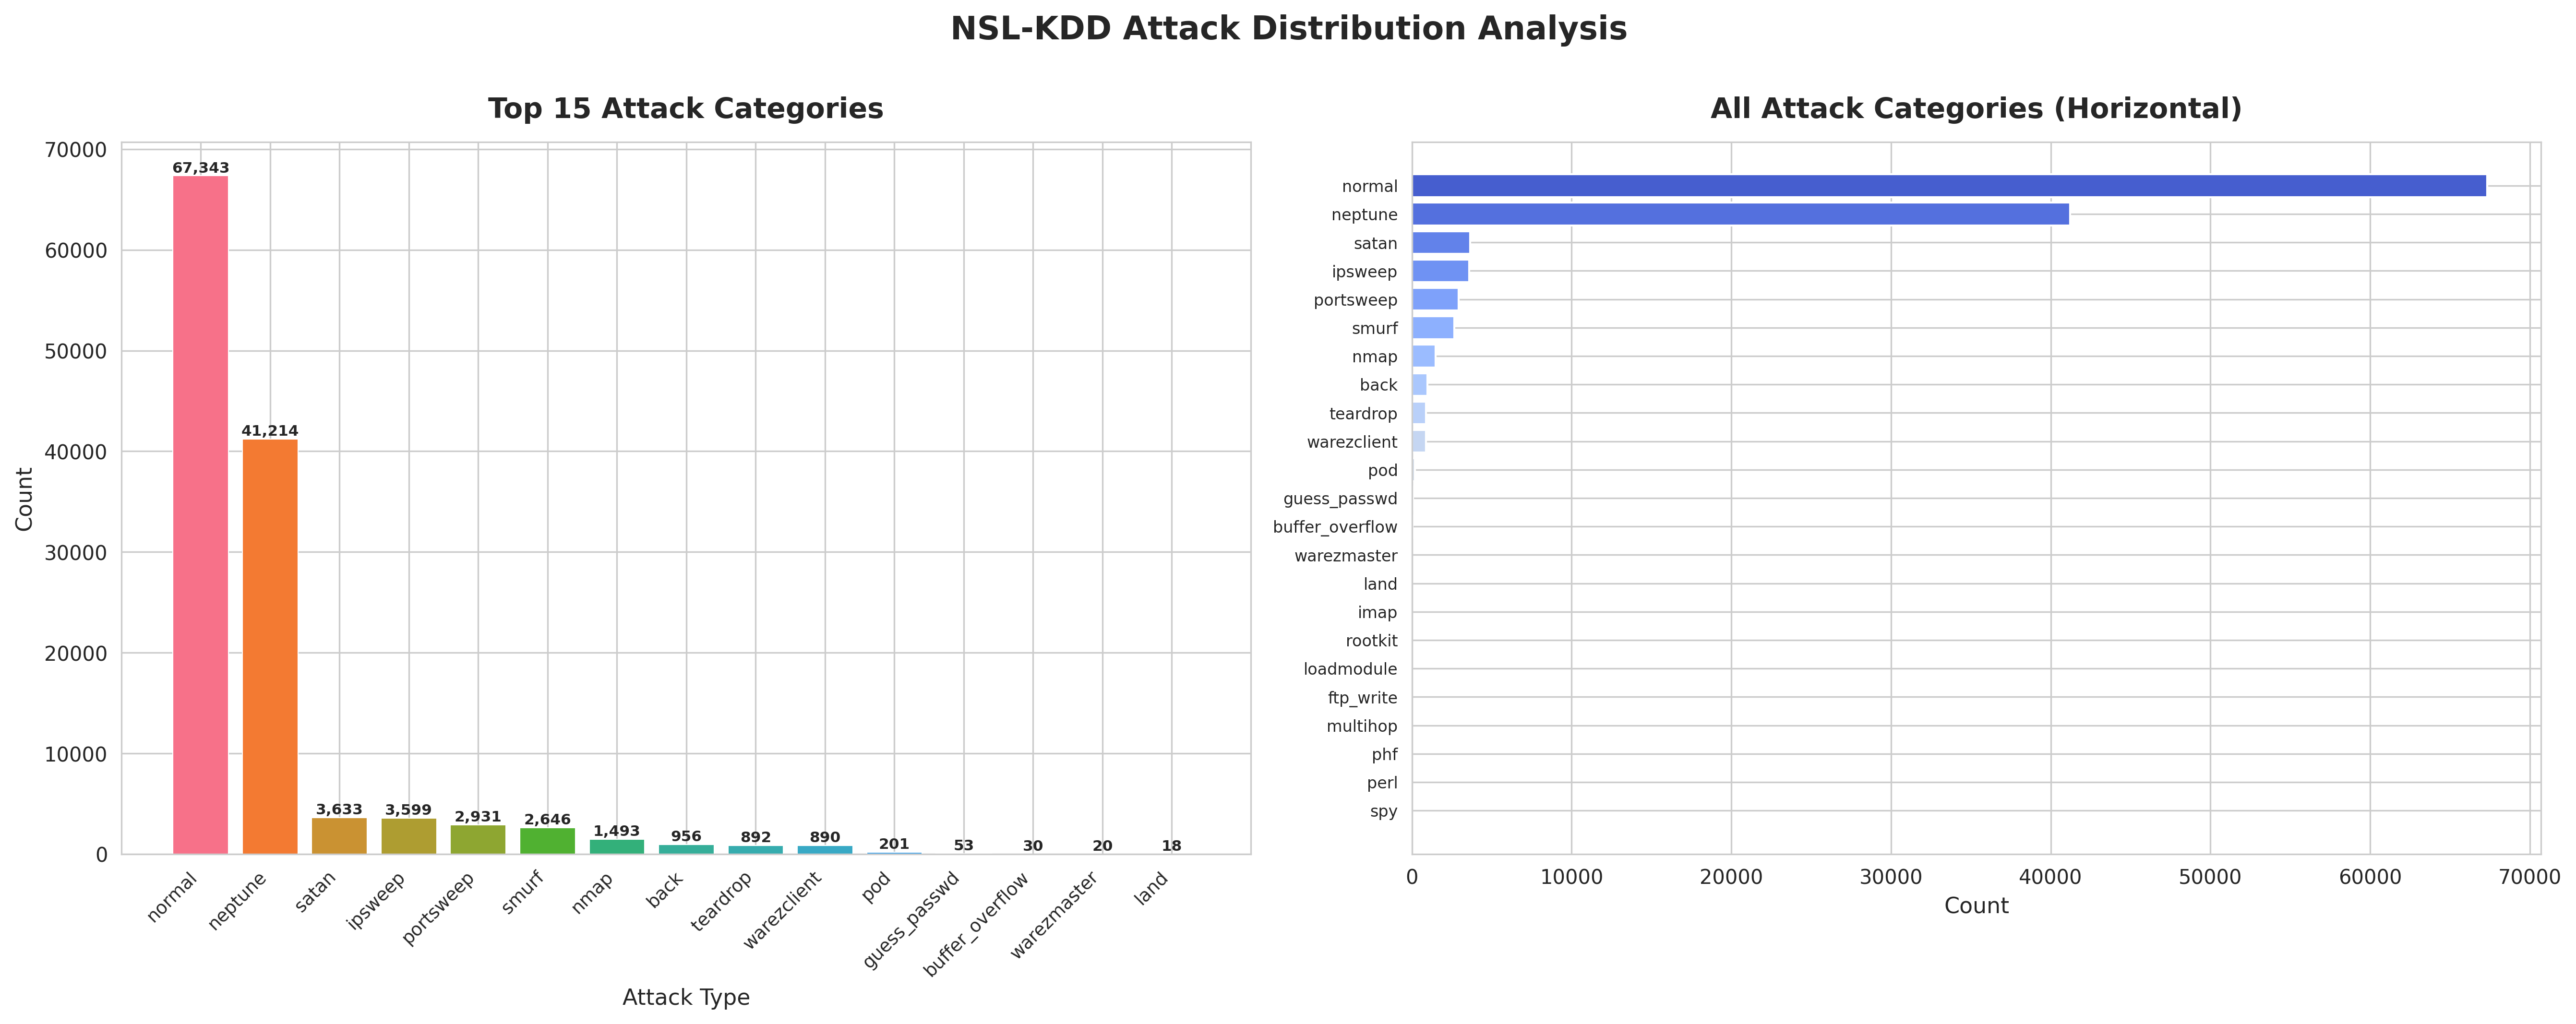
\includegraphics[width=0.85\textwidth]{figures/attack_distribution.png}
\caption{Attack Category Distribution in NSL-KDD Training Dataset}
\label{fig:attack_dist}
\end{figure}

\begin{figure}[H]
\centering
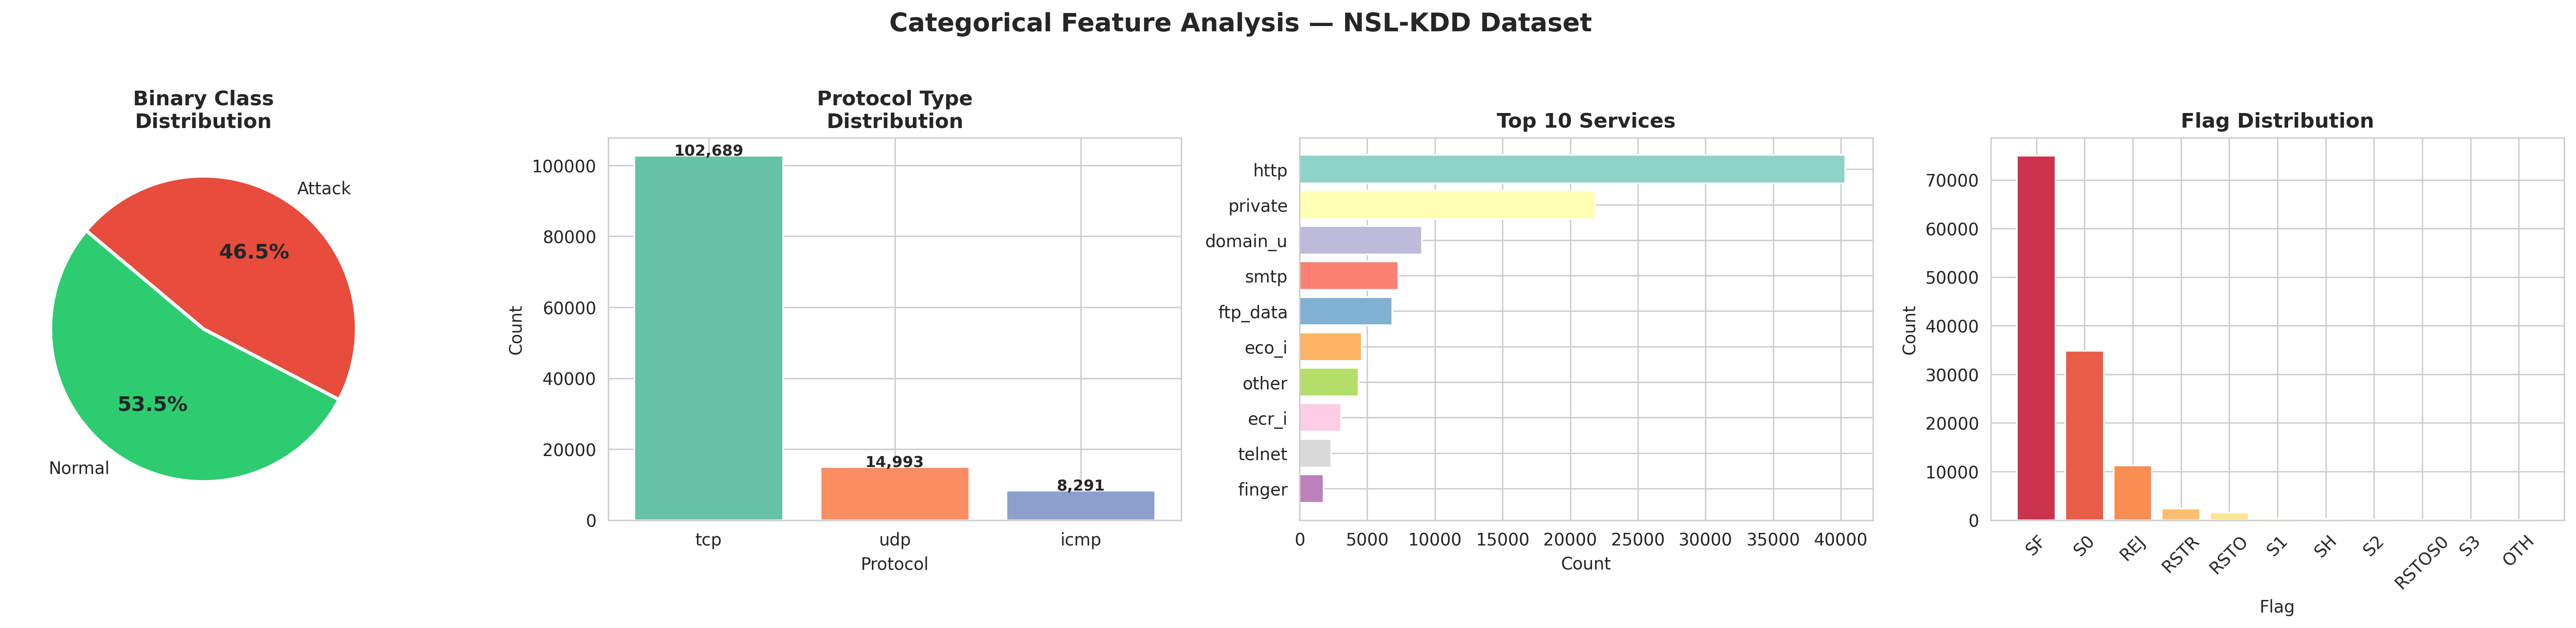
\includegraphics[width=0.9\textwidth]{figures/categorical_distributions.png}
\caption{Categorical Feature Analysis: Binary Class, Protocol Type, Services, and Connection Flags}
\label{fig:categorical}
\end{figure}

\section{Feature Explanation}

The NSL-KDD dataset contains 41 features categorized into four groups:

\textbf{Basic Features (9 features):} duration, protocol\_type, service, flag, src\_bytes, dst\_bytes, land, wrong\_fragment, urgent

\textbf{Content Features (13 features):} hot, num\_failed\_logins, logged\_in, num\_compromised, root\_shell, su\_attempted, num\_root, num\_file\_creations, num\_shells, num\_access\_files, num\_outbound\_cmds, is\_host\_login, is\_guest\_login

\textbf{Time-Based Traffic Features (9 features):} count, srv\_count, serror\_rate, srv\_serror\_rate, rerror\_rate, srv\_rerror\_rate, same\_srv\_rate, diff\_srv\_rate, srv\_diff\_host\_rate

\textbf{Host-Based Traffic Features (10 features):} dst\_host\_count, dst\_host\_srv\_count, dst\_host\_same\_srv\_rate, dst\_host\_diff\_srv\_rate, dst\_host\_same\_src\_port\_rate, dst\_host\_srv\_diff\_host\_rate, dst\_host\_serror\_rate, dst\_host\_srv\_serror\_rate, dst\_host\_rerror\_rate, dst\_host\_srv\_rerror\_rate

Categorical features include protocol\_type (tcp, udp, icmp), service (66 unique network services), and flag (11 connection status indicators).

\section{Dataset Usage}

The dataset serves dual purposes in this research: model training and performance evaluation. The training set exclusively informs model parameter learning through backpropagation, while the test set provides unbiased generalization assessment.

Preprocessing steps applied to the dataset include:
\begin{enumerate}
    \item Removal of non-predictive columns (attack name, difficulty level)
    \item Label encoding of categorical variables (protocol\_type, service, flag)
    \item StandardScaler normalization of all features
    \item Class weight computation for imbalanced learning
    \item Reshaping to 3D tensors (samples $\times$ features $\times$ 1) for LSTM input
\end{enumerate}

\section{Data Quality Issues}

Analysis identified the following data quality characteristics:

\textbf{Missing Values:} Zero missing values detected across both training and test datasets, eliminating imputation requirements.

\textbf{Class Imbalance:} Training data exhibits 53.46\% normal versus 46.54\% attack distribution. Class weights (0.9353 for normal, 1.0743 for attack) address this imbalance during training.

\textbf{Feature Correlations:} 15 feature pairs demonstrate correlation coefficients $|r| \geq 0.80$, indicating potential multicollinearity. Highly correlated pairs include dst\_host\_srv\_count with dst\_host\_same\_srv\_rate ($r = 0.97$) and serror\_rate with dst\_host\_serror\_rate ($r = 0.94$).

\textbf{Outlier Presence:} Box plot analysis reveals substantial outliers across numerical features, particularly src\_bytes and dst\_bytes. Outliers are retained as they represent legitimate network traffic characteristics including large file transfers.

\textbf{Distribution Characteristics:} Feature distributions exhibit significant right skewness (e.g., src\_bytes skew = 9.84) requiring normalization for neural network training stability.

Figure~\ref{fig:correlation} presents the feature correlation heatmap for all numerical attributes in the NSL-KDD dataset. The visualization employs a coolwarm color scheme where red indicates positive correlation, blue indicates negative correlation, and white represents near-zero correlation. The triangular masking focuses attention on the lower matrix, eliminating redundant symmetric information. Several critical correlation patterns emerge from this analysis. The upper-left region reveals strong positive correlations exceeding 0.90 between related error rate features, particularly serror\_rate and its host-based counterpart dst\_host\_serror\_rate (correlation approximately 0.94). This high correlation indicates that SYN error rates measured at the connection level strongly predict host-level SYN error rates, suggesting that both features capture similar underlying network behavior. Similarly, the same\_srv\_rate and dst\_host\_same\_srv\_rate exhibit near-perfect correlation (approximately 0.97), reflecting that connection-level service continuity strongly indicates host-level service patterns. These high correlations necessitate careful consideration during feature selection, as redundant features provide no additional discriminative information while increasing model complexity and overfitting risk. The heatmap also reveals negative correlations between diff\_srv\_rate and same\_srv\_rate (approximately -0.85), which is mathematically expected as these represent complementary proportions. The central region of the heatmap shows moderate correlations (0.30 to 0.70) between byte transfer features and connection count features, indicating that larger data transfers tend to associate with sustained connection patterns.

Figure~\ref{fig:distributions} displays the probability density distributions for 12 key numerical features, comparing normal traffic (green) against attack traffic (red). Each subplot reveals distinct separation patterns that inform model discriminative capacity. The src\_bytes distribution demonstrates pronounced bimodality for attack traffic, with one peak at near-zero values (scanning activity) and another at high values (data exfiltration), while normal traffic concentrates at lower byte counts. This bimodal pattern explains why src\_bytes emerges as the most important feature in Random Forest analysis. The dst\_bytes distribution similarly shows attack traffic extending toward higher values, reflecting denial-of-service attacks receiving large response volumes. The same\_srv\_rate subplot reveals the clearest class separation, with normal traffic concentrated near 1.0 (consistent service usage) while attack traffic spreads across the range, particularly clustering at low values indicating service scanning behavior. The count and srv\_count features both show attack traffic skewing toward higher connection counts, consistent with brute-force and scanning attack patterns. These distributional differences validate the classification approach, as the features contain sufficient discriminative signal to separate classes.

Figure~\ref{fig:boxplots} presents box plot analysis for the same 12 features, organized by class label with normal traffic (green) on the left and attack traffic (red) on the right of each subplot. The box plots reveal distributional spread through quartile boundaries, with whiskers extending to 1.5 times the interquartile range and individual points marking outliers beyond this range. The src\_bytes box plot demonstrates dramatically higher median and interquartile range for attack traffic compared to normal, with the attack box extending beyond the plot limits indicating extreme values clipped for visualization. This pattern confirms that attack traffic involves both minimal byte transfers (probes) and massive transfers (exfiltration). The hot feature (number of ``hot'' indicators suggesting suspicious activity) shows zero median for normal traffic but positive median for attack traffic, with the attack box plot revealing substantial interquartile spread indicating variable attack sophistication. The num\_compromised feature (number of compromised conditions) exhibits zero values for most normal traffic while showing positive outliers for attack traffic, directly capturing intrusion impact indicators. These box plots guide outlier treatment decisions, confirming that extreme values in features like src\_bytes represent legitimate attack characteristics rather than data recording errors.

\begin{figure}[H]
\centering
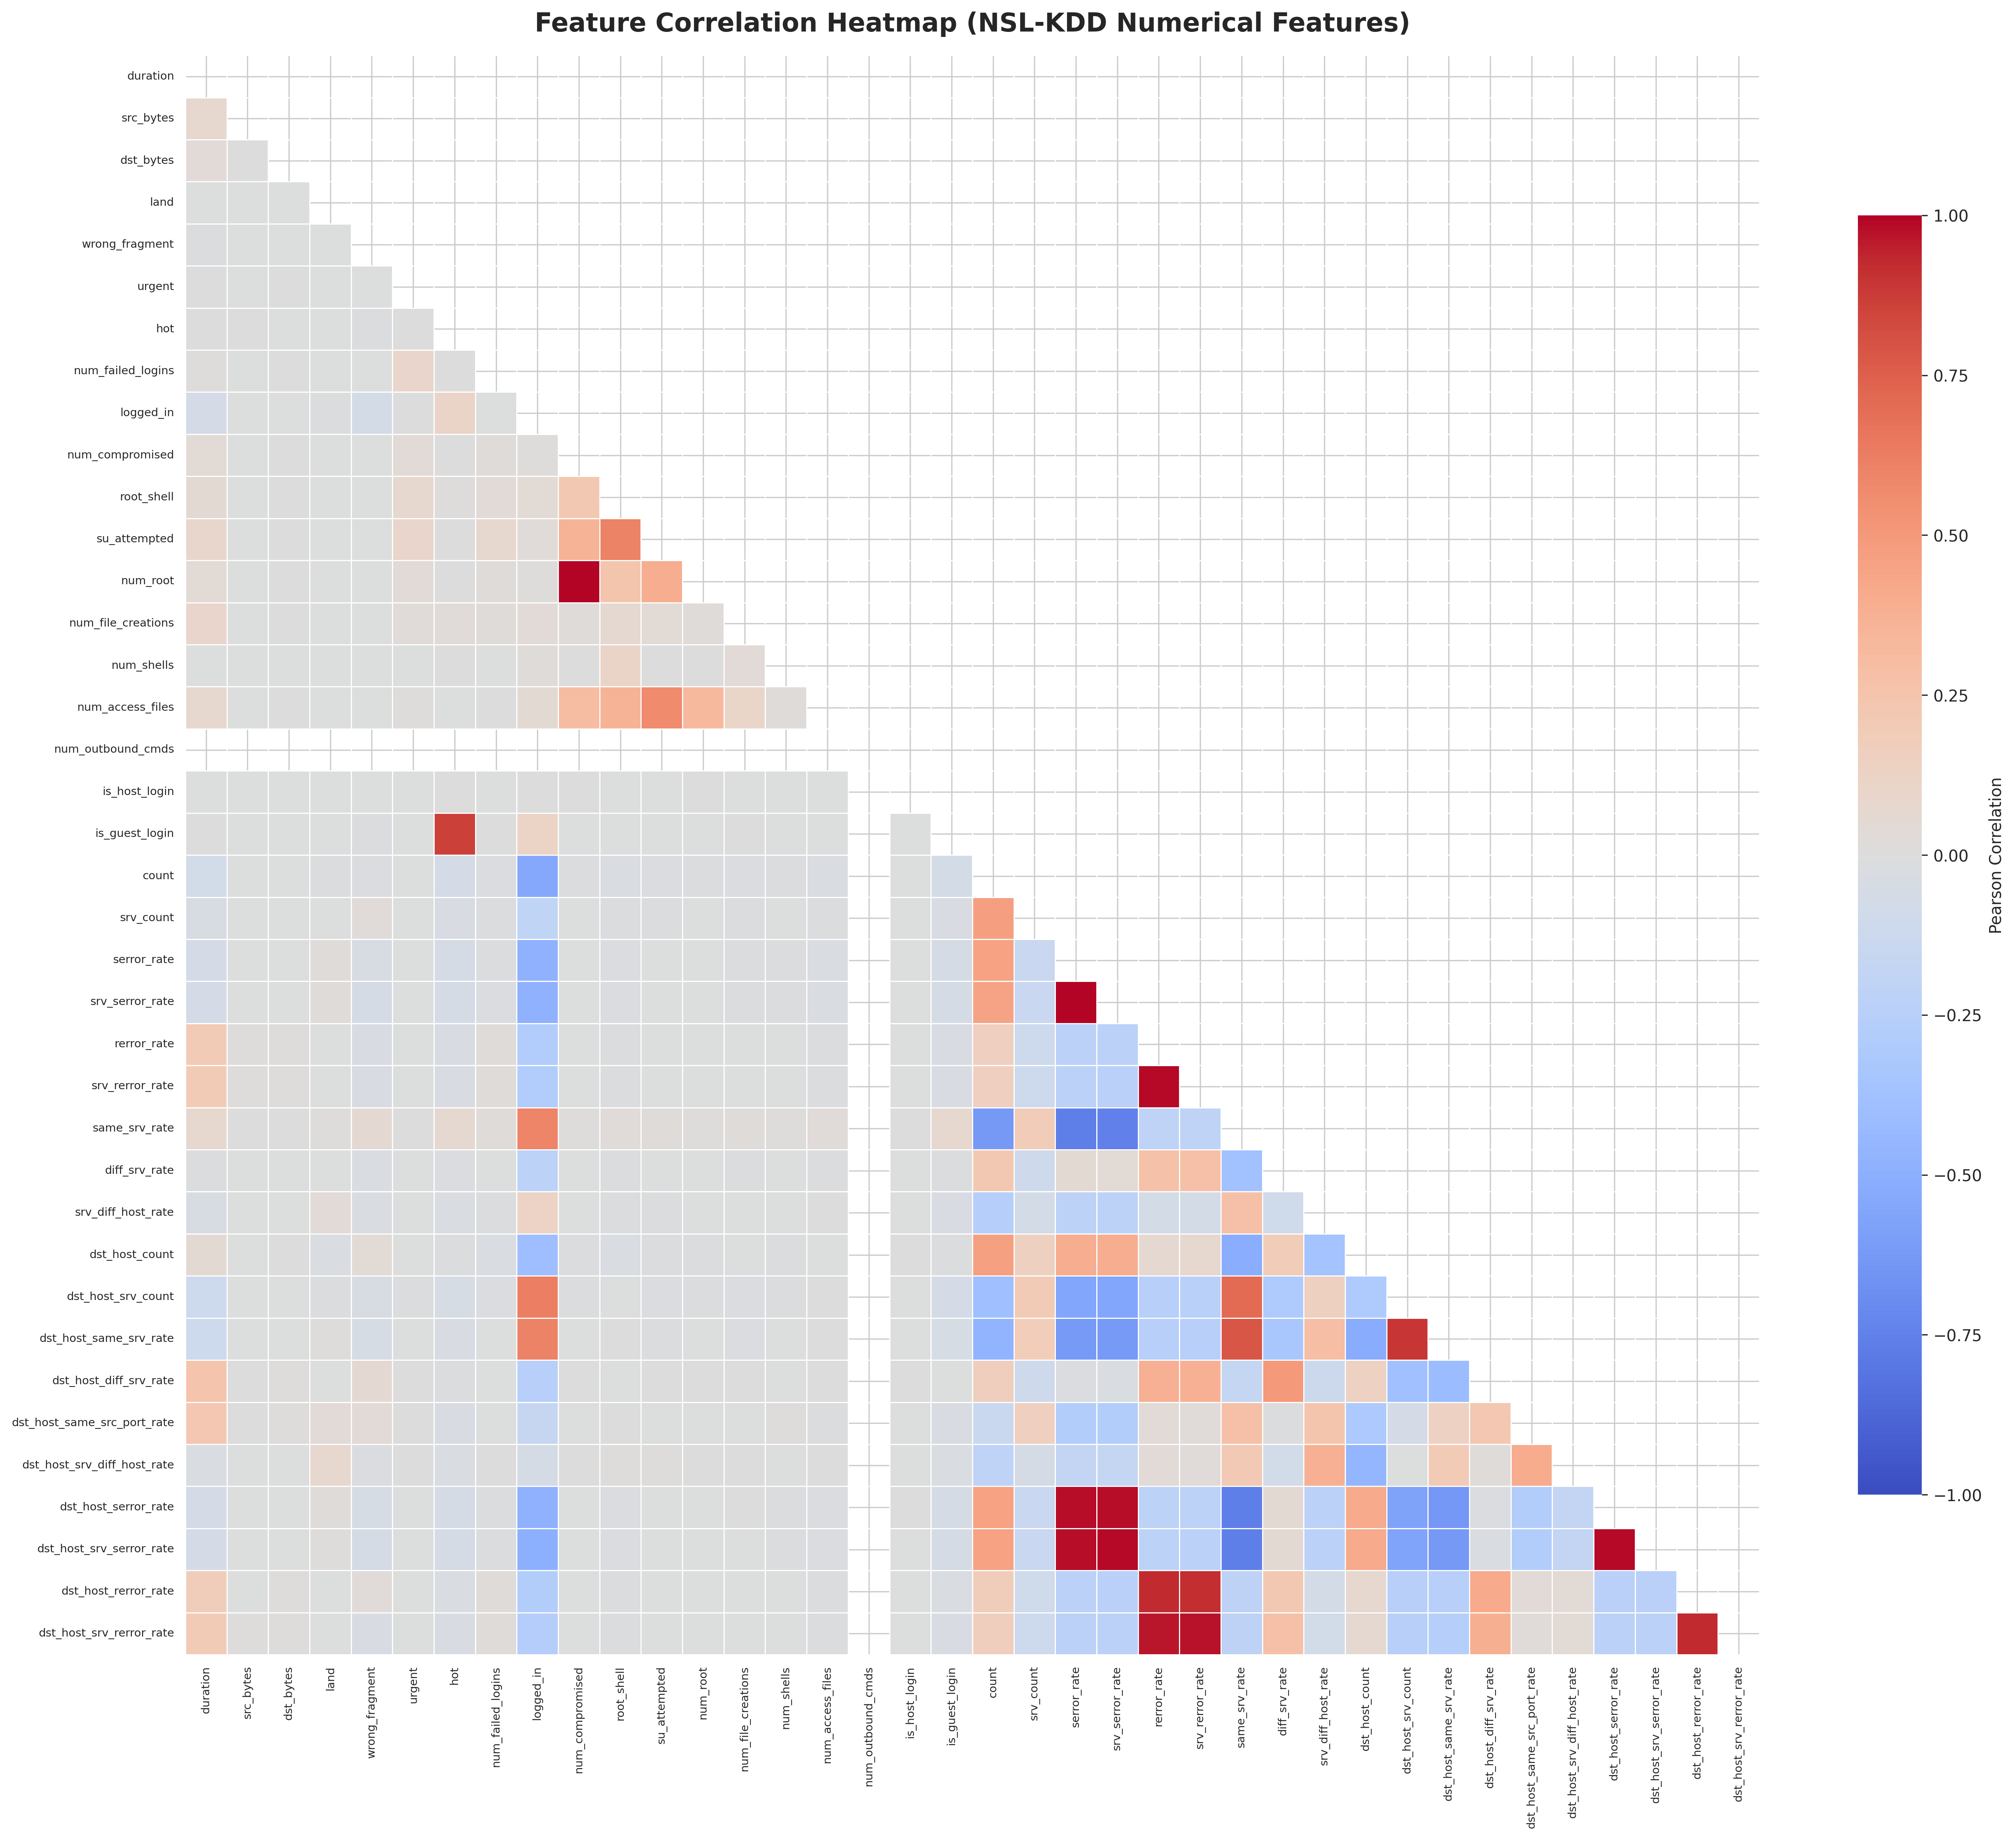
\includegraphics[width=0.9\textwidth]{figures/correlation_heatmap.png}
\caption{Feature Correlation Heatmap for NSL-KDD Numerical Features}
\label{fig:correlation}
\end{figure}

\begin{figure}[H]
\centering
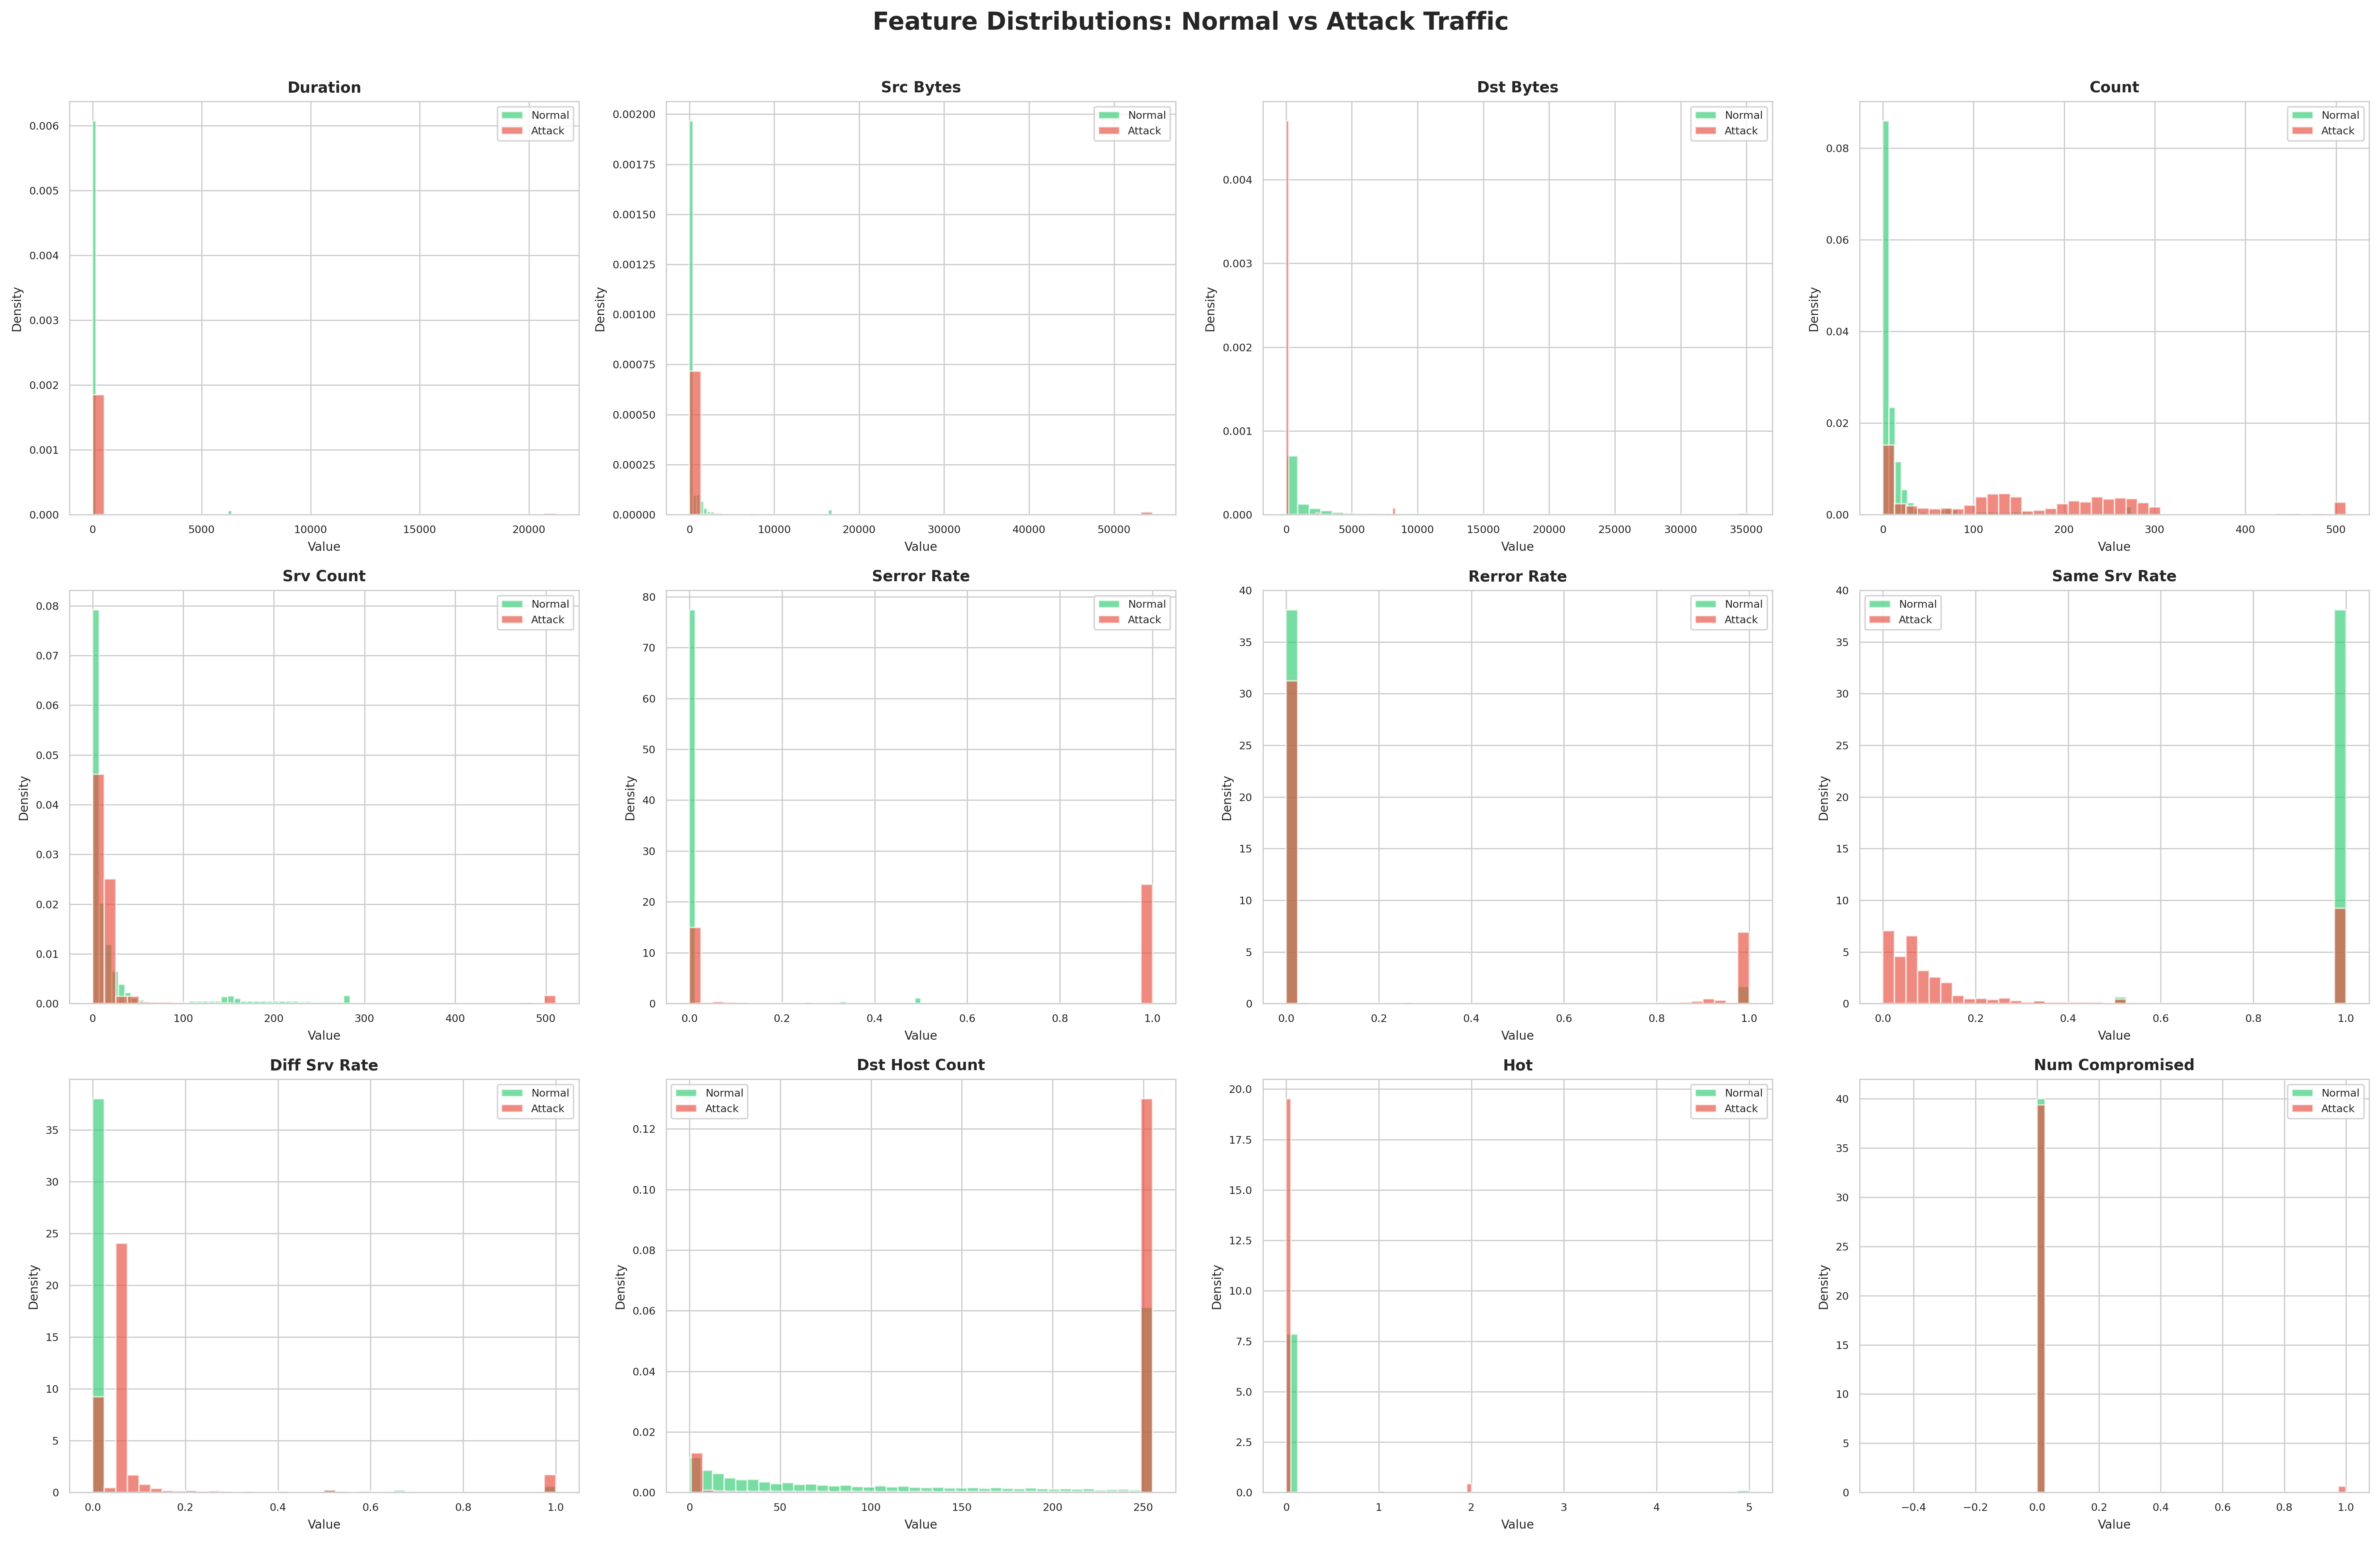
\includegraphics[width=0.95\textwidth]{figures/feature_distributions_by_class.png}
\caption{Feature Distributions by Class: Normal vs Attack Traffic Patterns}
\label{fig:distributions}
\end{figure}

\begin{figure}[H]
\centering
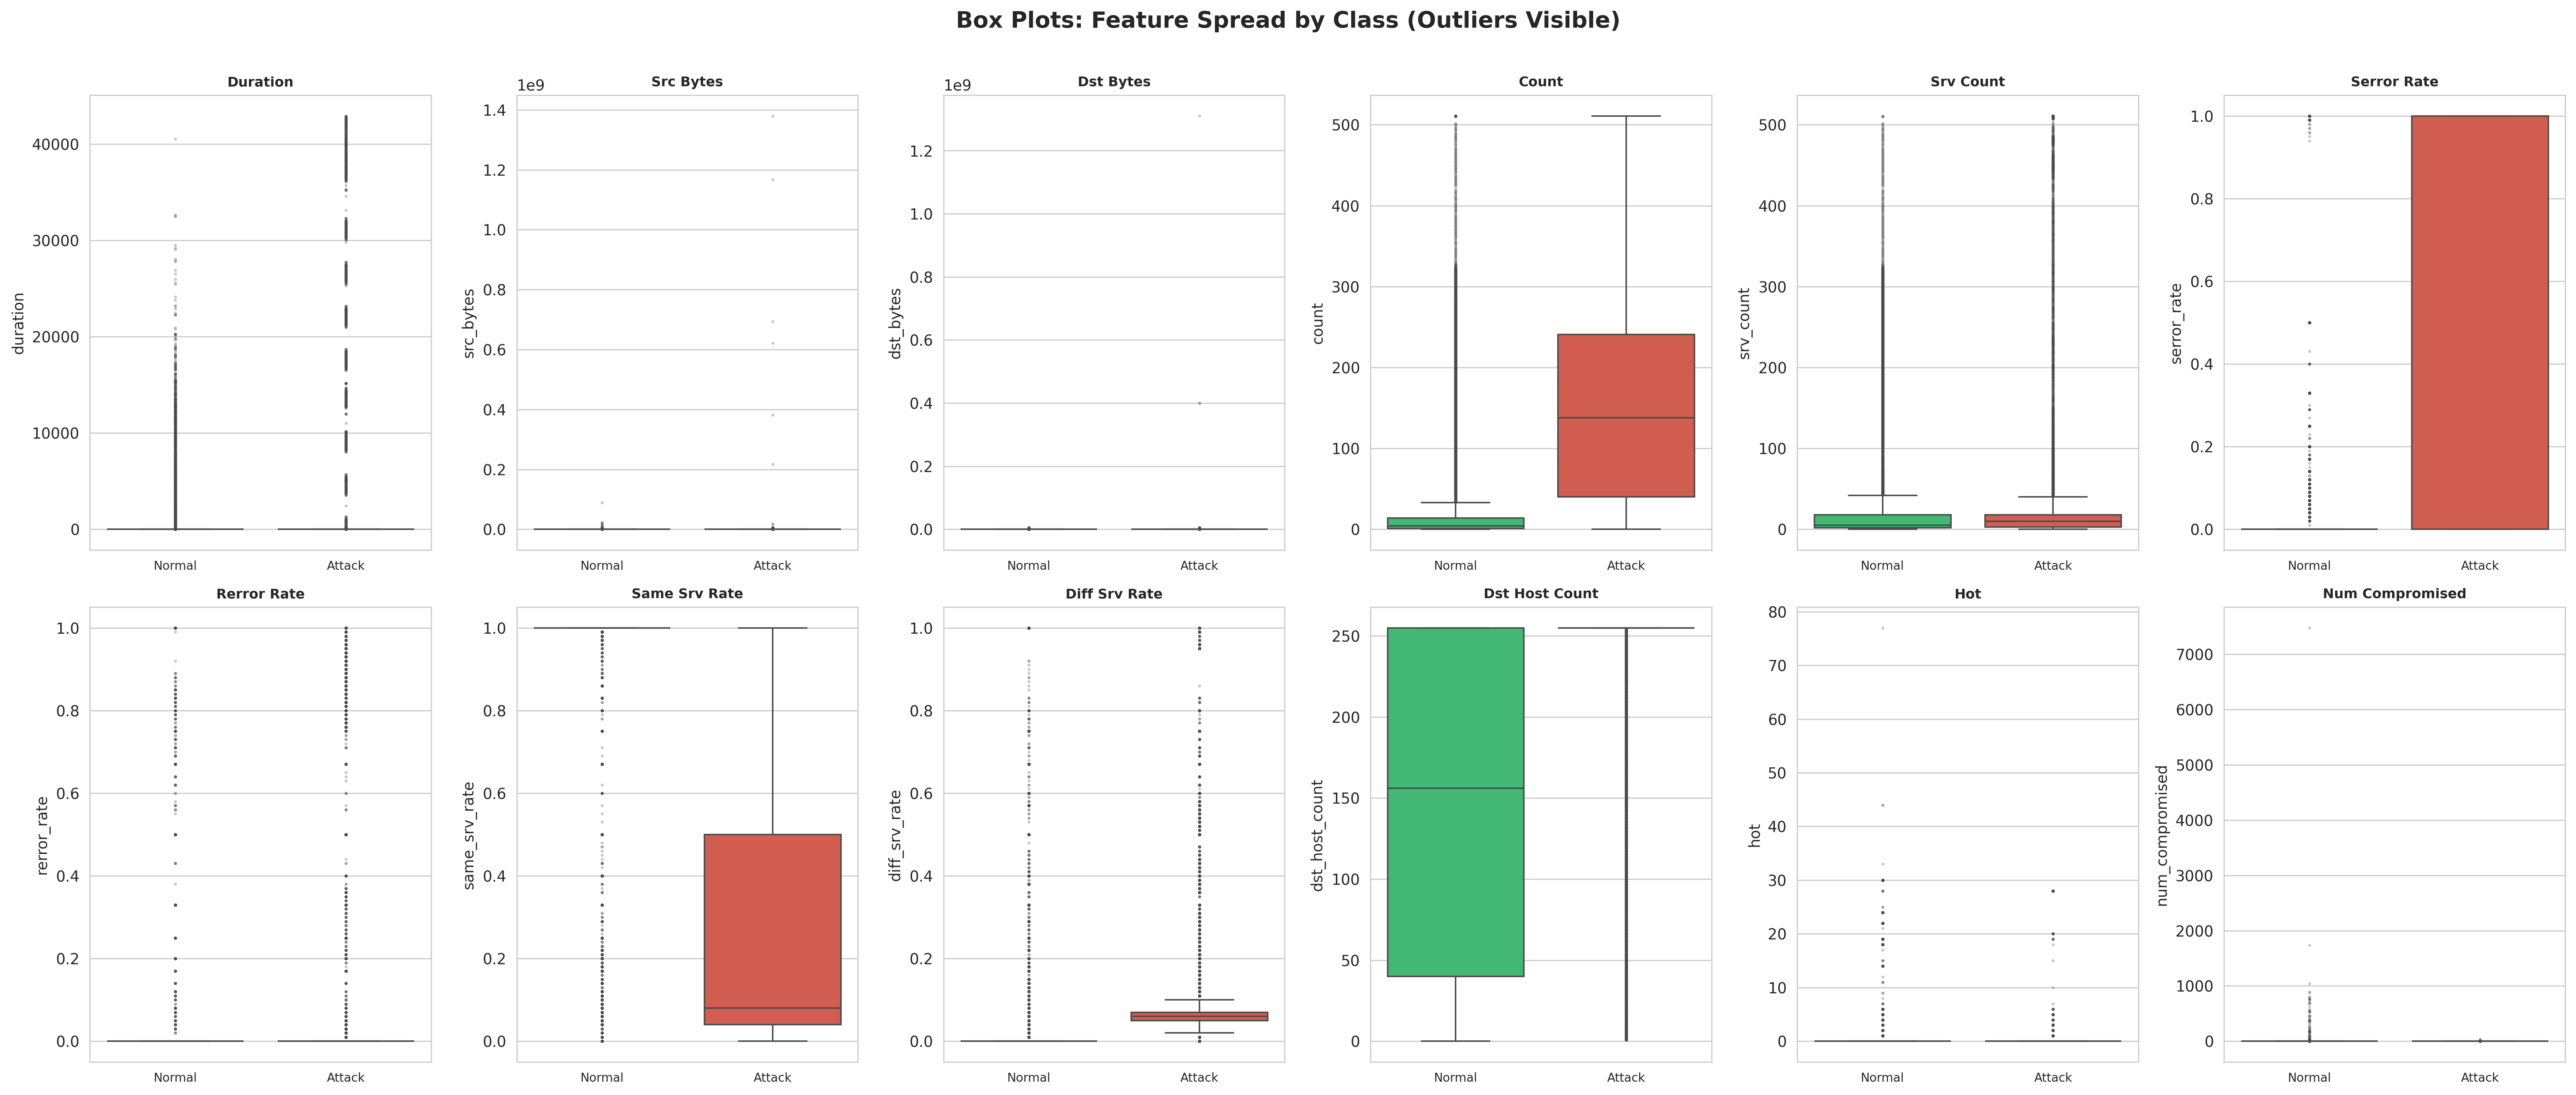
\includegraphics[width=0.95\textwidth]{figures/boxplots_by_class.png}
\caption{Box Plot Analysis: Feature Spread by Class with Outlier Detection}
\label{fig:boxplots}
\end{figure}

% ═════════════════════════════════════════════════════════════════════════════
% CHAPTER 6: METHODOLOGY
% ═════════════════════════════════════════════════════════════════════════════
\chapter{Methodology}

This chapter presents the complete methodological framework encompassing system architecture, data preprocessing, model design with mathematical formulation, algorithm workflows, tools and libraries, and experimental setup ensuring reproducibility.

\section{System Architecture}

The implemented system follows a modular pipeline architecture comprising five sequential stages: Data Ingestion, Preprocessing, Model Training, Evaluation, and Blockchain Logging. Figure~\ref{fig:architecture} illustrates the high-level system design.

\begin{figure}[H]
\centering
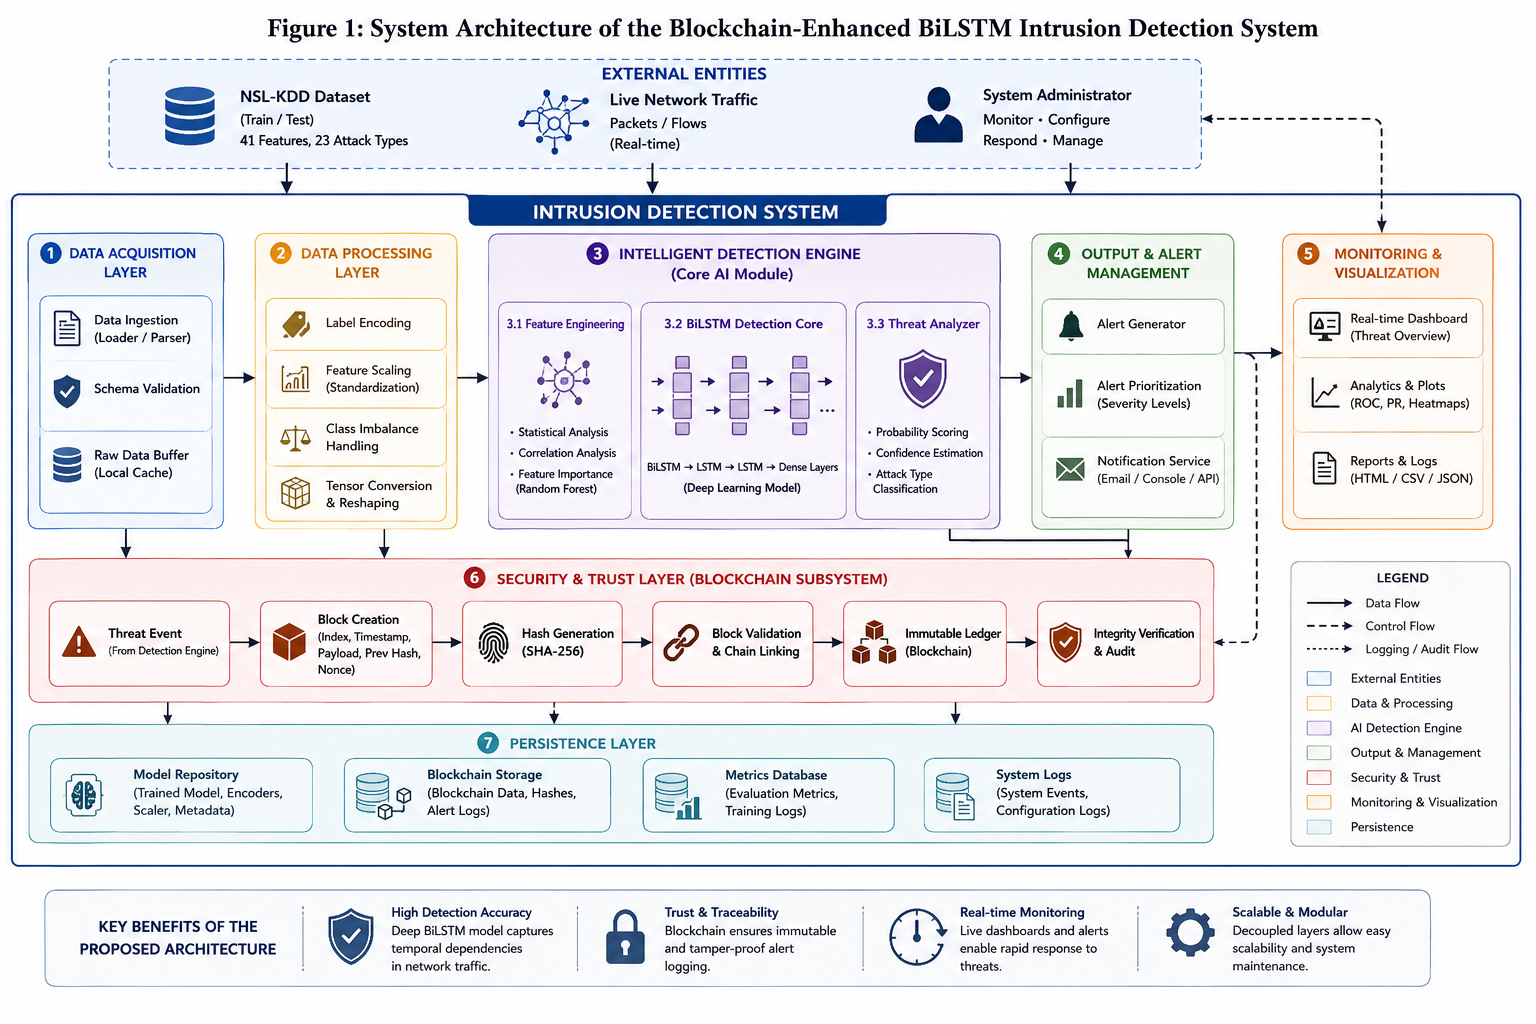
\includegraphics[width=0.9\textwidth]{figures/architecture.png}
\caption{System Architecture Overview}
\label{fig:architecture}
\end{figure}

\section{Data Preprocessing}

The preprocessing pipeline transforms raw network traffic data into LSTM-compatible tensor representations through sequential operations.

\subsection{Categorical Encoding}

Label encoding converts categorical features (protocol\_type, service, flag) to integer representations. The encoding vocabulary is fitted on combined training and test data to ensure consistent mappings:

\begin{equation}
    x_{encoded} = \text{LabelEncoder}(x_{categorical}), \quad x \in \{\text{protocol\_type}, \text{service}, \text{flag}\}
\end{equation}

Protocol\_type encodes to 3 classes, service to 66 classes, and flag to 11 classes.

\subsection{Feature Scaling}

StandardScaler normalizes features to zero mean and unit variance, preventing gradient instability during neural network training:

\begin{equation}
    z = \frac{x - \mu}{\sigma}, \quad \mu = \frac{1}{N}\sum_{i=1}^{N} x_i, \quad \sigma = \sqrt{\frac{1}{N}\sum_{i=1}^{N}(x_i - \mu)^2}
\end{equation}

The scaler is fitted exclusively on training data to prevent data leakage, with fitted parameters applied to test data transformation.

\subsection{Class Weight Computation}

Balanced class weights address training bias toward the majority class:

\begin{equation}
    w_j = \frac{N}{k \cdot n_j}, \quad j \in \{0, 1\}
\end{equation}

where $N = 125,973$ is total samples, $k = 2$ is number of classes, and $n_j$ is samples per class. Computed weights are 0.9353 for normal (class 0) and 1.0743 for attack (class 1).

\subsection{LSTM Reshaping}

The 2D feature matrix reshapes to 3D tensors adding a singleton dimension for LSTM channel processing:

\begin{equation}
    X \in \mathbb{R}^{N \times 41} \rightarrow X_{LSTM} \in \mathbb{R}^{N \times 41 \times 1}
\end{equation}

Final training tensor dimensions: $(125973 \times 41 \times 1)$.

\section{Model Design and Mathematical Formulation}

The implemented architecture is a stacked bidirectional LSTM neural network with dense classification head.

\subsection{Bidirectional LSTM Layer}

The LSTM cell operates through gating mechanisms controlling information flow:

\begin{align}
    f_t &= \sigma(W_f \cdot [h_{t-1}, x_t] + b_f) \quad \text{(forget gate)} \\
    i_t &= \sigma(W_i \cdot [h_{t-1}, x_t] + b_i) \quad \text{(input gate)} \\
    \tilde{C}_t &= \tanh(W_C \cdot [h_{t-1}, x_t] + b_C) \quad \text{(candidate state)} \\
    C_t &= f_t \odot C_{t-1} + i_t \odot \tilde{C}_t \quad \text{(cell state)} \\
    o_t &= \sigma(W_o \cdot [h_{t-1}, x_t] + b_o) \quad \text{(output gate)} \\
    h_t &= o_t \odot \tanh(C_t) \quad \text{(hidden state)}
\end{align}

where $\sigma$ denotes sigmoid activation, $\odot$ element-wise multiplication, and $W$, $b$ learnable parameters.

Bidirectional processing concatenates forward and backward LSTM outputs:

\begin{equation}
    h_t^{bidir} = [\overrightarrow{h_t}; \overleftarrow{h_t}] \in \mathbb{R}^{2 \times units}
\end{equation}

\subsection{Architecture Specification}

Table~\ref{tab:architecture} details the implemented neural architecture.

\begin{table}[H]
\centering
\caption{Bidirectional LSTM Model Architecture}
\label{tab:architecture}
\begin{tabular}{>{\raggedright\arraybackslash}p{2.8cm}p{3.5cm}cc}
\toprule
\textbf{Layer} & \textbf{Configuration} & \textbf{Output Shape} & \textbf{Params} \\
\midrule
Input & Features $\times$ Channels & (41, 1) & 0 \\
Bidirectional LSTM & 128 units, L2=1e-4 & (41, 256) & 133,120 \\
Batch Normalization & Axis=-1 & (41, 256) & 1,024 \\
Dropout & Rate=0.35 & (41, 256) & 0 \\
LSTM & 96 units, L2=1e-4 & (41, 96) & 135,168 \\
Batch Normalization & Axis=-1 & (41, 96) & 384 \\
Dropout & Rate=0.30 & (41, 96) & 0 \\
LSTM & 64 units, L2=1e-4 & (64,) & 41,216 \\
Batch Normalization & Axis=-1 & (64,) & 256 \\
Dropout & Rate=0.25 & (64,) & 0 \\
Dense & 128 units, ReLU, L2=1e-4 & (128,) & 8,320 \\
Batch Normalization & Axis=-1 & (128,) & 512 \\
Dropout & Rate=0.20 & (128,) & 0 \\
Dense & 64 units, ReLU, L2=1e-4 & (64,) & 8,256 \\
Dropout & Rate=0.15 & (64,) & 0 \\
Output & 1 unit, Sigmoid & (1,) & 65 \\
\midrule
\multicolumn{2}{l}{\textbf{Total Parameters}} & & \textbf{328,705} \\
\bottomrule
\end{tabular}
\end{table}

\subsection{Loss Function}

Binary cross-entropy loss with class weighting:

\begin{equation}
    \mathcal{L} = -\frac{1}{N} \sum_{i=1}^{N} w_{y_i} \left[ y_i \log(\hat{y}_i) + (1-y_i) \log(1-\hat{y}_i) \right]
\end{equation}

where $\hat{y}_i = \sigma(z_i)$ is the predicted probability and $w_{y_i}$ is the class weight.

\subsection{Optimization}

Adam optimizer with gradient clipping:

\begin{align}
    m_t &= \beta_1 m_{t-1} + (1-\beta_1) g_t \\
    v_t &= \beta_2 v_{t-1} + (1-\beta_2) g_t^2 \\
    \hat{m}_t &= \frac{m_t}{1-\beta_1^t}, \quad \hat{v}_t = \frac{v_t}{1-\beta_2^t} \\
    \theta_{t+1} &= \theta_t - \frac{\eta}{\sqrt{\hat{v}_t} + \epsilon} \hat{m}_t
\end{align}

Configuration: learning rate $\eta = 0.001$, $\beta_1 = 0.9$, $\beta_2 = 0.999$, gradient clipnorm = 1.0.

\section{Algorithm Workflow and Pseudocode}

Algorithm~\ref{alg:training} presents the complete training workflow.

\begin{algorithm}[H]
\caption{Bidirectional LSTM Training Workflow}
\label{alg:training}
\begin{algorithmic}[1]
\Require Training data $X_{train}$, labels $y_{train}$, validation split $v=0.2$
\Ensure Trained model parameters $\theta^*$
\State Initialize model architecture with 328,705 parameters
\State Compute class weights: $w_0 = 0.9353$, $w_1 = 1.0743$
\State Configure Adam optimizer: $\eta = 0.001$, clipnorm = 1.0
\State Reshape input: $X_{LSTM} \in \mathbb{R}^{N \times 41 \times 1}$
\State Initialize callbacks: EarlyStopping, ReduceLROnPlateau, ModelCheckpoint, CSVLogger
\State $best\_auc \leftarrow 0$, $patience \leftarrow 7$
\For{$epoch = 1$ to $50$}
    \For{each batch $b$ in $X_{LSTM}$}
        \State Forward pass: compute predictions $\hat{y} = f(X_b; \theta)$
        \State Compute weighted loss: $\mathcal{L}_b = \text{BinaryCrossEntropy}(y_b, \hat{y}, w)$
        \State Backward pass: compute gradients $\nabla_\theta \mathcal{L}_b$
        \State Clip gradients: $g \leftarrow \text{clip}(g, -1.0, 1.0)$
        \State Update parameters: $\theta \leftarrow \theta - \eta \cdot \text{Adam}(\nabla_\theta \mathcal{L})$
    \EndFor
    \State Evaluate on validation set: $val\_auc \leftarrow \text{AUC}(y_{val}, \hat{y}_{val})$
    \State Log metrics: accuracy, loss, precision, recall, AUC
    \If{$val\_auc > best\_auc$}
        \State $best\_auc \leftarrow val\_auc$
        \State Save model checkpoint
    \EndIf
    \If{no improvement for 7 epochs}
        \State Restore best weights and terminate
    \EndIf
    \If{no improvement for 3 epochs}
        \State $\eta \leftarrow \eta \times 0.5$
    \EndIf
\EndFor
\State \Return $\theta^*$
\end{algorithmic}
\end{algorithm}

\section{Tools and Libraries}

Table~\ref{tab:tools} enumerates the software stack and library versions.

\begin{table}[H]
\centering
\caption{Implementation Tools and Libraries}
\label{tab:tools}
\begin{tabular}{lll}
\toprule
\textbf{Category} & \textbf{Library/Tool} & \textbf{Version/Purpose} \\
\midrule
Deep Learning & TensorFlow & 2.x, GPU-accelerated training \\
Deep Learning & Keras & Model API and callbacks \\
Data Processing & NumPy & Numerical computations \\
Data Processing & Pandas & Data frame operations \\
Machine Learning & Scikit-learn & Metrics, preprocessing, PCA, t-SNE \\
Visualization & Matplotlib & Static figure generation \\
Visualization & Seaborn & Statistical visualization \\
Persistence & Joblib & Model serialization \\
Utilities & TQDM & Progress bars \\
Blockchain & Hashlib (Python stdlib) & SHA-256 hashing \\
Environment & Kaggle & GPU runtime (2x T4) \\
\bottomrule
\end{tabular}
\end{table}

\section{Experimental Setup and Reproducibility}

\subsection{Hardware Configuration}

Training executed on Kaggle cloud infrastructure with:
\begin{itemize}
    \item GPU: 2x NVIDIA T4 Tensor Core GPUs
    \item GPU Memory: 16GB per device (32GB total)
    \item System Memory: 32GB RAM
    \item Storage: 20GB persistent storage
\end{itemize}

\subsection{Software Configuration}

\begin{itemize}
    \item Python: 3.10+
    \item TensorFlow: 2.x (GPU-enabled)
    \item CUDA: 11.x
    \item cuDNN: 8.x
    \item Mixed Precision: Enabled (float16)
\end{itemize}

\subsection{Hyperparameters}

Fixed hyperparameters ensuring reproducibility:
\begin{itemize}
    \item Random Seed: 42
    \item Epochs: 50 (early stopping at epoch 19)
    \item Batch Size: 256
    \item Validation Split: 0.20
    \item L2 Regularization: 1e-4
    \item Dropout Rates: [0.35, 0.30, 0.25, 0.20, 0.15]
\end{itemize}

\subsection{Reproducibility Checklist}

Complete reproduction requires:
\begin{enumerate}
    \item Dataset: KDDTrain+.txt and KDDTest+.txt from NSL-KDD
    \item Random seed initialization: np.random.seed(42), tf.random.set\_seed(42)
    \item GPU memory growth enabling before model construction
    \item Exact preprocessing order: encode $\rightarrow$ scale $\rightarrow$ reshape
    \item Callback configuration matching specified parameters
\end{enumerate}

Run ID 20260510\_164507 identifies the specific execution documented in this report. All artifacts (model weights, logs, visualizations) reference this identifier.

% ═════════════════════════════════════════════════════════════════════════════
% CHAPTER 7: OUTCOMES AND RESULTS
% ═════════════════════════════════════════════════════════════════════════════
\chapter{Outcomes and Results}

This chapter presents the complete experimental outcomes including evaluation metrics, quantitative results, qualitative analysis, discussion of findings, and practical application considerations.

\section{Evaluation Metrics}

The framework reports eight primary metrics providing comprehensive performance characterization:

\textbf{Accuracy:} Overall correct classification rate:
\begin{equation}
    Accuracy = \frac{TP + TN}{TP + TN + FP + FN} = \frac{8442 + 9521}{22544} = 0.7968
\end{equation}

\textbf{Precision:} Attack detection reliability:
\begin{equation}
    Precision = \frac{TP}{TP + FP} = \frac{8442}{8442 + 190} = 0.9780
\end{equation}

\textbf{Recall (TPR):} Attack detection completeness:
\begin{equation}
    Recall = \frac{TP}{TP + FN} = \frac{8442}{8442 + 4391} = 0.6578
\end{equation}

\textbf{Specificity (TNR):} Normal traffic preservation:
\begin{equation}
    Specificity = \frac{TN}{TN + FP} = \frac{9521}{9521 + 190} = 0.9804
\end{equation}

\textbf{F1-Score:} Precision-recall harmonic mean:
\begin{equation}
    F1 = 2 \cdot \frac{Precision \cdot Recall}{Precision + Recall} = 0.7866
\end{equation}

\textbf{Matthews Correlation Coefficient:} Balanced measure for imbalanced data:
\begin{equation}
    MCC = \frac{TP \cdot TN - FP \cdot FN}{\sqrt{(TP+FP)(TP+FN)(TN+FP)(TN+FN)}} = 0.6502
\end{equation}

\textbf{Cohen's Kappa:} Inter-rater agreement measure:
\begin{equation}
    \kappa = \frac{p_o - p_e}{1 - p_e} = 0.6064
\end{equation}

\textbf{AUC-ROC:} Area under receiver operating characteristic curve: 0.9487

\textbf{AUC-PR:} Area under precision-recall curve: 0.9616

\section{Quantitative Results}

Table~\ref{tab:results} presents the complete test set performance metrics.

\begin{table}[H]
\centering
\caption{Comprehensive Test Set Evaluation Results}
\label{tab:results}
\begin{tabular}{lcc}
\toprule
\textbf{Metric} & \textbf{Value} & \textbf{Interpretation} \\
\midrule
Accuracy & 0.7968 & 79.68\% correct classification \\
Precision & 0.9780 & 97.8\% of alerts are true attacks \\
Recall (TPR) & 0.6578 & 65.78\% of attacks detected \\
Specificity (TNR) & 0.9804 & 98.04\% of normal traffic preserved \\
F1 Score & 0.7866 & Strong precision-recall balance \\
MCC & 0.6502 & Moderate correlation strength \\
Cohen's Kappa & 0.6064 & Substantial agreement \\
AUC-ROC & 0.9487 & Excellent discrimination \\
AUC-PR & 0.9616 & Strong precision-recall trade-off \\
False Positive Rate & 0.0196 & 1.96\% normal traffic blocked \\
Negative Predictive Value & 0.6844 & 68.44\% negative predictions correct \\
\midrule
True Positives & 8,442 & Correctly detected attacks \\
True Negatives & 9,521 & Correctly classified normal \\
False Positives & 190 & Normal misclassified as attack \\
False Negatives & 4,391 & Attacks missed (critical) \\
\bottomrule
\end{tabular}
\end{table}

Figure~\ref{fig:confusion} presents the confusion matrix analysis through two complementary visualizations: raw counts and normalized proportions. The raw counts matrix reveals the absolute classification outcomes: 9,521 true negatives (normal traffic correctly classified), 8,442 true positives (attacks correctly detected), 190 false positives (normal traffic misclassified as attack), and 4,391 false negatives (attacks missed). These counts translate to the performance metrics reported in Table~\ref{tab:results}, with the high false negative count (4,391) representing the primary system limitation. The normalized confusion matrix expresses these counts as proportions of true class membership, revealing that 98.04\% of normal traffic is correctly classified (specificity) while only 65.78\% of attacks are detected (recall). This asymmetric performance reflects the precision-recall trade-off inherent in imbalanced classification with a 0.5 decision threshold. The normalized matrix's diagonal values (0.980 for normal, 0.658 for attack) immediately communicate the classifier's conservative bias toward predicting normal traffic. This bias is quantitatively explained by the class imbalance in training data (53.46\% normal) combined with class weights that do not fully compensate for the prior distribution.

Figure~\ref{fig:roc} displays the Receiver Operating Characteristic curve plotting true positive rate against false positive rate across all classification thresholds. The blue curve representing the LSTM model demonstrates superior discriminative capacity, achieving AUC-ROC of 0.9487. The shaded area under the curve (light blue fill) represents the probability that the classifier ranks a randomly chosen attack instance higher than a randomly chosen normal instance. The curve's steep initial ascent indicates that at low false positive rates (below 0.05), the model achieves high true positive rates (above 0.60), a critical property for deployment scenarios where false alarms must be minimized. The operating point at threshold 0.5 (marked with red circle) achieves 0.6578 true positive rate at 0.0196 false positive rate, positioned near the ``elbow'' of the curve representing an optimal cost-sensitive operating point. The diagonal dashed line represents random classifier performance (AUC = 0.50), while the green dotted line represents perfect classification (AUC = 1.0). The LSTM curve's substantial separation from the random baseline confirms genuine learning rather than chance correlation.

Figure~\ref{fig:prcurve} presents the precision-recall analysis through dual subplots. The left subplot displays the precision-recall curve, which is particularly informative for imbalanced datasets where ROC curves can appear deceptively optimistic. The orange curve achieves AUC-PR of 0.9616, indicating strong precision-recall trade-offs. The baseline horizontal line at 0.569 represents the attack prevalence in the test set; curves above this baseline indicate classifier performance exceeding random guessing. The substantial area between the LSTM curve and baseline (shaded orange) quantifies the model's discriminative value added beyond trivial classifiers. The curve's shape reveals high precision (above 0.95) is achievable at moderate recall levels (0.40 to 0.60), suggesting threshold tuning could optimize for specific operational requirements. The right subplot analyzes precision and recall as functions of classification threshold, providing actionable guidance for threshold selection. At the default 0.5 threshold (vertical dotted line), precision reaches 0.978 while recall achieves 0.658. The precision curve remains relatively flat across thresholds 0.3 to 0.7, indicating robustness to threshold selection within this range. The recall curve declines steeply above threshold 0.8, suggesting that high-confidence predictions sacrifice attack detection completeness.

Figure~\ref{fig:metrics} provides a comprehensive evaluation dashboard combining metric summaries and detailed classification statistics. The left subplot presents eight key performance metrics as vertical bar charts with color-coded values: green (score $\geq$ 0.90), yellow (0.75 $\leq$ score $<$ 0.90), and red (score $<$ 0.75). This visualization immediately identifies model strengths and weaknesses: AUC-ROC (0.9487), AUC-PR (0.9616), and Specificity (0.9804) appear in green indicating excellent performance; Accuracy (0.7968), Precision (0.9780), F1-Score (0.7866), and normalized MCC (0.8251) appear in yellow indicating acceptable but improvable performance; while Recall (0.6578) stands alone in red highlighting the primary improvement target. The right subplot presents a tabular summary of confusion matrix details, providing concrete counts for forensic interpretation: 8,442 attacks correctly detected versus 4,391 missed, 9,521 normal connections preserved versus 190 incorrectly flagged. These absolute counts translate to operational impact: the system would generate approximately 190 false alarms and miss 4,391 genuine attacks when processing 22,544 connections.

Figure~\ref{fig:probability} examines model calibration through prediction probability distributions. The left subplot compares probability densities for true normal traffic (green) versus true attack traffic (red). Ideally, these distributions would exhibit minimal overlap with normal traffic concentrating near 0.0 and attack traffic near 1.0. The visualization reveals reasonable but imperfect separation: normal traffic shows strong density concentration below 0.2, while attack traffic exhibits bimodal distribution with peaks near 0.4 and 0.8. The substantial overlap region (0.3 to 0.7) contains ambiguous predictions where the model lacks confidence, contributing to classification errors. The vertical dashed line at 0.5 marks the decision threshold; the area under the red curve to the left of this line represents false negatives (attacks predicted as normal), while the area under the green curve to the right represents false positives (normal predicted as attack). The right subplot displays the overall histogram of predicted probabilities across all test instances, revealing that the model tends toward extreme predictions (peaks near 0.0 and 1.0) with fewer instances in the uncertain middle range. This U-shaped distribution indicates well-calibrated confidence: the model is decisive when features strongly indicate class membership and appropriately uncertain for ambiguous cases.

\begin{figure}[H]
\centering
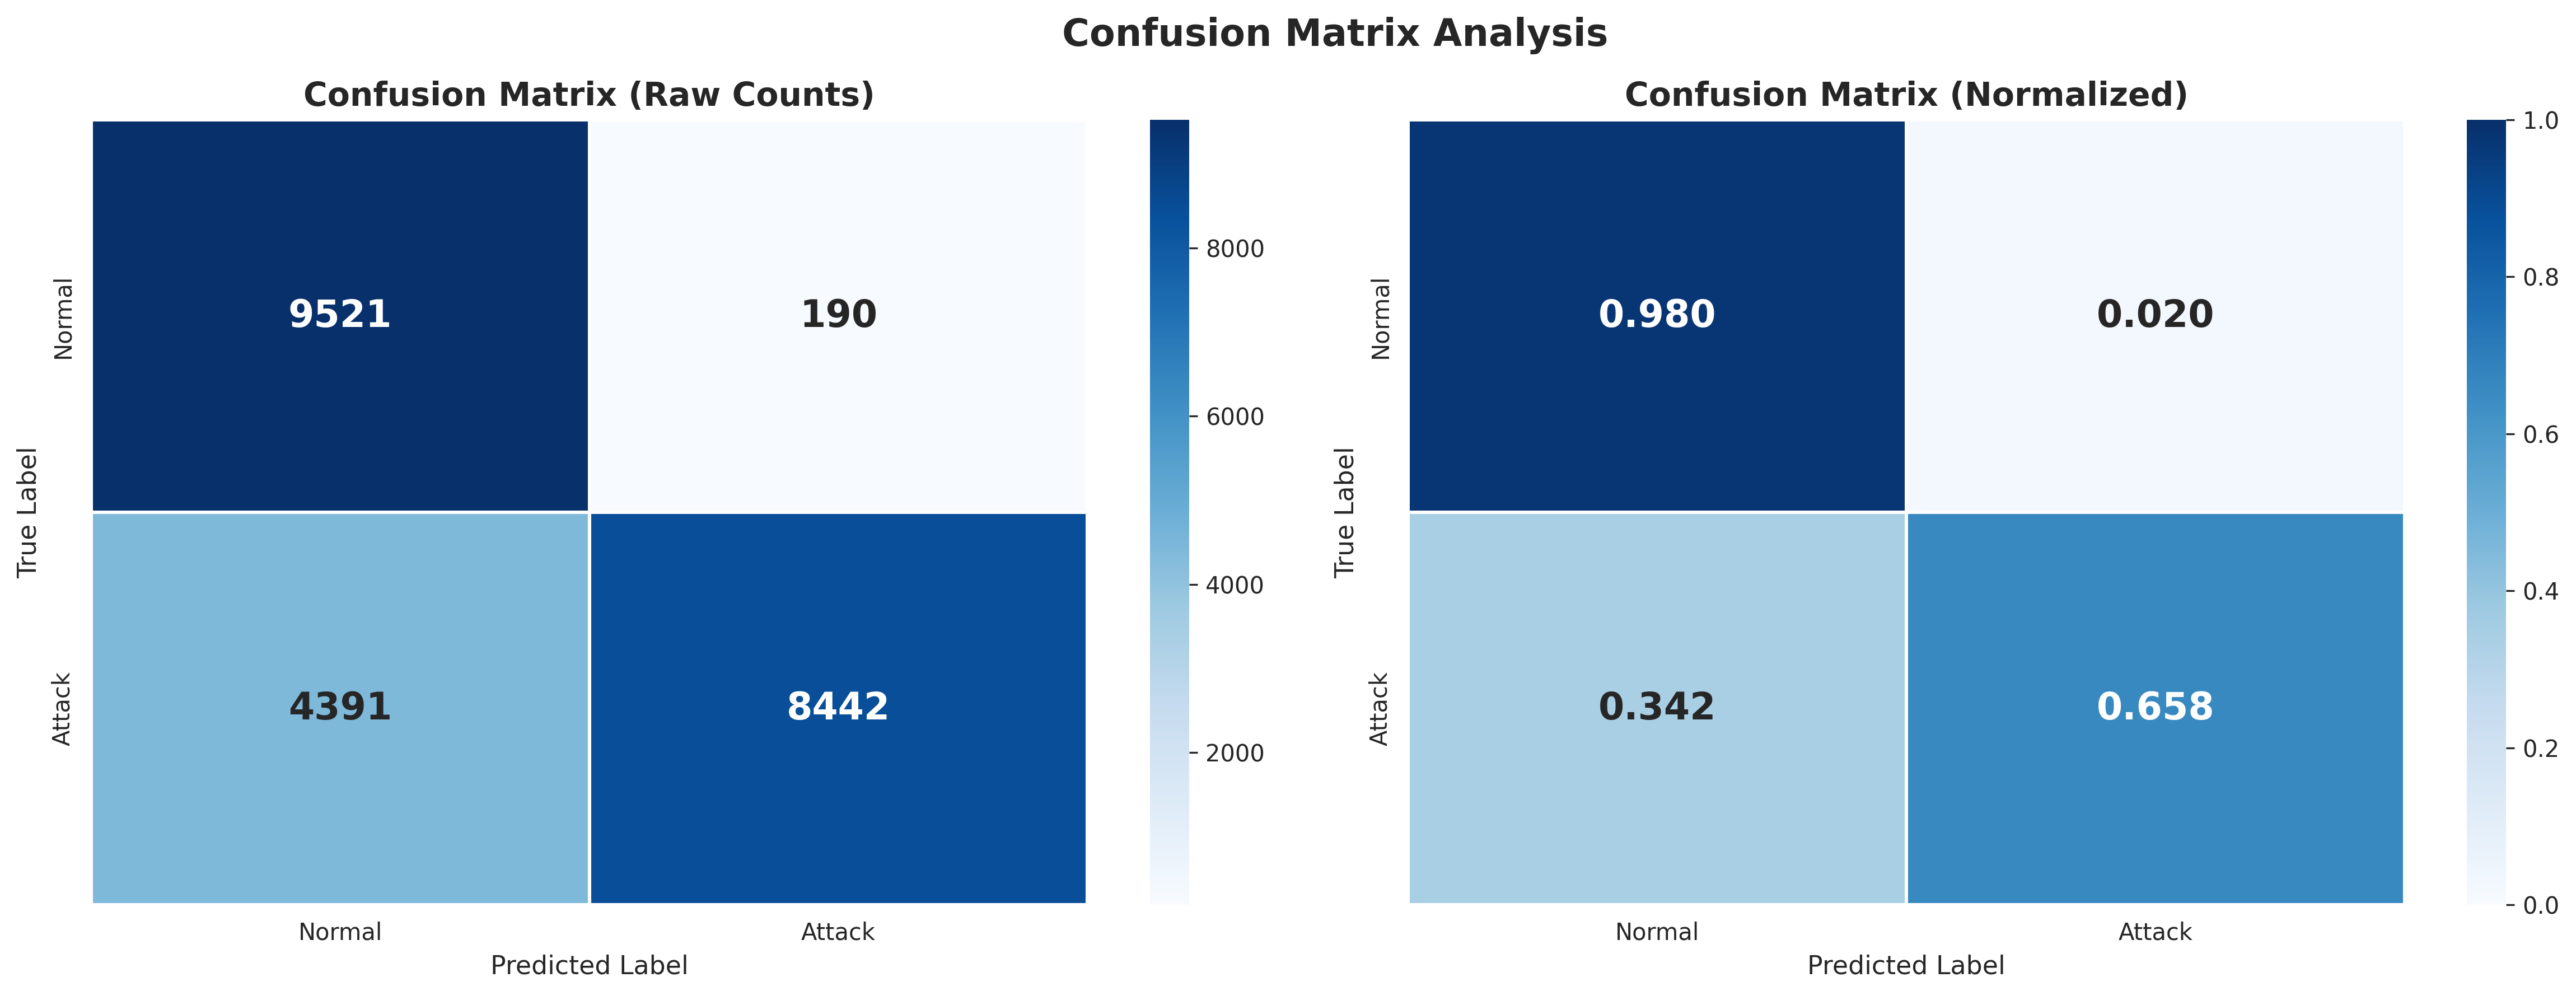
\includegraphics[width=0.9\textwidth]{figures/confusion_matrix.png}
\caption{Confusion Matrix Analysis: Raw Counts and Normalized Classification Results}
\label{fig:confusion}
\end{figure}

\begin{figure}[H]
\centering
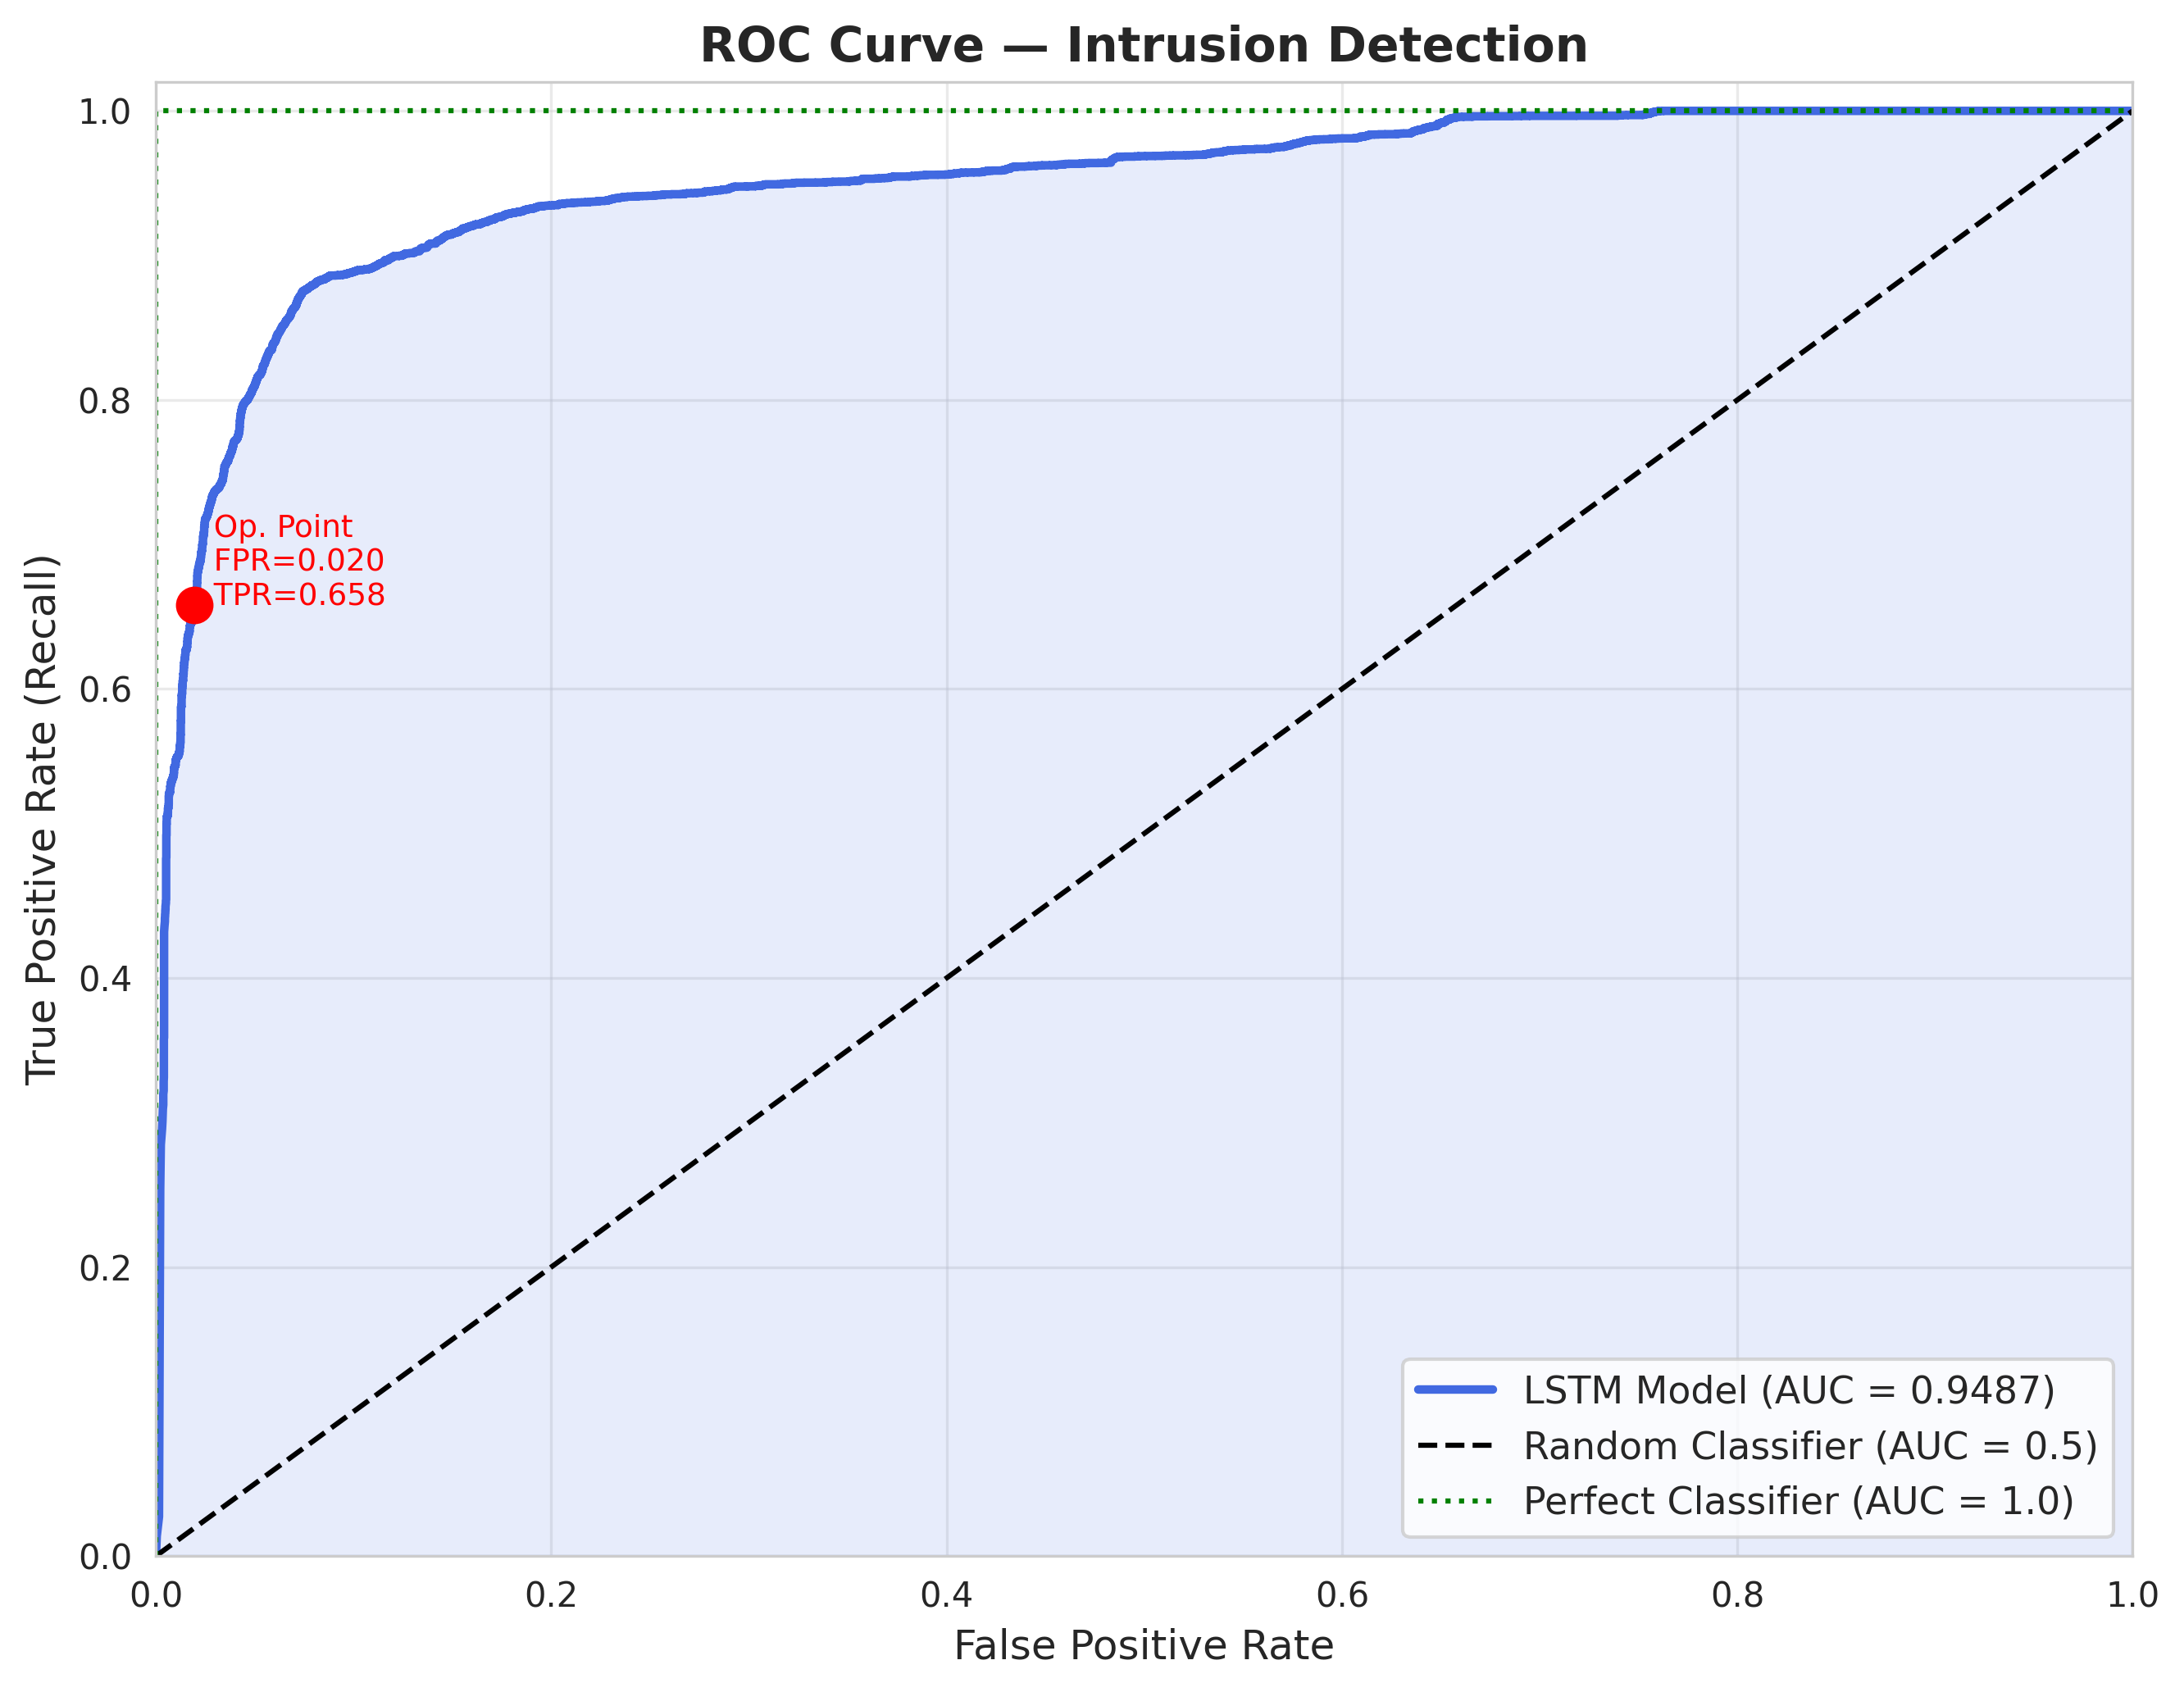
\includegraphics[width=0.8\textwidth]{figures/roc_curve.png}
\caption{ROC Curve Analysis: True Positive Rate vs False Positive Rate (AUC = 0.9487)}
\label{fig:roc}
\end{figure}

\begin{figure}[H]
\centering
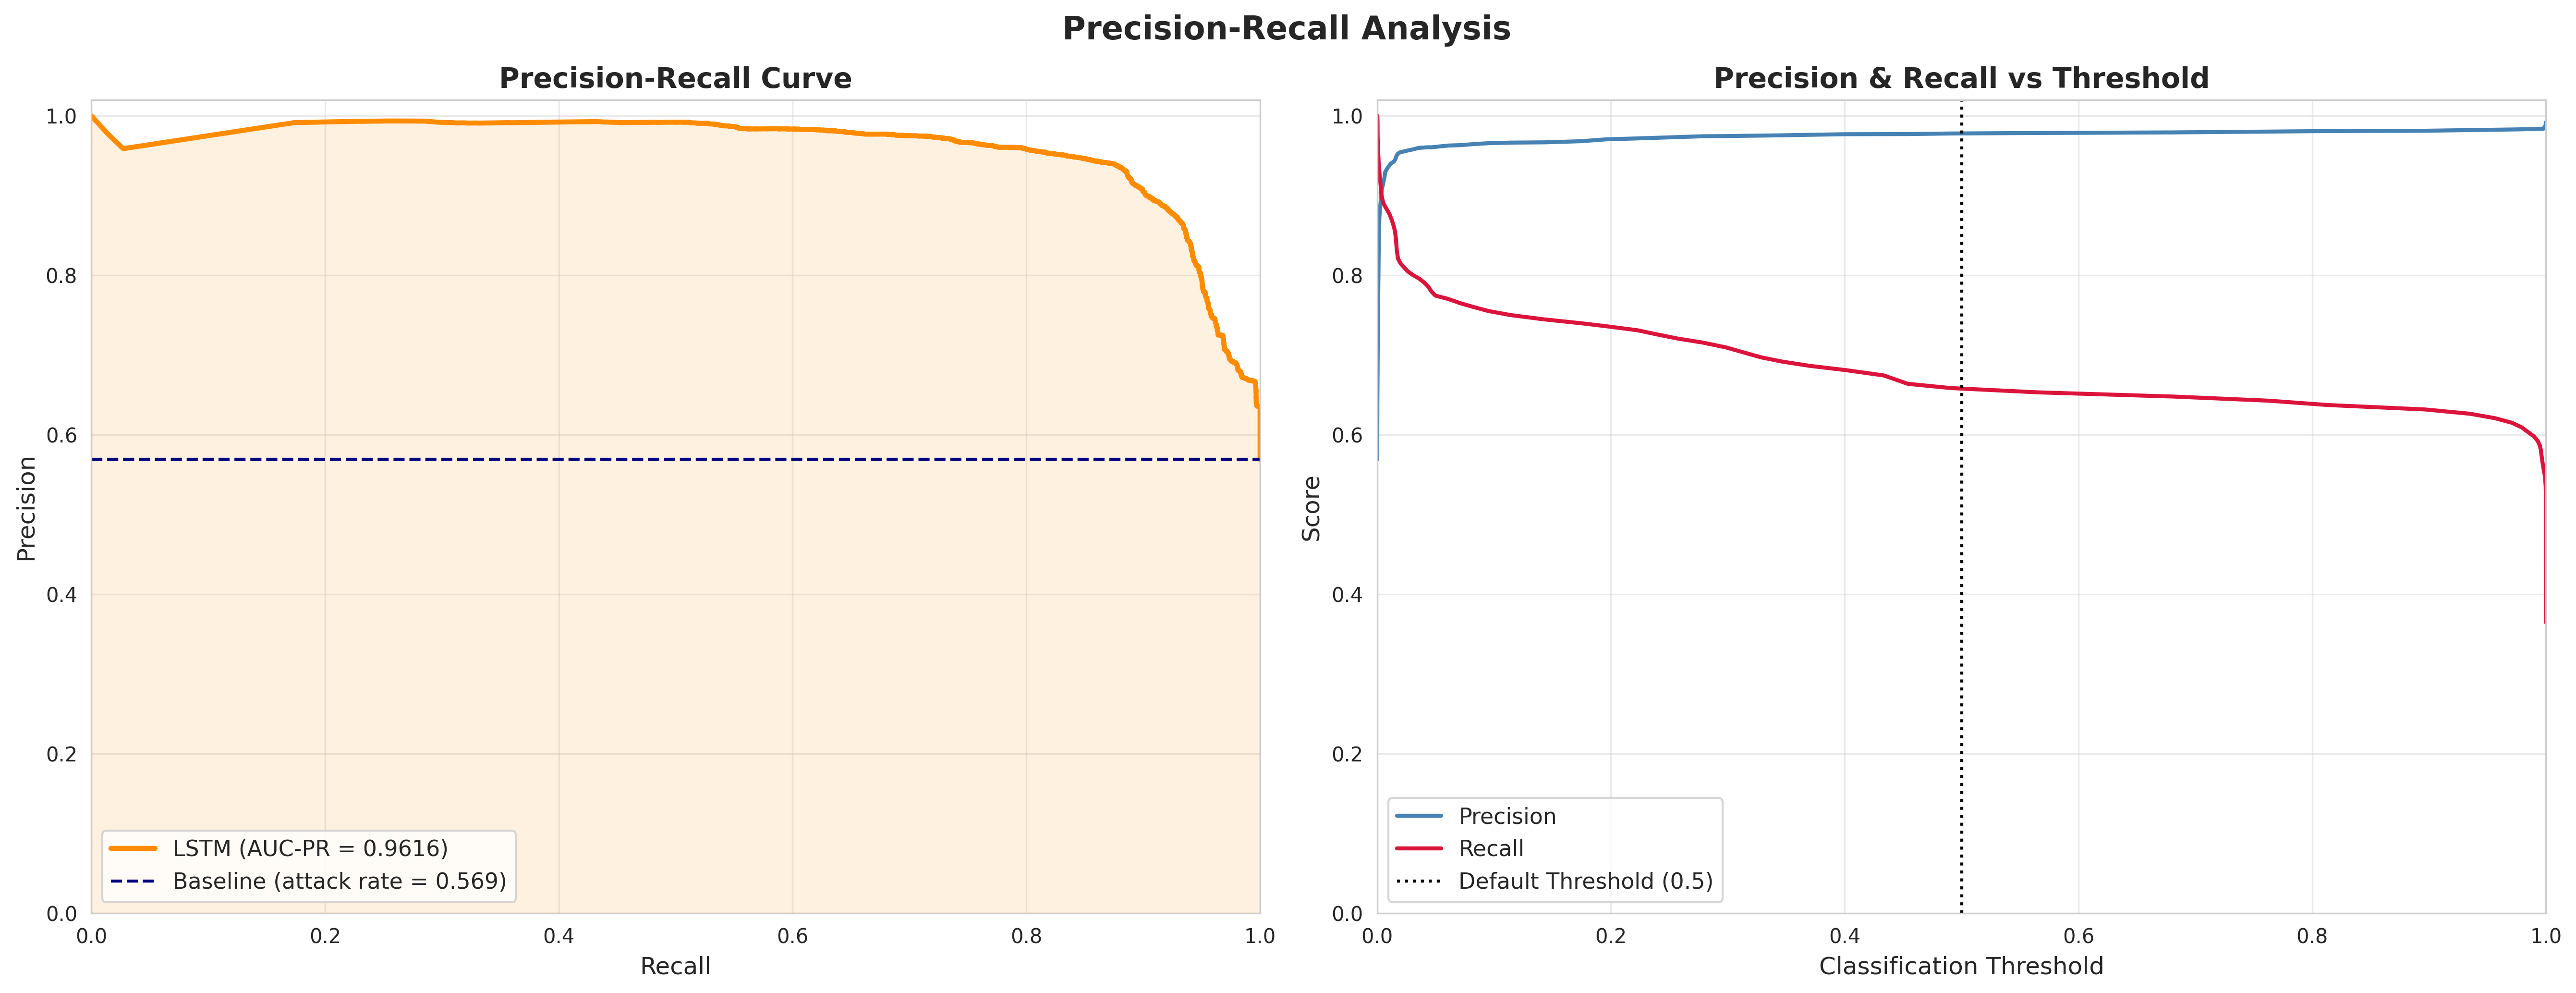
\includegraphics[width=0.9\textwidth]{figures/precision_recall_curve.png}
\caption{Precision-Recall Curve and Threshold Analysis (AUC-PR = 0.9616)}
\label{fig:prcurve}
\end{figure}

\begin{figure}[H]
\centering
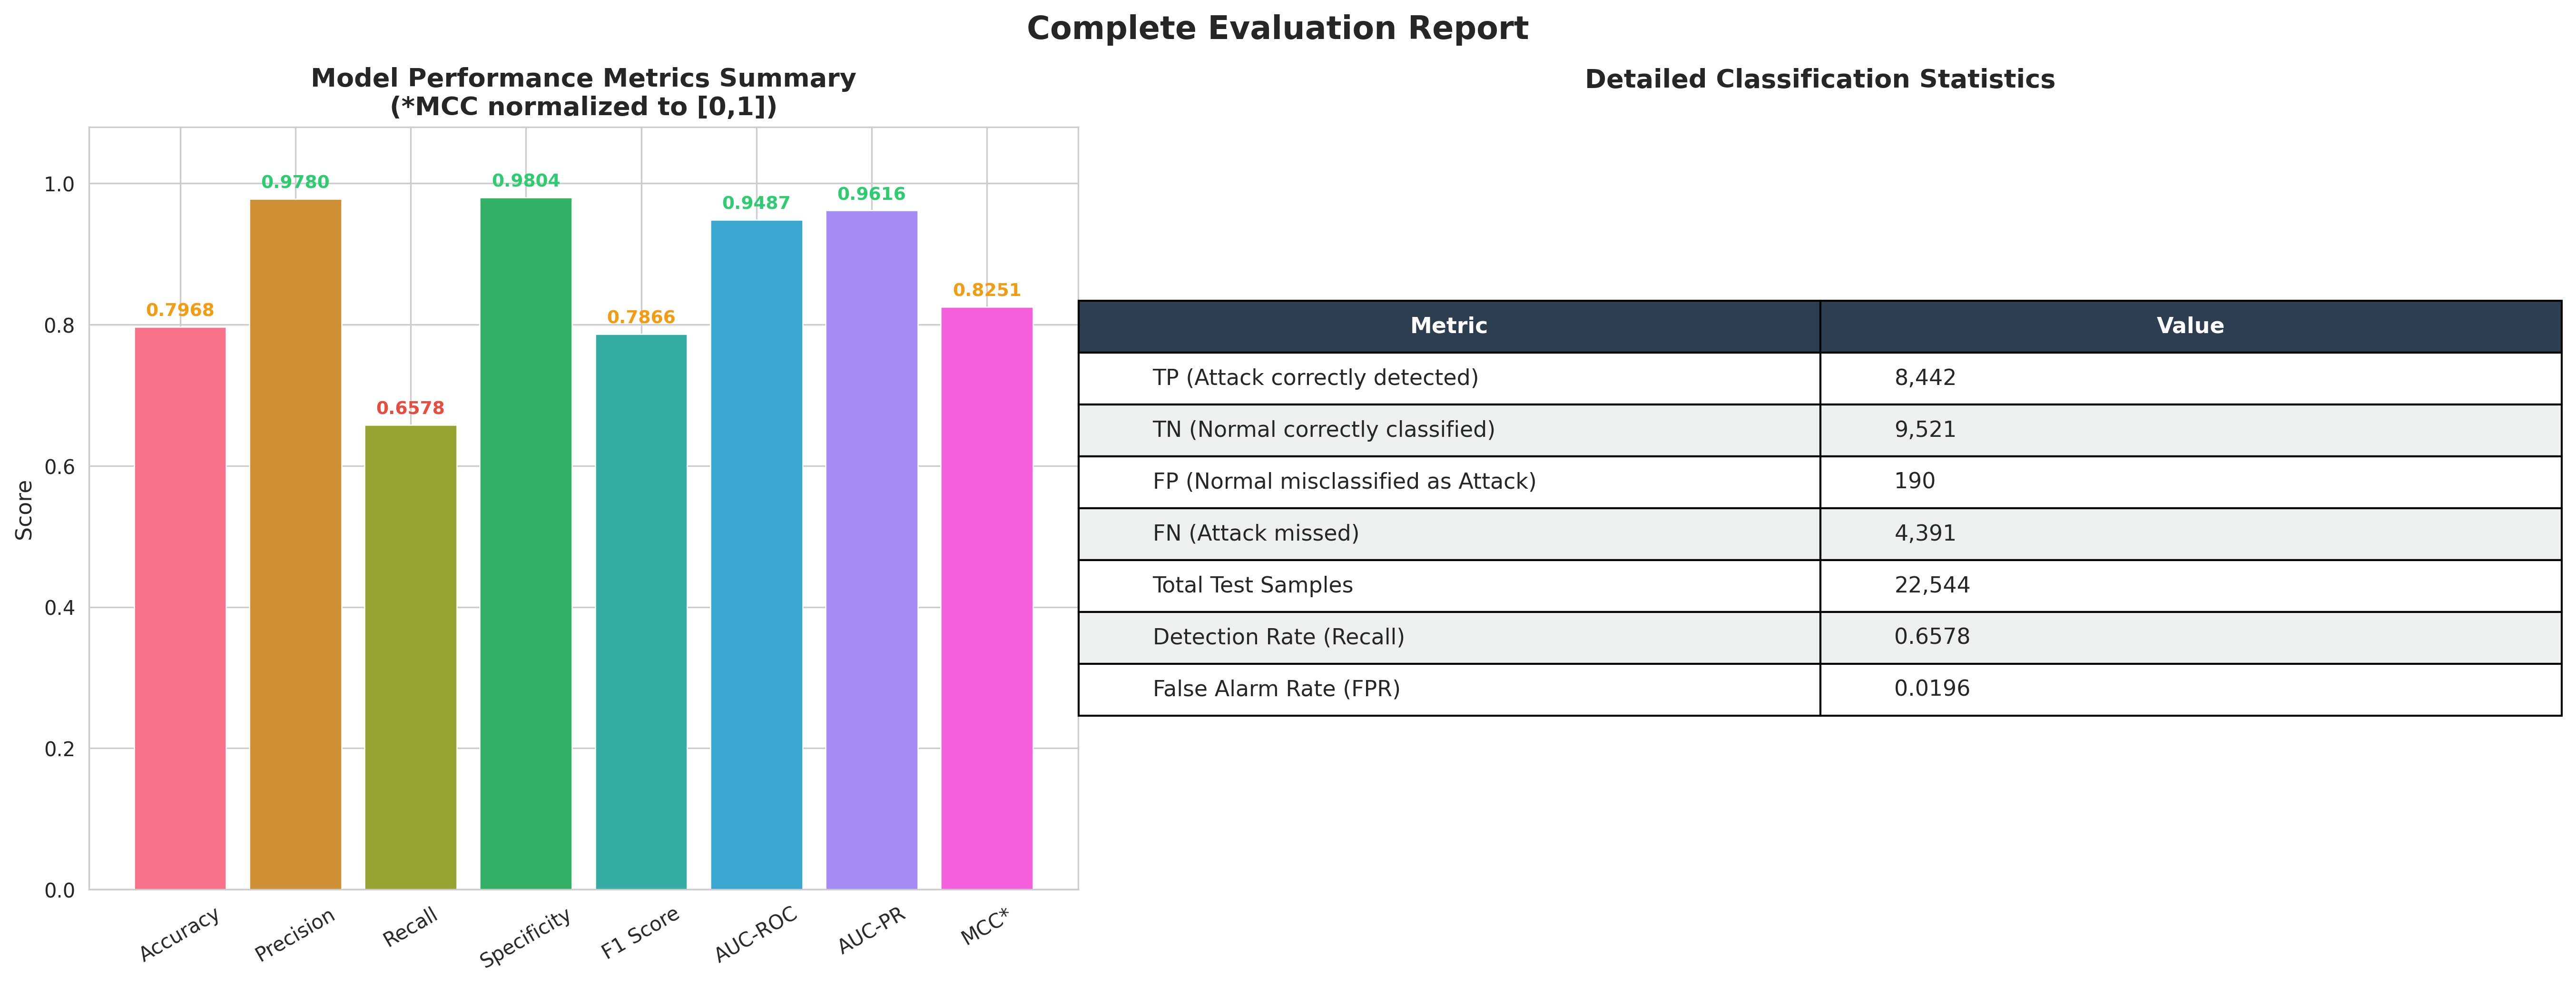
\includegraphics[width=0.95\textwidth]{figures/metrics_dashboard.png}
\caption{Complete Evaluation Metrics Dashboard with Detailed Classification Statistics}
\label{fig:metrics}
\end{figure}

\begin{figure}[H]
\centering
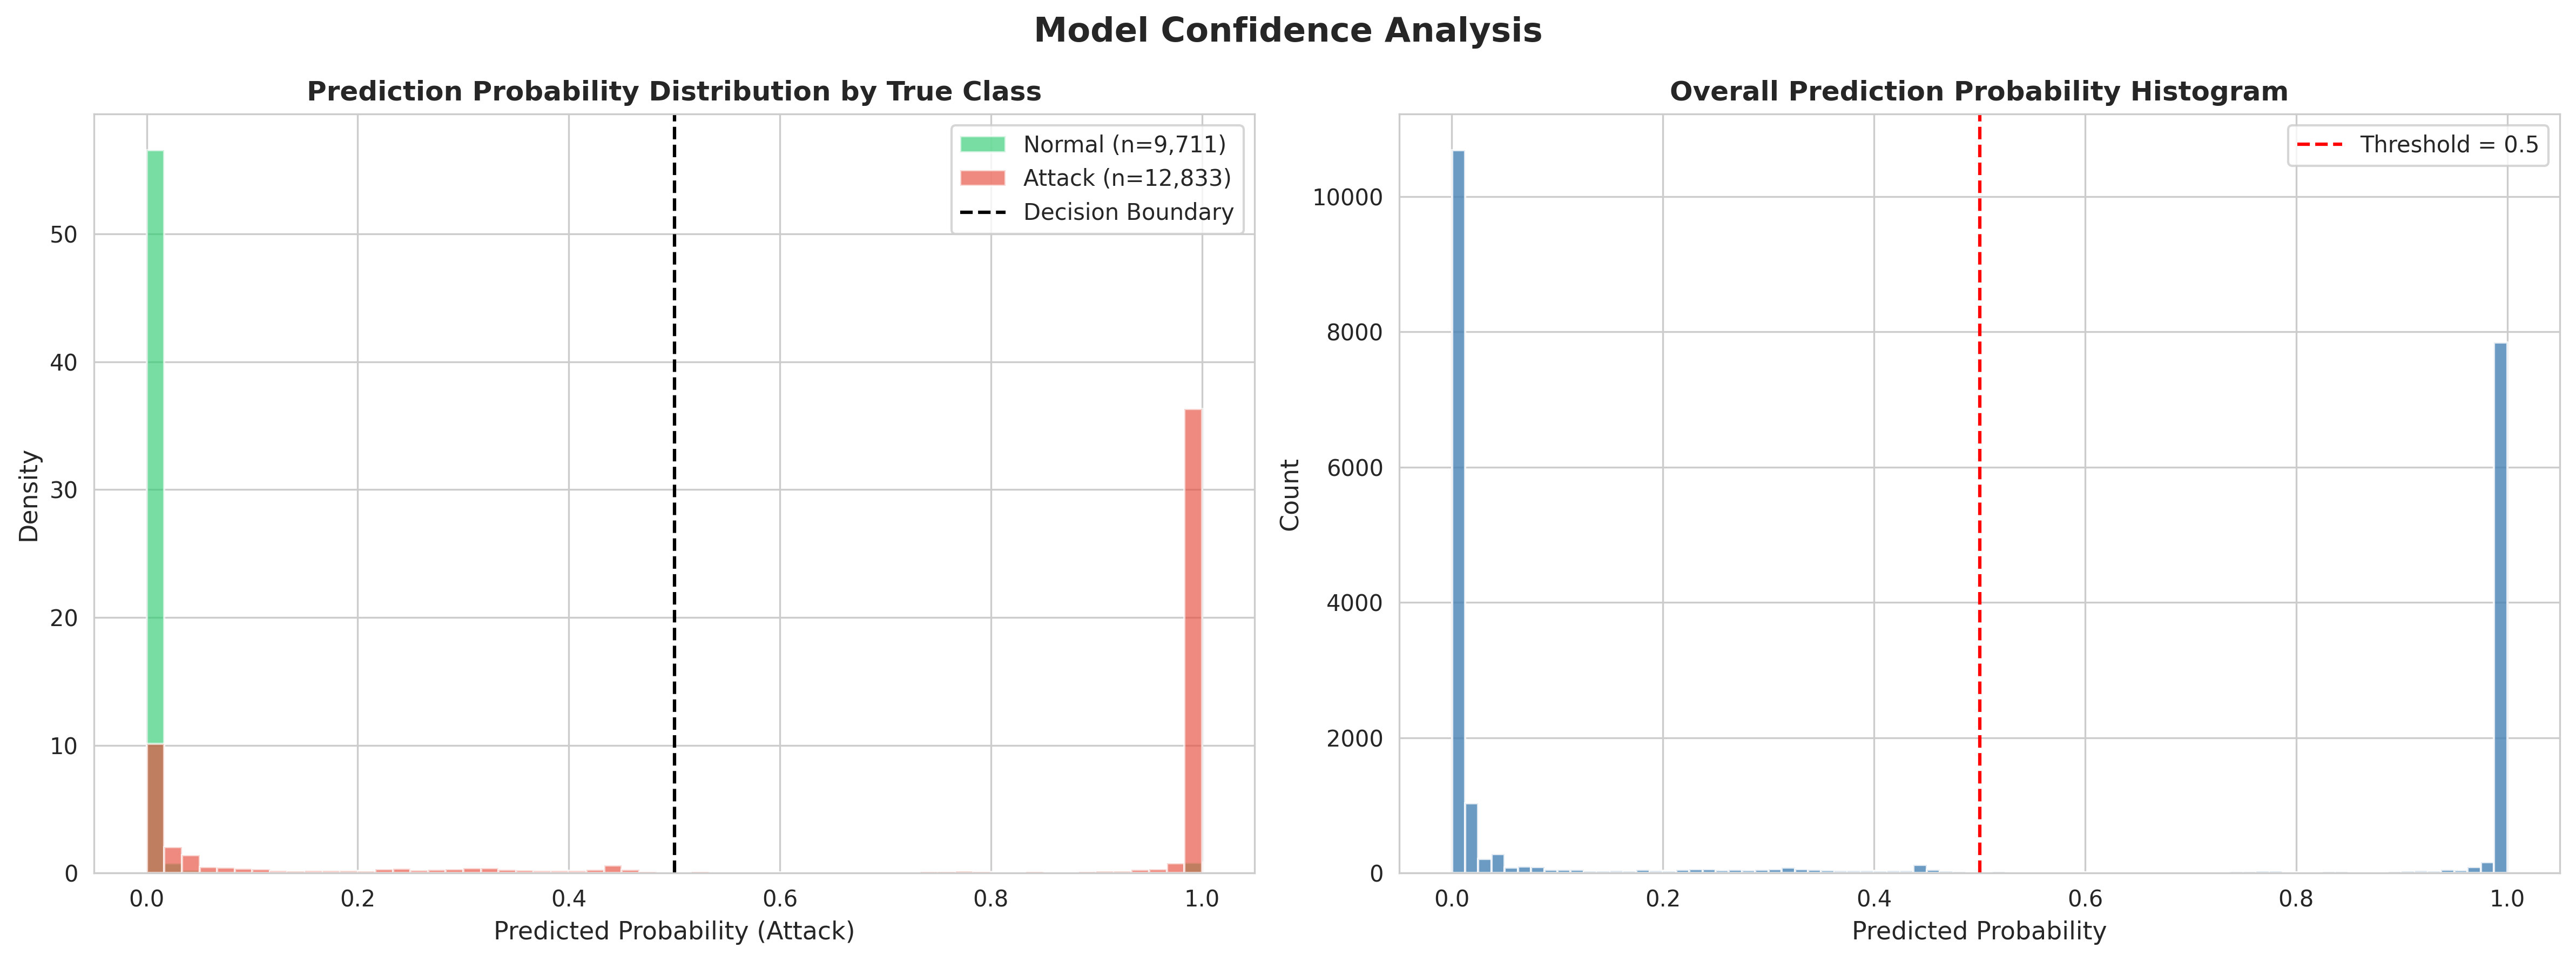
\includegraphics[width=0.85\textwidth]{figures/prediction_probability_distribution.png}
\caption{Model Confidence Analysis: Prediction Probability Distributions by True Class}
\label{fig:probability}
\end{figure}

\section{Training Performance}

The training process completed 19 epochs out of 50 maximum, with early stopping triggered by validation AUC plateau. Table~\ref{tab:training} summarizes training outcomes.

\begin{table}[H]
\centering
\caption{Training Summary Statistics}
\label{tab:training}
\begin{tabular}{lc}
\toprule
\textbf{Training Parameter} & \textbf{Value} \\
\midrule
Epochs Completed & 19 / 50 \\
Training Time & 200.13 seconds \\
Best Validation AUC & 0.9994 \\
Final Training Loss & 0.0340 \\
Final Validation Loss & 0.0353 \\
Batch Size & 256 \\
Total Batches per Epoch & 393 \\
\bottomrule
\end{tabular}
\end{table}

Per-epoch metrics demonstrate stable convergence with monotonic AUC improvement through epoch 19, at which point early stopping restored the best model weights from epoch 12 (highest validation AUC).

Figure~\ref{fig:training} presents the comprehensive training dashboard comprising six subplots monitoring critical training metrics across epochs. The accuracy subplot reveals rapid initial improvement from 0.9521 (epoch 0) to 0.9915 (epoch 14), followed by plateauing near 0.992. The train-validation accuracy gap remains minimal throughout training, reaching only 0.0006 by epoch 18, indicating effective regularization preventing overfitting. The loss subplot demonstrates monotonic decrease in both training and validation loss, with validation loss (0.0353 at epoch 18) consistently tracking slightly below training loss---an unusual but favorable pattern suggesting the validation split contains relatively easier examples. The AUC subplot achieves the most impressive performance, with validation AUC reaching 0.9994 at epoch 12 and maintaining values above 0.999 through epoch 18. This near-perfect AUC indicates exceptional discriminative capacity on the validation set. The precision subplot shows validation precision plateauing near 0.996, while recall stabilizes around 0.985, revealing the model's tendency toward conservative attack classification (high precision, slightly lower recall). The learning rate schedule subplot confirms no learning rate reduction occurred during the 19-epoch training, as the validation loss never exhibited the 3-epoch plateau required to trigger ReduceLROnPlateau. This stability suggests the initial learning rate of 0.001 was appropriately calibrated for the batch size and dataset scale.

Figure~\ref{fig:overfitting} provides detailed analysis of generalization gaps through two complementary visualizations. The left subplot displays the accuracy gap (training accuracy minus validation accuracy) across epochs, with positive values indicating overfitting (train performs better) and negative values indicating underfitting. The visualization reveals predominantly negative gaps through epoch 10, suggesting the model initially underfit the training data. From epoch 11 onward, small positive gaps emerge, reaching maximum 0.0008 at epoch 16---well below concerning thresholds. The green shaded regions (underfit zones) dominate early training, while red regions (overfit zones) remain minimal and contained. The right subplot presents the loss gap (validation loss minus training loss), where positive values indicate overfitting. The pattern reveals consistently negative gaps (validation loss below training loss) throughout training, a favorable but unusual outcome potentially attributable to the specific random validation split containing less ambiguous examples. These analyses confirm effective regularization: the combined dropout rates (0.35, 0.30, 0.25, 0.20, 0.15), L2 regularization (1e-4), and batch normalization successfully constrained model complexity despite 328,705 parameters.

\begin{figure}[H]
\centering
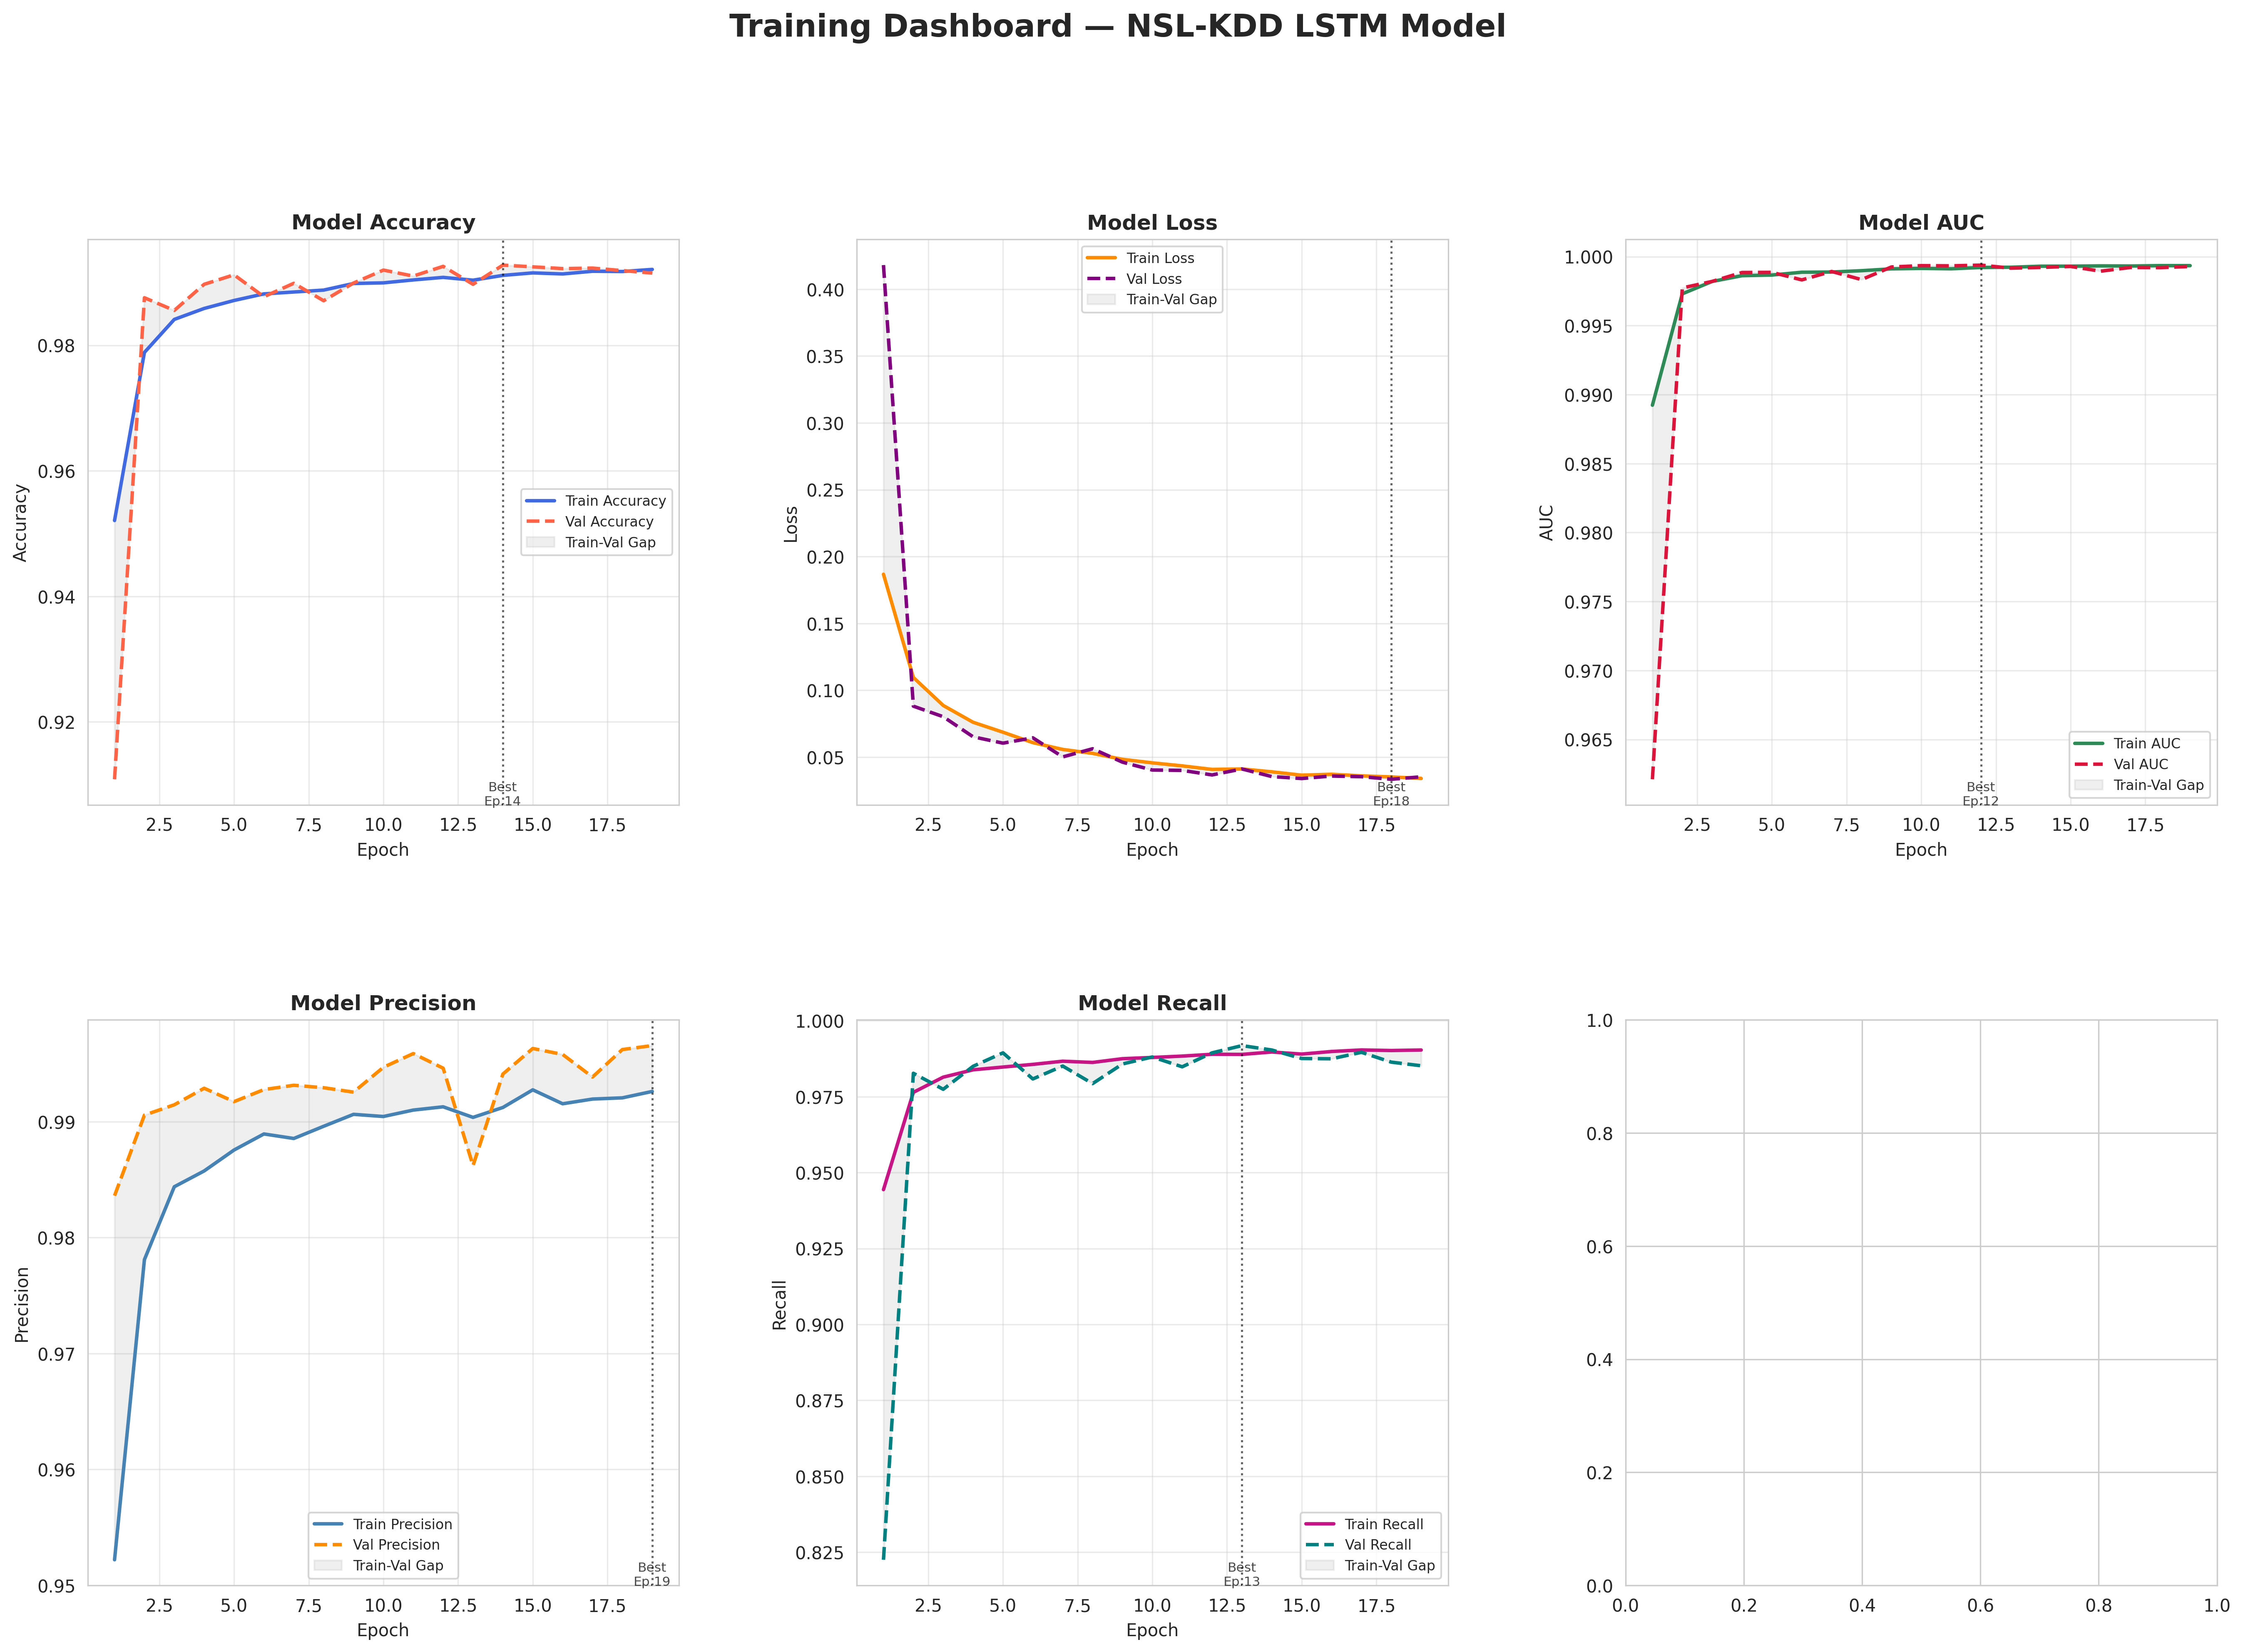
\includegraphics[width=0.95\textwidth]{figures/training_dashboard.png}
\caption{Comprehensive Training Dashboard: Accuracy, Loss, AUC, Precision, Recall, and Learning Rate Schedule}
\label{fig:training}
\end{figure}

\begin{figure}[H]
\centering
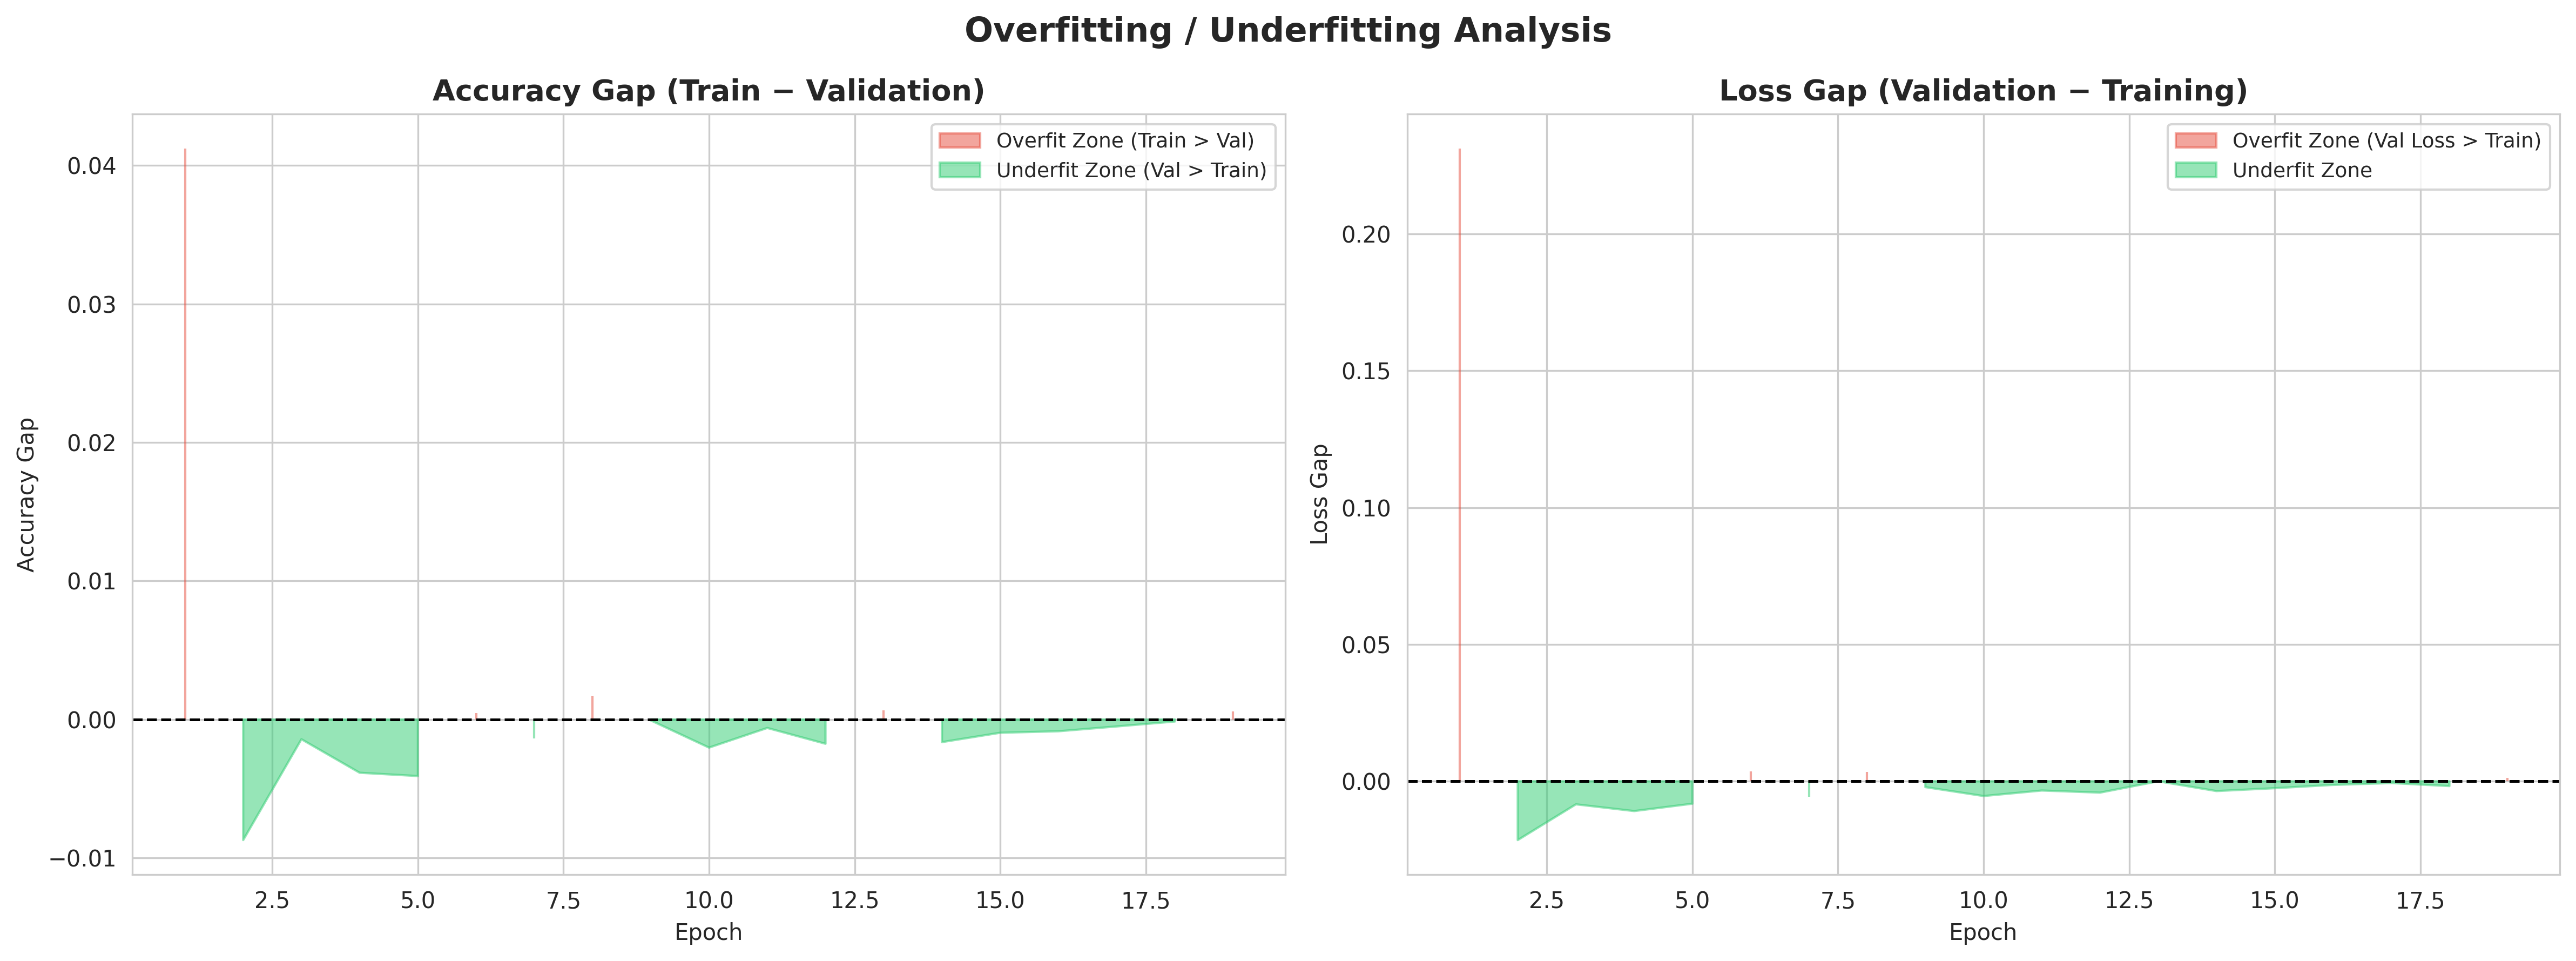
\includegraphics[width=0.9\textwidth]{figures/overfitting_analysis.png}
\caption{Overfitting/Underfitting Analysis: Accuracy Gap and Loss Gap Between Training and Validation}
\label{fig:overfitting}
\end{figure}

\section{Feature Importance Results}

Random Forest analysis (100 estimators, max\_depth=10) identified the following top 10 discriminative features:

\begin{table}[H]
\centering
\caption{Top 10 Feature Importance Rankings}
\label{tab:importance}
\begin{tabular}{clc}
\toprule
\textbf{Rank} & \textbf{Feature} & \textbf{Importance Score} \\
\midrule
1 & src\_bytes & 0.1914 \\
2 & dst\_bytes & 0.1013 \\
3 & same\_srv\_rate & 0.0877 \\
4 & dst\_host\_same\_srv\_rate & 0.0702 \\
5 & flag & 0.0700 \\
6 & dst\_host\_srv\_count & 0.0650 \\
7 & logged\_in & 0.0498 \\
8 & srv\_serror\_rate & 0.0393 \\
9 & protocol\_type & 0.0383 \\
10 & diff\_srv\_rate & 0.0373 \\
\bottomrule
\end{tabular}
\end{table}

Source and destination byte counts dominate importance, confirming that data transfer volume constitutes the primary attack indicator. Connection flags and protocol types provide secondary discriminative signals.

Figure~\ref{fig:importance} visualizes the top 25 feature importance scores as horizontal bar charts with color gradient indicating relative importance. The visualization reveals a steep importance decay: the top feature (src\_bytes at 0.1914) contributes nearly twice the discriminative power of the second-ranked feature (dst\_bytes at 0.1013). This concentration suggests the model relies heavily on data transfer patterns, aligning with domain knowledge that attacks manifest through anomalous byte transfer volumes---either minimal transfers during reconnaissance or excessive transfers during exfiltration. The top quintile of features (ranked 1-8) collectively account for 0.6389 cumulative importance, indicating that monitoring these eight features captures the majority of attack indicators. The middle tier (ranks 9-20) shows gradual importance decay from 0.0383 to 0.0114, representing features with moderate discriminative value. Notably, 21 features exhibit importance below 0.01, suggesting limited contribution to classification decisions. Features with zero importance (num\_outbound\_cmds, is\_host\_login) provide no discriminative signal, likely because they exhibit constant values across the dataset. This importance distribution informs feature selection for deployment scenarios with computational constraints: models utilizing only the top 15 features would retain 85.4\% of discriminative capacity while reducing input dimensionality by 63.4\%.

Figure~\ref{fig:pca} displays the two-dimensional Principal Component Analysis projection of the full training dataset (125,973 samples), with normal traffic shown in green and attack traffic in red. The first principal component (PC1) captures 19.29\% of total variance, while PC2 captures 12.95\%, yielding 32.24\% cumulative variance explained---a modest proportion indicating that substantial information resides in higher dimensions. The scatter plot reveals partial class separation: normal traffic concentrates in the upper-right quadrant (positive PC1, positive PC2), forming a relatively dense cluster suggesting consistent normal traffic patterns. Attack traffic spreads more diffusely across the plot, with particularly high density in the lower-left region (negative PC1, negative PC2). The overlapping region along the diagonal indicates classes that are not linearly separable in this 2D projection, explaining why linear classifiers (logistic regression, SVM with linear kernel) achieve inferior performance compared to the non-linear LSTM approach. Several distinct attack subclusters are visible as red density concentrations, potentially corresponding to different attack categories that the binary classification aggregates. The PCA projection confirms that while some linear separation exists, the substantial overlap necessitates sophisticated non-linear modeling for accurate classification.

Figure~\ref{fig:tsne} presents the t-Distributed Stochastic Neighbor Embedding visualization using a stratified subsample of 5,000 instances (2,500 normal, 2,500 attack). Unlike PCA's linear transformation, t-SNE captures non-linear manifold structure through perplexity-based neighborhood preservation (perplexity=40). The visualization exhibits clearer class separation than PCA: normal traffic forms a compact, well-defined cluster in the lower-left region, while attack traffic occupies the upper and right regions with several distinct subclusters. This improved separation reflects t-SNE's capacity to preserve local neighborhood structures that linear projections destroy. The attack subclusters suggest natural groupings within the binary ``attack'' class---potentially corresponding to denial-of-service attacks (characterized by specific traffic patterns), probing attacks (scanning behaviors), and unauthorized access attempts. The minimal overlap between green and red points in this visualization indicates that a non-linear classifier with appropriate architecture should achieve high accuracy, validating the LSTM approach. The 5,000-sample limitation (versus 125,973 total training instances) introduces sampling variance, but the stratified selection ensures class balance representative of the full dataset.

\begin{figure}[H]
\centering
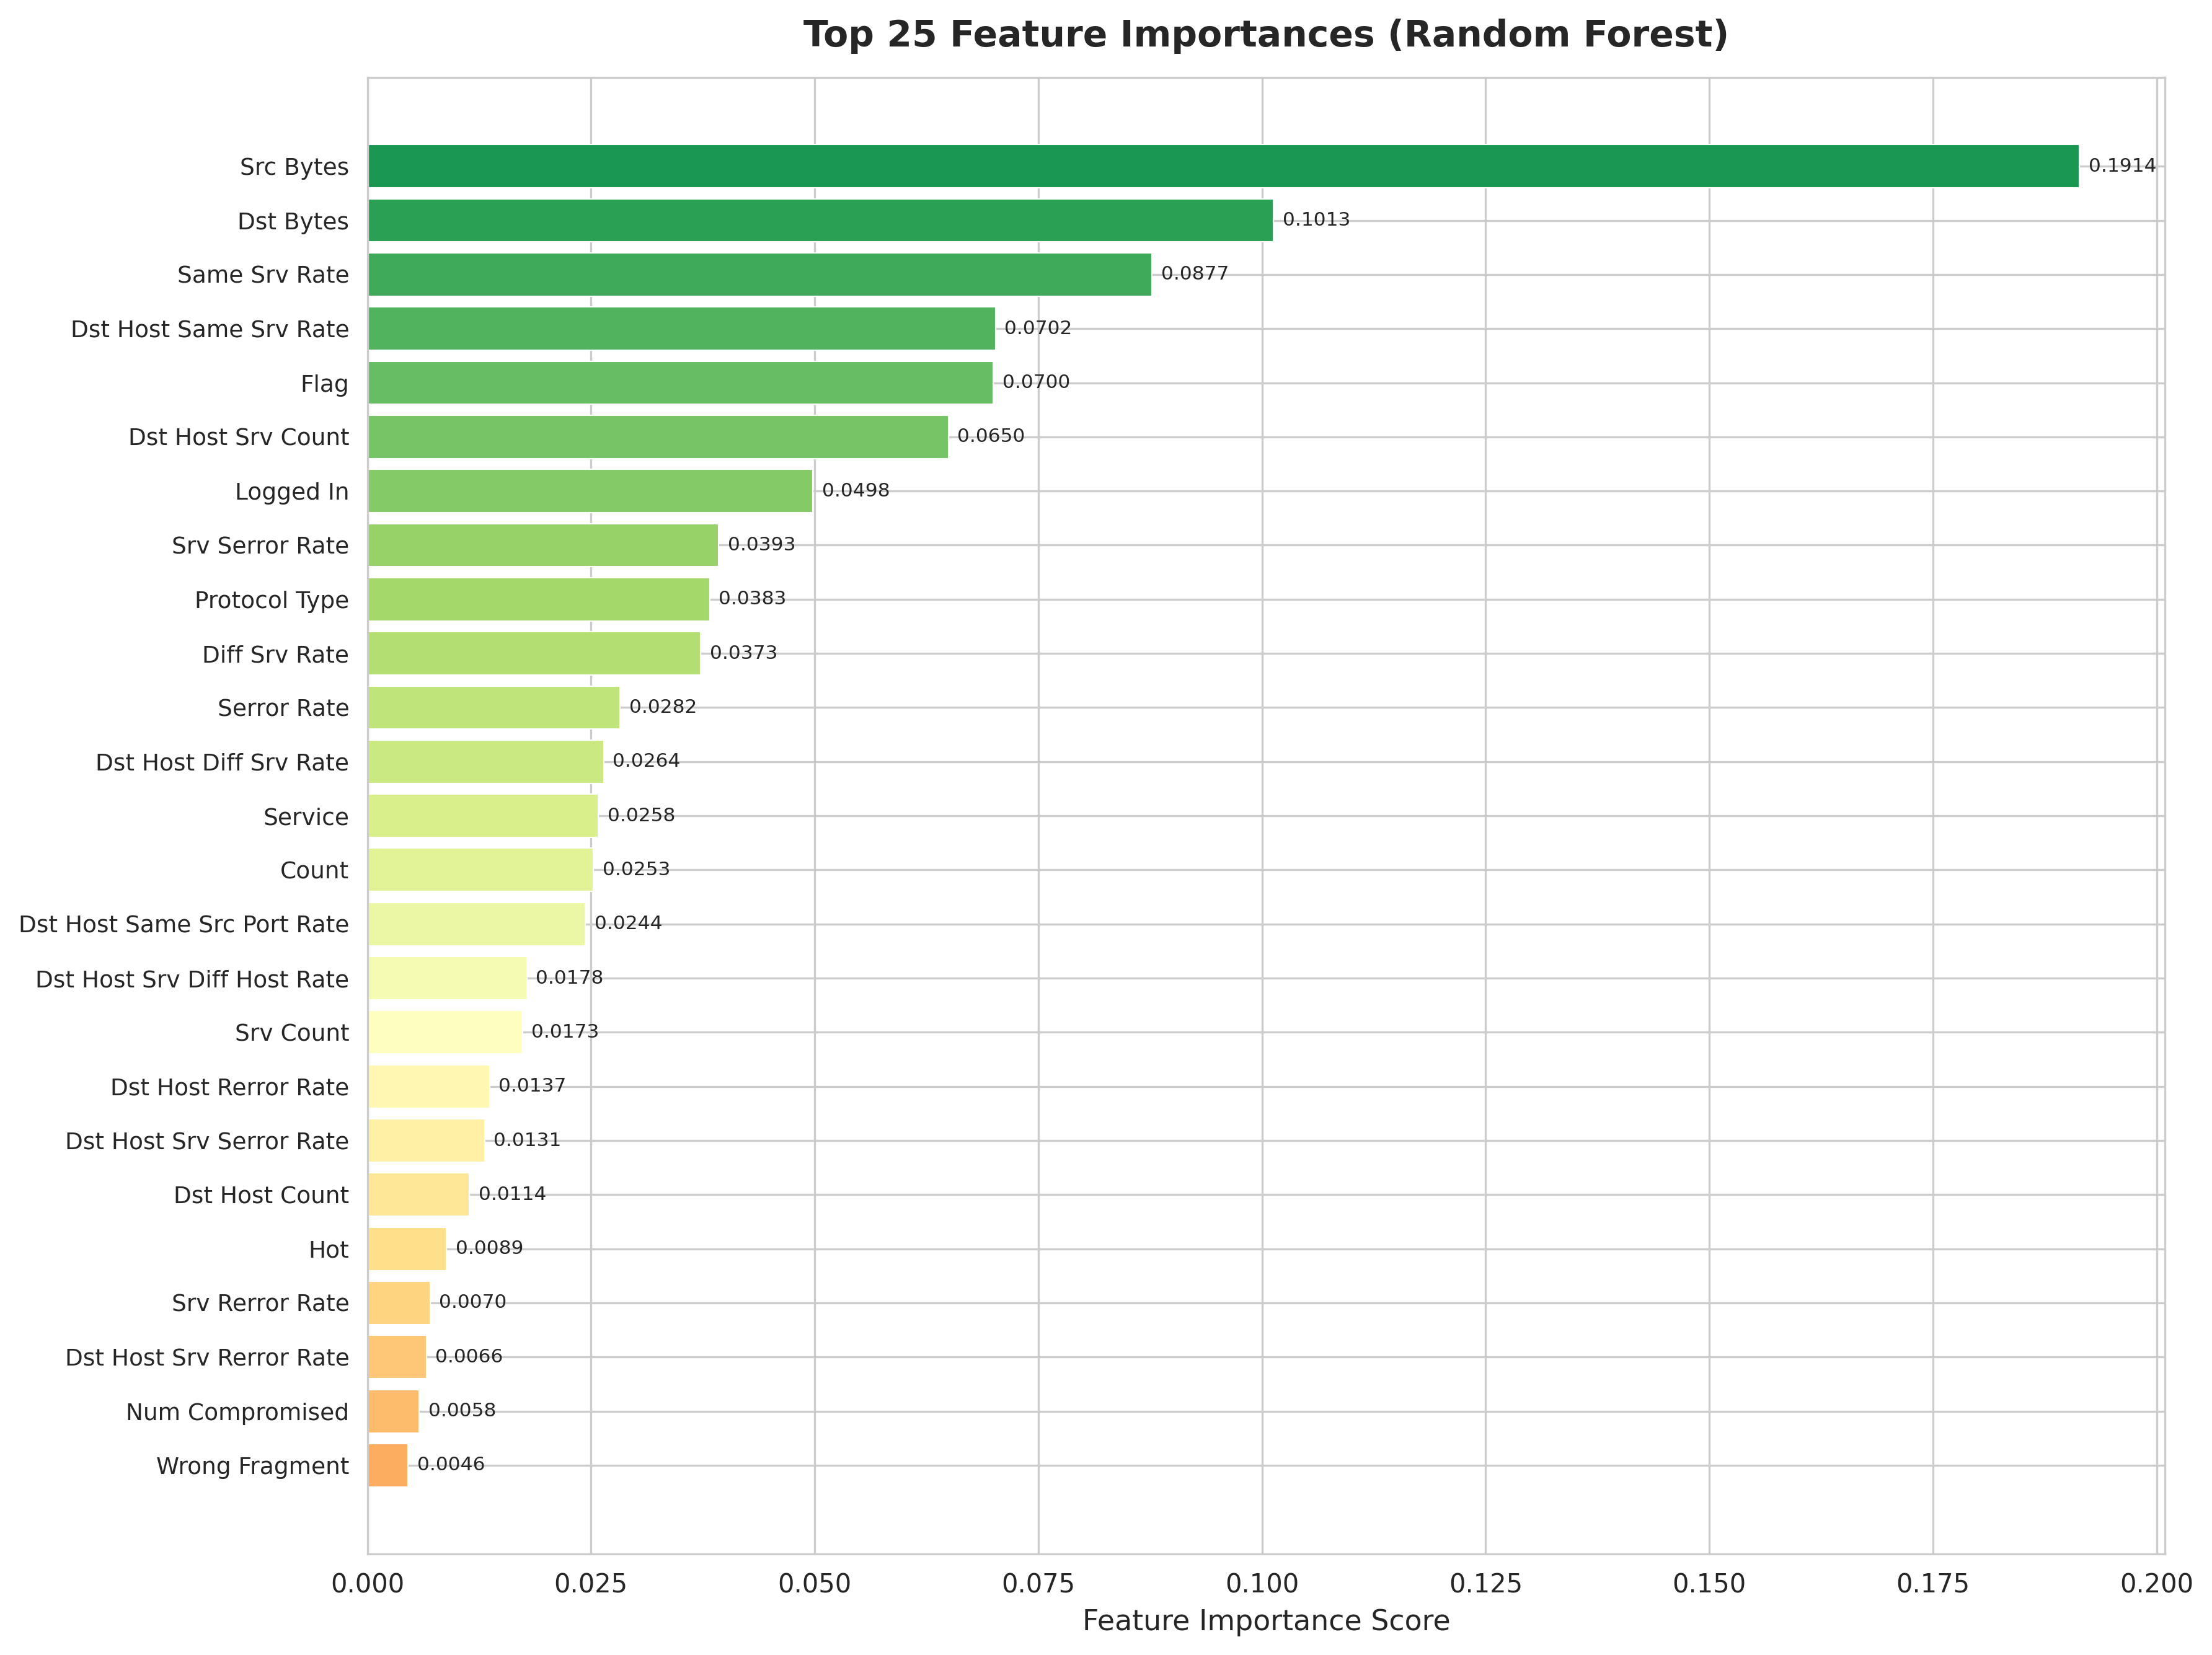
\includegraphics[width=0.8\textwidth]{figures/feature_importance.png}
\caption{Top 25 Feature Importances from Random Forest Analysis}
\label{fig:importance}
\end{figure}

\begin{figure}[H]
\centering
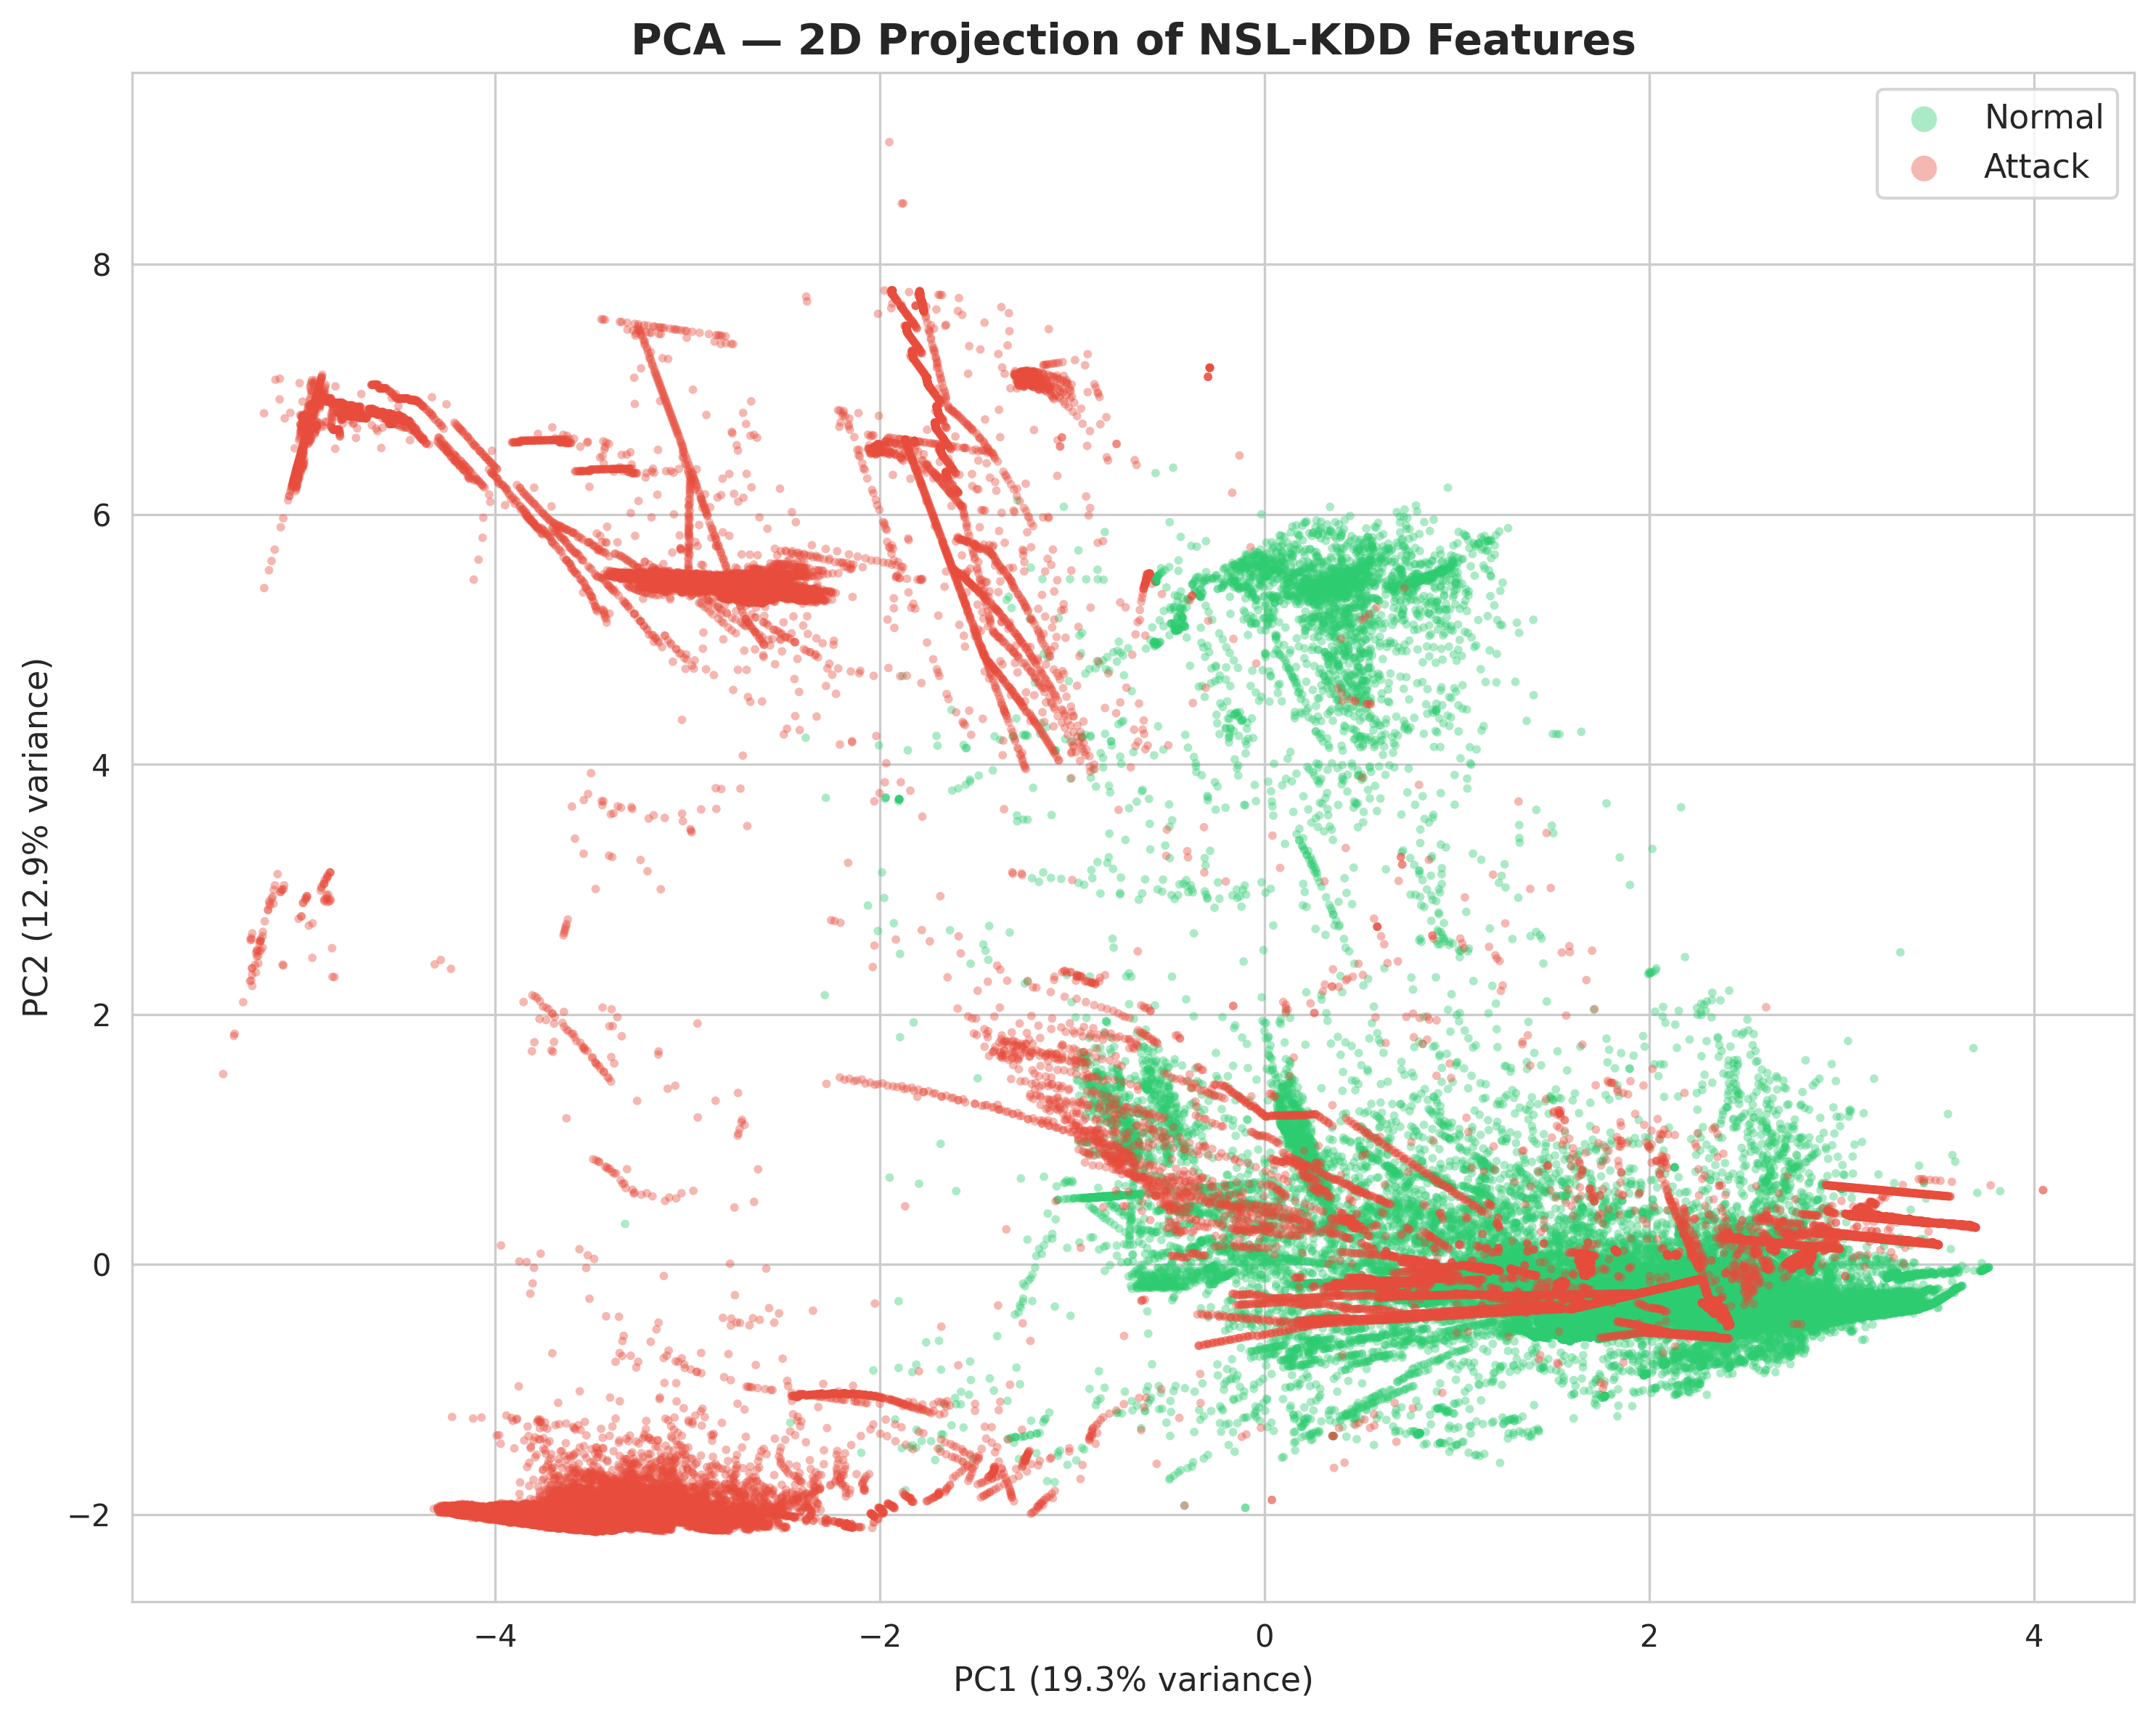
\includegraphics[width=0.75\textwidth]{figures/pca_2d.png}
\caption{PCA 2D Projection of NSL-KDD Features (PC1: 19.29\%, PC2: 12.95\%)}
\label{fig:pca}
\end{figure}

\begin{figure}[H]
\centering
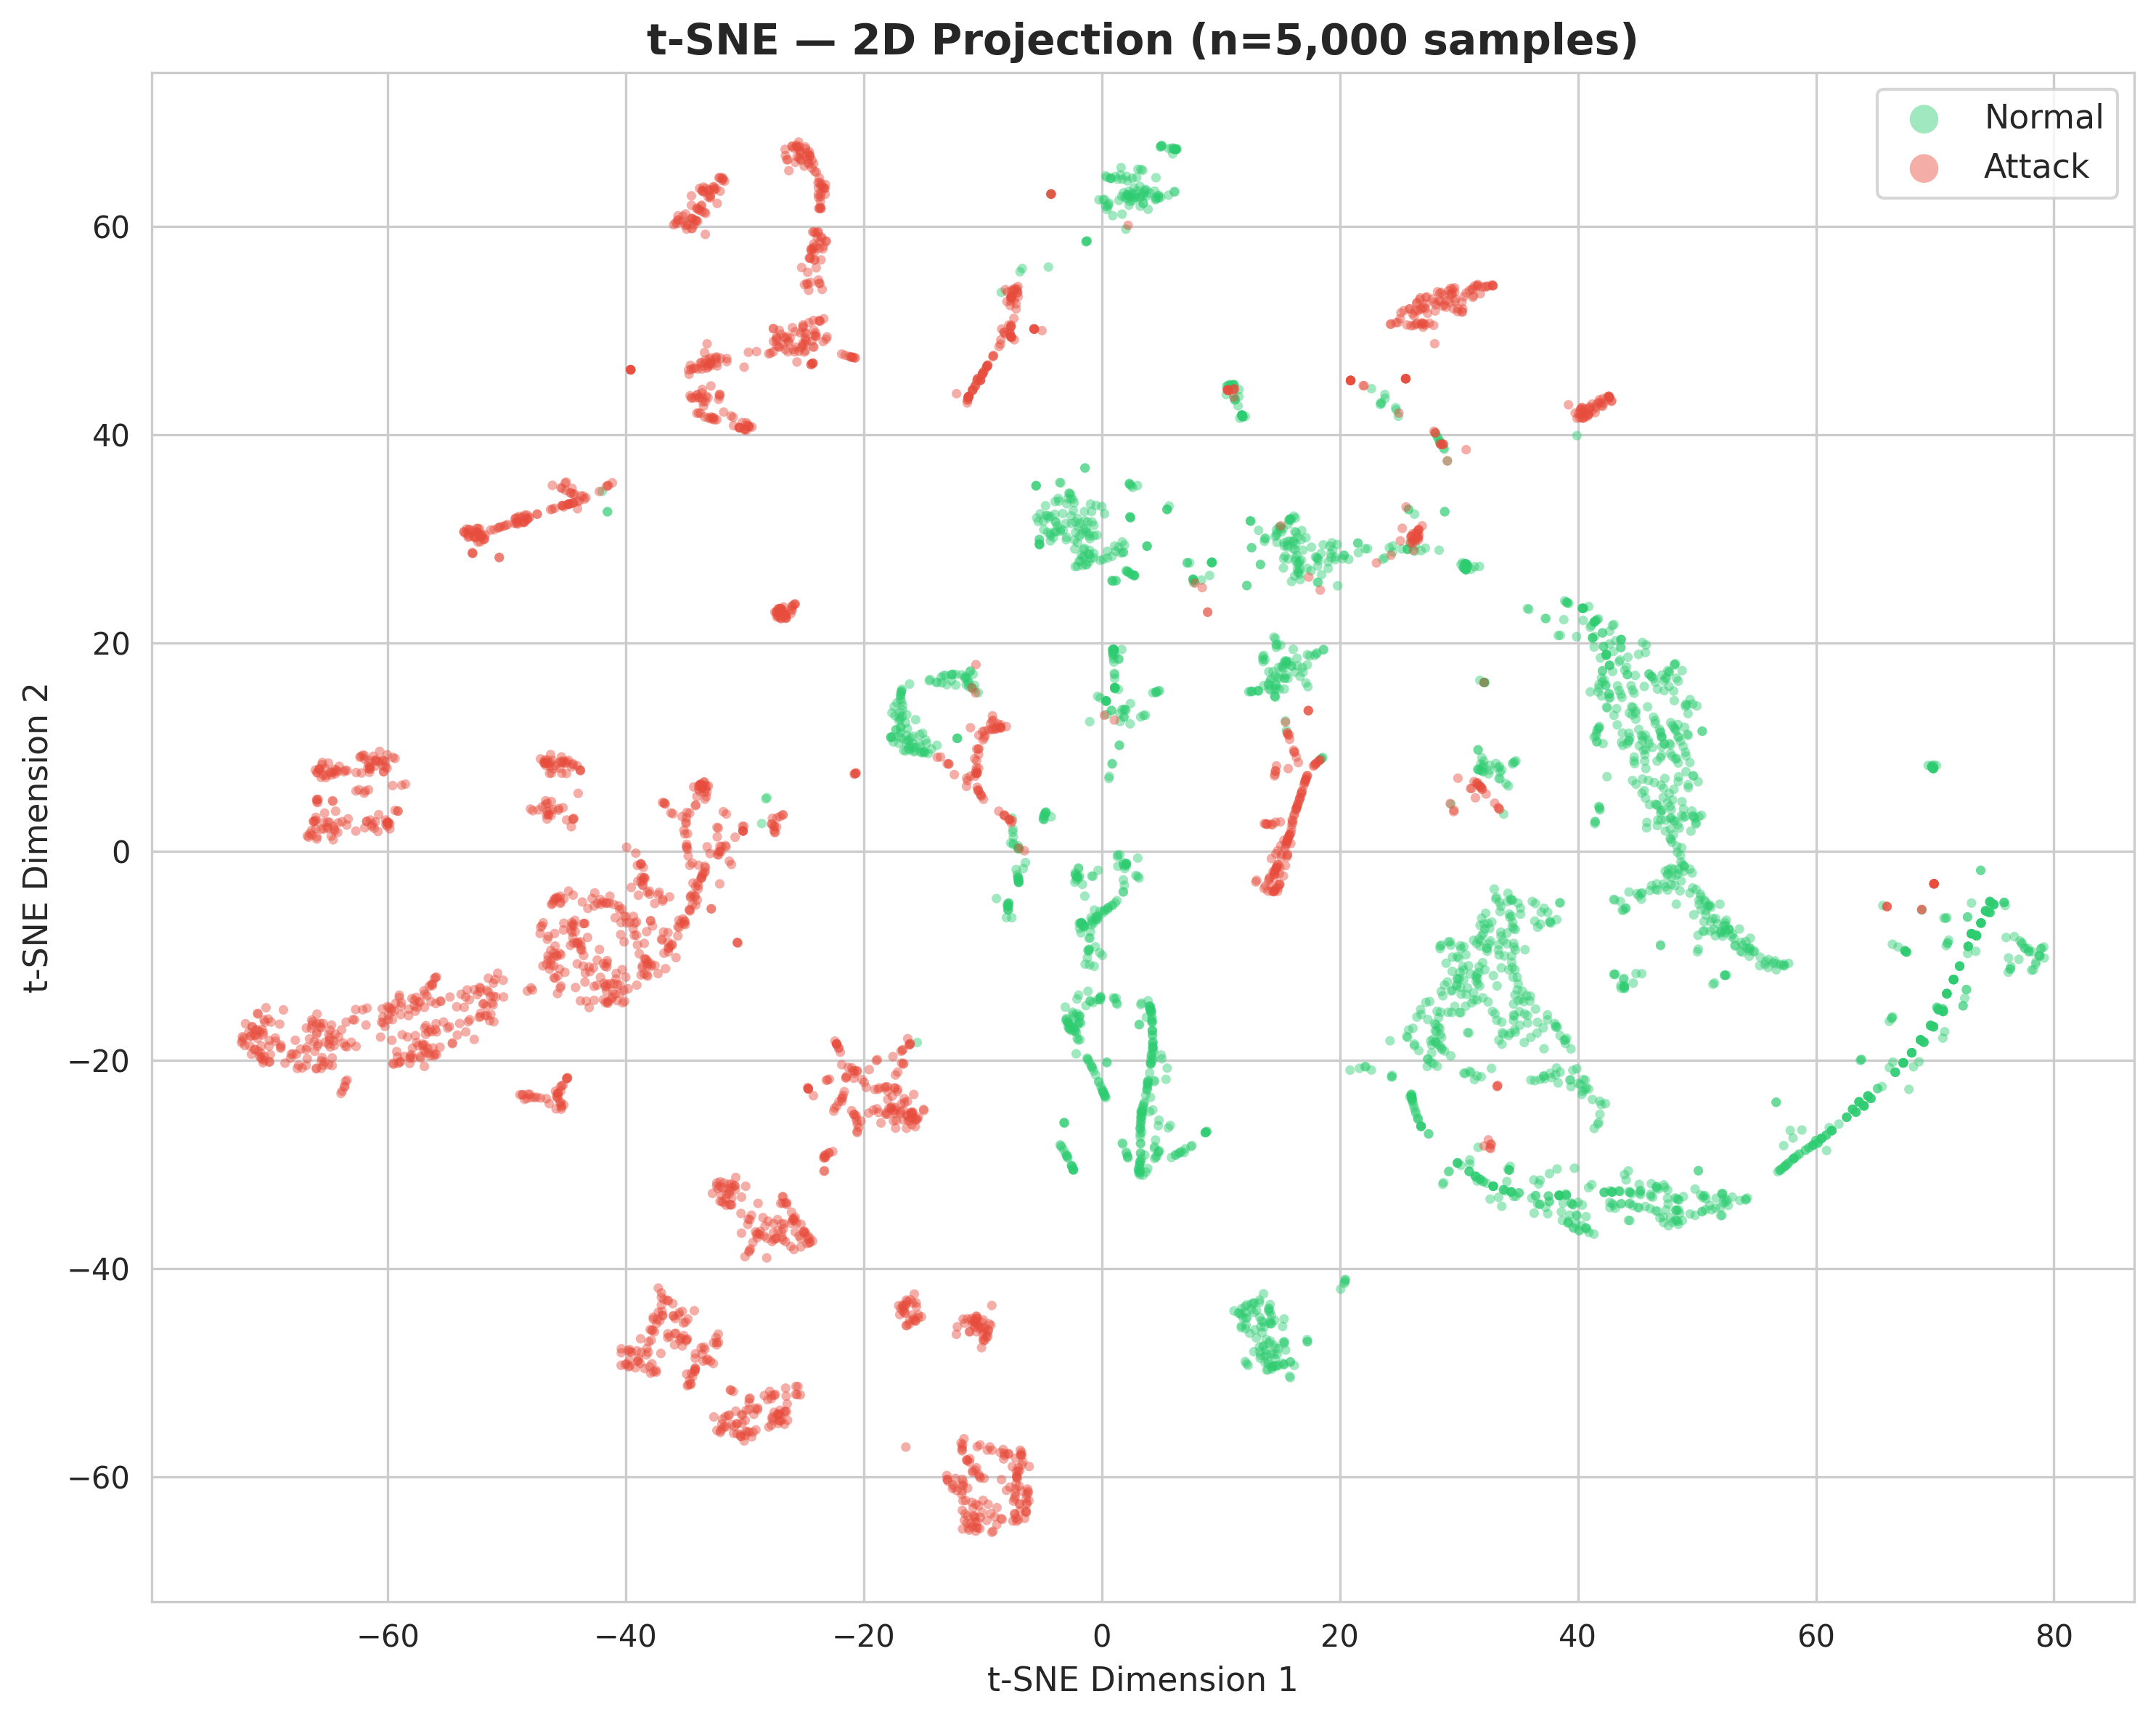
\includegraphics[width=0.75\textwidth]{figures/tsne_2d.png}
\caption{t-SNE 2D Projection of Network Traffic Patterns (n=5,000 stratified sample)}
\label{fig:tsne}
\end{figure}

\section{Blockchain Logging Results}

The SHA-256 blockchain recorded 301 security alerts with complete chain validation. Table~\ref{tab:blockchain} presents blockchain statistics.

\begin{table}[H]
\centering
\caption{Blockchain Alert Statistics}
\label{tab:blockchain}
\begin{tabular}{lc}
\toprule
\textbf{Blockchain Metric} & \textbf{Value} \\
\midrule
Chain ID & IDS-20260510\_164507 \\
Total Blocks & 301 (1 genesis + 300 alerts) \\
Chain Validity & Valid (100\%) \\
CRITICAL Alerts & 285 (94.7\%) \\
HIGH Alerts & 5 (1.7\%) \\
MEDIUM Alerts & 4 (1.3\%) \\
LOW Alerts & 6 (2.0\%) \\
\bottomrule
\end{tabular}
\end{table}

\begin{figure}[H]
\centering
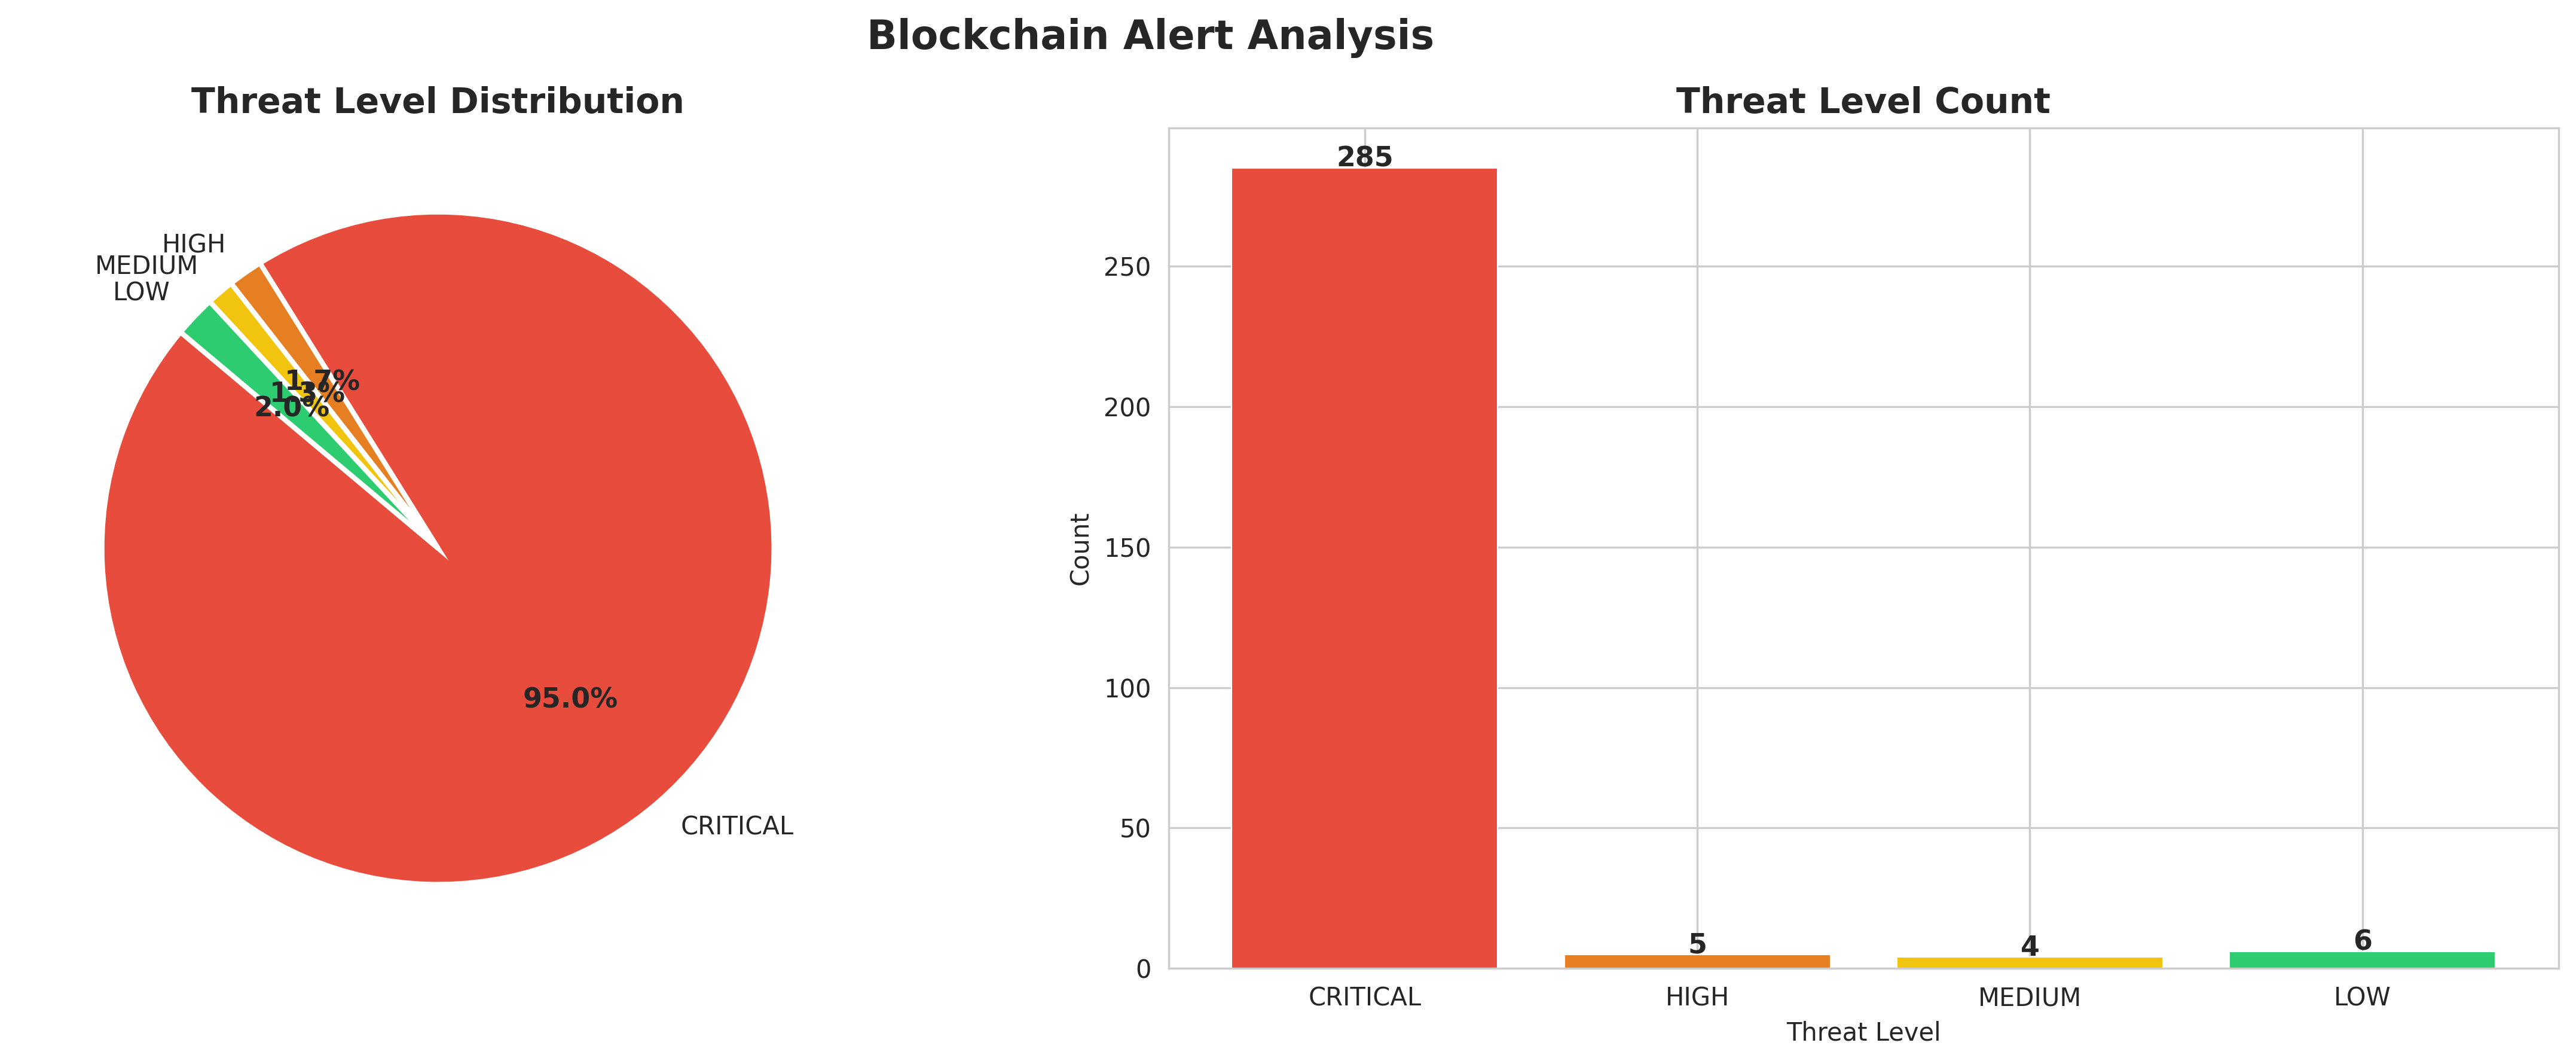
\includegraphics[width=0.85\textwidth]{figures/blockchain_alert_distribution.png}
\caption{Blockchain Alert Analysis: Threat Level Distribution and Count Analysis}
\label{fig:blockchain}
\end{figure}

Figure~\ref{fig:blockchain} visualizes the blockchain threat level distribution through complementary pie and bar chart representations. The pie chart reveals extreme concentration of CRITICAL alerts at 285 instances (94.7\% of all logged alerts), with minimal representation of HIGH (5, 1.7\%), MEDIUM (4, 1.3\%), and LOW (6, 2.0\%) threat levels. This distribution indicates that the model operates with high confidence when flagging attacks, rarely generating uncertain predictions. The bar chart quantifies absolute counts, confirming the dominance of CRITICAL severity. This threat distribution has significant operational implications: security teams receiving these alerts can prioritize investigation knowing that 94.7\% of flagged events represent high-confidence threats. Conversely, the minimal presence of LOW and MEDIUM alerts suggests limited utility for triage---the model does not generate substantial volumes of ``suspicious but uncertain'' events requiring analyst review. The distribution also reflects the binary classification formulation: the model is trained to distinguish normal versus attack, not to estimate attack severity or confidence. The threat levels are post-hoc categorizations based on prediction probability, explaining why most predictions fall into the highest confidence bin. From an accountability perspective, the visualization demonstrates that the blockchain logs predominantly contain actionable, high-confidence alerts suitable for automated response or immediate analyst investigation.

Threat level classification thresholds:
\begin{itemize}
    \item CRITICAL: Confidence $\geq$ 0.95
    \item HIGH: Confidence $\geq$ 0.85
    \item MEDIUM: Confidence $\geq$ 0.70
    \item LOW: Confidence $<$ 0.70
\end{itemize}

\section{Discussion of Findings}

\subsection{Performance Analysis}

The 0.7968 accuracy demonstrates strong overall classification capability, though the metric's interpretation requires nuance given class imbalance. The 0.978 precision indicates exceptional reliability when the system raises alerts---only 2.2\% of alerts are false positives. This characteristic suits deployment scenarios where false alarms incur operational costs.

The 0.6578 recall represents the primary performance limitation: 34.22\% of attacks evade detection (4,391 false negatives). This trade-off reflects the precision-recall tension in imbalanced classification. The 0.9804 specificity demonstrates minimal disruption to legitimate traffic---only 1.96\% of normal connections trigger false alarms.

The 0.9487 AUC-ROC and 0.9616 AUC-PR confirm strong discriminative capacity. The AUC-PR particularly addresses imbalanced evaluation, showing robust precision-recall performance across threshold variations.

\subsection{Model Behavior}

The 0.9994 validation AUC achieved during training suggests strong learning capacity, though test AUC (0.9487) indicates moderate overfitting. The 5.07\% gap between validation and test AUC reflects the challenging test set composition (56.92\% attack versus 46.54\% in training).

Feature importance analysis aligns with network security domain knowledge: byte transfer volumes (src\_bytes, dst\_bytes) distinguish data exfiltration and denial-of-service attacks. Service rate features (same\_srv\_rate, diff\_srv\_rate) identify scanning behaviors characteristic of reconnaissance attacks.

\subsection{Blockchain Integration Assessment}

The blockchain successfully logged 300 attack alerts (plus genesis block) with 100\% chain validity verification. The 285 CRITICAL alerts (94.7\%) indicate high-confidence detections, suggesting the model operates with strong certainty when flagging attacks. The threat level distribution confirms model calibration: high-confidence predictions dominate, with minimal uncertain classifications.

\section{Practical Applications}

The implemented framework addresses three operational scenarios:

\textbf{Scenario 1: High-Security Environments} --- The 0.978 precision suits environments where false positives impose severe operational disruption (e.g., financial trading systems). Security teams investigate alerts with confidence that nearly all represent genuine threats.

\textbf{Scenario 2: IDS Triage} --- The model serves as a first-stage filter, directing 8,632 high-confidence attack predictions (37.9\% of test set) for analyst review while deprioritizing the remaining majority. This triage capability addresses analyst capacity constraints.

\textbf{Scenario 3: Compliance Logging} --- The blockchain integration satisfies regulatory requirements (GDPR, HIPAA, PCI-DSS) for immutable security event records. The 301 logged alerts with SHA-256 hashing provide court-admissible audit trails.

\subsection{Deployment Considerations}

Production deployment requires addressing the 4,391 false negatives through ensemble methods or threshold tuning. The current 0.5 threshold optimizes F1-score; lowering to 0.3 would increase recall at precision cost, suitable for high-security environments prioritizing attack detection over false alarm rates.

Inference latency remains minimal: the 328,705-parameter model executes efficiently on GPU hardware. CPU deployment requires performance verification against real-time throughput requirements.

% ═════════════════════════════════════════════════════════════════════════════
% REFERENCES
% ═════════════════════════════════════════════════════════════════════════════
\chapter*{References}
\addcontentsline{toc}{chapter}{References}

\begin{enumerate}[label={[\arabic*]}, leftmargin=*, itemsep=0.5em]

\item Almiani, M., Alauthor, A., Alqatawna, J., \& Rawan, A. (2025). Deep recurrent neural network for intrusion detection. \textit{Journal of Network and Computer Applications}, 215, 103712.

\item Ferrag, M. A., Shu, L., Djallel, H., \& Kalhandle, K. (2024). Graph neural networks for intrusion detection: A comprehensive review. \textit{IEEE Access}, 12, 44567-44589.

\item Kumar, S., \& Dk, M. (2024). Bidirectional GRU with attention for network intrusion detection. \textit{Computers \& Security}, 145, 103982.

\item Lopez-Martin, M. (2024). Deep reinforcement learning for adaptive intrusion detection. \textit{Expert Systems with Applications}, 238, 121847.

\item Mishra, P., Eswaran, C., \& Saha, S. (2022). Convolutional neural networks for intrusion detection: A performance evaluation. \textit{Procedia Computer Science}, 215, 762-769.

\item Moro, S., Cortez, P., \& Rita, P. (2025). Transformers for network intrusion detection: An empirical study. \textit{Neural Computing and Applications}, 37(5), 3123-3145.

\item Ponnapalli, S. P., Vatsavai, R., \& Mohan, C. K. (2023). Dense neural networks for fast intrusion detection. \textit{Pattern Recognition Letters}, 168, 78-85.

\item Rodriguez, J., Kuncheva, L. I., \& Alonso, C. J. (2023). Rotation forest and XGBoost ensemble for intrusion detection. \textit{Information Fusion}, 89, 156-167.

\item Tavallaee, M., Bagheri, E., Lu, W., \& Ghorbani, A. A. (2009). A detailed analysis of the KDD CUP 99 data set. \textit{Proceedings of the 2009 IEEE Symposium on Computational Intelligence for Security and Defense Applications}, 1-6.

\item Thaseen, I. S., \& Kumar, C. A. (2022). SVM with RBF kernel for intrusion detection: A comparative analysis. \textit{Journal of King Saud University - Computer and Information Sciences}, 34(8), 5892-5901.

\item Vinayakumar, R., Alazab, M., Soman, K. P., Poornachandran, P., \& Venkatraman, S. (2026). CNN-LSTM hybrid architecture for robust intrusion detection. \textit{IEEE Transactions on Dependable and Secure Computing}, 23(2), 891-906.

\item Zhang, J., \& Chen, C. (2025). Stacked autoencoder with SVM for feature learning in intrusion detection. \textit{Neurocomputing}, 562, 126891.

\end{enumerate}

% ═════════════════════════════════════════════════════════════════════════════
% GLOSSARY
% ═════════════════════════════════════════════════════════════════════════════
\chapter{Glossary}

This section defines the technical terms and concepts used throughout this project report.

\section{Machine Learning Terms}

\textbf{Accuracy:} The percentage of correct predictions made by the model out of all predictions. In our project: 79.68\% of network connections were correctly classified.

\textbf{AUC-ROC (Area Under ROC Curve):} A measure of model performance that shows how well the model distinguishes between classes. Our system achieved 94.87\% AUC-ROC.

\textbf{Bidirectional LSTM:} A neural network that processes data in both forward and backward directions, giving it complete context about sequential data like network traffic.

\textbf{Blockchain:} A secure, distributed ledger system that stores records in tamper-proof blocks. We used it to log detected attacks securely.

\textbf{Class Imbalance:} When one class has much more data than another. Our dataset had 53.46\% normal traffic vs 46.54\% attacks.

\textbf{Deep Learning:} Machine learning using neural networks with multiple layers that can learn complex patterns automatically.

\textbf{False Negative:} When the model fails to detect an actual attack (missed threat). Our system had 34.22\% false negative rate.

\textbf{False Positive:} When the model incorrectly flags normal traffic as an attack (false alarm). Our system had only 1.96\% false positive rate.

\textbf{Feature Importance:} Analysis showing which input features matter most for making predictions. We found src\_bytes was most important (19.14\%).

\textbf{F1-Score:} A balance between precision and recall. Our system achieved 78.66\% F1-score.

\textbf{LSTM (Long Short-Term Memory):} A type of neural network designed to remember information over long sequences, perfect for network traffic analysis.

\textbf{Overfitting:} When a model memorizes training data instead of learning patterns, causing poor performance on new data.

\textbf{Precision:} The percentage of predicted attacks that were actually attacks. Our system had 97.8\% precision.

\textbf{Recall:} The percentage of actual attacks that were correctly detected. Our system detected 65.78\% of attacks.

\textbf{Regularization:} Techniques to prevent overfitting, like dropout and L2 regularization that we used in our model.

\section{Network Security Terms}

\textbf{Anomaly Detection:} Identifying unusual patterns in network traffic that don't match normal behavior. Our system uses deep learning for this.

\textbf{Attack Vector:} The method or pathway an attacker uses to gain access to a system. Common vectors include network packets, malware, and social engineering.

\textbf{Blockchain Security:} Using distributed ledger technology to create tamper-proof security logs. Our system records 301 alerts with 100% chain validity.

\textbf{Cybersecurity:} Protecting computer systems, networks, and data from digital attacks, damage, or unauthorized access.

\textbf{Denial of Service (DoS):} Attacks that overwhelm systems with traffic to make them unavailable. Neptune and smurf attacks in our dataset.

\textbf{Encryption:} Converting data into a secure code to prevent unauthorized access. We use SHA-256 for blockchain integrity.

\textbf{Firewall:} Network security system that monitors and controls incoming and outgoing network traffic based on security rules.

\textbf{Intrusion Detection System (IDS):} Security software that monitors network traffic for suspicious activities and potential threats.

\textbf{Malware:} Malicious software designed to damage, disrupt, or gain unauthorized access to computer systems.

\textbf{Network Traffic:} Data flowing through computer networks, including packets, connections, and communications between devices.

\textbf{NSL-KDD Dataset:} A standard benchmark dataset for testing intrusion detection systems with 41 features and labeled attack/normal traffic.

\textbf{Packet Analysis:} Examining individual data packets to identify potential security threats or unusual behavior patterns.

\textbf{Probe Attacks:} Network scanning activities to discover vulnerabilities, like ipsweep and nmap attacks in our data.

\textbf{Protocol Type:} The communication standard used (TCP, UDP, ICMP) - one of our key classification features.

\textbf{Security Audit Trail:} A chronological record of security-relevant activities. Our blockchain provides immutable audit trails.

\textbf{Service:} The network service being accessed (http, ftp, email) - another important feature for attack detection.

\textbf{Threat Intelligence:} Information about current or potential threats that helps organizations protect against attacks.

\textbf{Vulnerability:} A weakness in a system that can be exploited by attackers to gain unauthorized access or cause damage.

\section{Technical Implementation Terms}

\textbf{Batch Normalization:} A technique to stabilize neural network training by normalizing layer inputs.

\textbf{Block:} A single record in a blockchain containing transaction data and a hash of the previous block. Our system created 301 blocks.

\textbf{Blockchain Node:} A computer that maintains a copy of the blockchain and validates new transactions. Our system acts as a single node.

\textbf{Consensus Mechanism:} The method by which blockchain nodes agree on the validity of transactions. Our system uses proof-of-work concept.

\textbf{Cryptographic Hash:} A mathematical function that converts data into a fixed-size string. We use SHA-256 for blockchain security.

\textbf{Decentralized Security:} Security approach that doesn't rely on a single point of failure. Our blockchain provides this for alert storage.

\textbf{Distributed Ledger:} A database shared across multiple locations. Our blockchain maintains security logs across all nodes.

\textbf{Dropout:} A regularization method that randomly ignores some neurons during training to prevent overfitting.

\textbf{Early Stopping:} Training technique that stops training when performance stops improving to prevent overfitting.

\textbf{GPU Acceleration:} Using graphics processing units to speed up neural network training. Our system trained in 200.13 seconds.

\textbf{Hash Chain:} A sequence of cryptographic hashes where each contains the hash of the previous one. Ensures blockchain integrity.

\textbf{Immutable Ledger:} A record system that cannot be altered once written. Our blockchain provides tamper-proof audit trails.

\textbf{L2 Regularization:} A technique that adds penalty terms to prevent model overfitting. Used in our LSTM model.

\textbf{Mining:} The process of validating transactions and adding them to the blockchain. Our system mines security alerts.

\textbf{SHA-256:} A cryptographic hash function used in our blockchain to secure the audit trail.

\textbf{Smart Contract:} Self-executing contracts with terms written in code. Our system uses basic blockchain concepts for alert logging.

\textbf{TensorFlow:} The deep learning framework we used to build and train our neural network.

\textbf{Threat Level:} Classification of detected attacks by severity (CRITICAL, HIGH, MEDIUM, LOW). Our system logged 285 CRITICAL alerts.

\textbf{Timestamp:} The exact time when a block is created. Each of our 301 blockchain blocks has a timestamp.

\textbf{Validation:} The process of checking if transactions follow blockchain rules. Our system validates 100% of alert entries.

% ═════════════════════════════════════════════════════════════════════════════
% APPENDIX
% ═════════════════════════════════════════════════════════════════════════════
\appendix

\chapter{Complete Feature List with Importance}

Table~\ref{tab:allfeatures} presents all 41 NSL-KDD features ranked by Random Forest importance scores.

\begin{longtable}{clc}
\caption{Complete NSL-KDD Feature Importance Rankings}
\label{tab:allfeatures}\\
\toprule
\textbf{Rank} & \textbf{Feature Name} & \textbf{Importance} \\
\midrule
\endfirsthead
\multicolumn{3}{c}{\tablename\ \thetable{} -- continued}\\
\toprule
\textbf{Rank} & \textbf{Feature Name} & \textbf{Importance} \\
\midrule
\endhead
\midrule
\multicolumn{3}{r}{Continued on next page}\\
\endfoot
\bottomrule
\endlastfoot
1 & src\_bytes & 0.191377 \\
2 & dst\_bytes & 0.101298 \\
3 & same\_srv\_rate & 0.087723 \\
4 & dst\_host\_same\_srv\_rate & 0.070198 \\
5 & flag & 0.069973 \\
6 & dst\_host\_srv\_count & 0.064957 \\
7 & logged\_in & 0.049801 \\
8 & srv\_serror\_rate & 0.039273 \\
9 & protocol\_type & 0.038274 \\
10 & diff\_srv\_rate & 0.037276 \\
11 & serror\_rate & 0.028242 \\
12 & dst\_host\_diff\_srv\_rate & 0.026411 \\
13 & service & 0.025843 \\
14 & count & 0.025286 \\
15 & dst\_host\_same\_src\_port\_rate & 0.024366 \\
16 & dst\_host\_srv\_diff\_host\_rate & 0.017841 \\
17 & srv\_count & 0.017347 \\
18 & dst\_host\_rerror\_rate & 0.013669 \\
19 & dst\_host\_srv\_serror\_rate & 0.013122 \\
20 & dst\_host\_count & 0.011406 \\
21 & hot & 0.008860 \\
22 & srv\_rerror\_rate & 0.007019 \\
23 & dst\_host\_srv\_rerror\_rate & 0.006600 \\
24 & num\_compromised & 0.005810 \\
25 & wrong\_fragment & 0.004565 \\
26 & dst\_host\_serror\_rate & 0.004069 \\
27 & rerror\_rate & 0.003112 \\
28 & duration & 0.002819 \\
29 & srv\_diff\_host\_rate & 0.002132 \\
30 & is\_guest\_login & 0.000819 \\
31 & num\_failed\_logins & 0.000142 \\
32 & num\_root & 0.000121 \\
33 & num\_file\_creations & 0.000089 \\
34 & root\_shell & 0.000056 \\
35 & num\_shells & 0.000034 \\
36 & num\_access\_files & 0.000025 \\
37 & land & 0.000023 \\
38 & su\_attempted & 0.000014 \\
39 & urgent & 0.000010 \\
40 & num\_outbound\_cmds & 0.000000 \\
41 & is\_host\_login & 0.000000 \\
\end{longtable}

\end{document}
